%%%%%%%%%%%%%%%%%%%%% chapter.tex %%%%%%%%%%%%%%%%%%%%%%%%%%%%%%%%%
%
% sample chapter
%
% Use this file as a template for your own input.
%
%%%%%%%%%%%%%%%%%%%%%%%% Springer-Verlag %%%%%%%%%%%%%%%%%%%%%%%%%%
%\motto{Use the template \emph{chapter.tex} to style the various elements of your chapter content.}
\scchapter{Обоснование Технологии OSTIS}
\label{chap_justification} 

\scsection{Предметная область и онтология кибернетических систем}
\scsection{Предметная область и онтология кибернетических систем}
\label{intro_hs}

\begin{SCn}
	
\scnsectionheader{\currentname}

\scnstartsubstruct

\scsectionbeginningname{Начало Предметной области и онтологии кибернетических систем}

\scnstartsubstruct

\scnidtf{Иерархическая система свойств (характеристик) кибернетических систем, определяющих общий (интегральный) уровень их качества}
\scnidtf{Эволюционный подход к определению качества и, в частности, уровня интеллекта кибернетической системы}

\scntext{аннотация}{Рассмотрена иерархическая система свойств (в т.ч. способностей) кибернетических систем, определяющих их качество и позволяющих сформулировать требования, которым должна удовлетворять высокоинтеллектуальная система (идеальная интеллектуальная система).}

\scntext{предисловие}{Свойства (способности), которым должны удовлетворять \textit{интеллектуальные системы}, рассматриваются в целом ряде публикаций. Тем не менее, для \uline{практической} реализации \textit{компьютерных систем}, обладающих указанными свойствами (способностями), т.е. \textit{интеллектуальных компьютерных систем}, необходимо детализировать (уточнить) эти \textit{свойства}, пытаясь свести их к более конструктивным, прозрачным и понятным для реализации свойствам.}

\scnrelfromset{рассматриваемые вопросы}{
\scnfileitem{По каким свойствам (параметрам, характеристикам, способностям) кибернетических систем можно оценивать уровень их качества.};
\scnfileitem{Можно ли считать уровень развития какого-либо свойства (способности) кибернетической системы, т.е. значение какого-либо ее параметра (характеристики) оценкой уровня качества кибернетической системы по соответствующему аспекту.};
\scnfileitem{Может ли какое-либо свойство кибернетических систем определять (влиять на) значение сразу нескольких свойств более высокого уровня иерархии.};
\scnfileitem{Какими отношениями свойства кибернетических систем связаны со свойствами более низкого и, соответственно, более высокого уровня иерархии.};
\scnfileitem{Зачем нужна такая иерархия свойств, определяющих качество кибернетических систем и позволяющих детализировать (уточнять) то, какими свойствами определяется уровень (степень) развития каждого свойства (значение каждого свойства) за исключением свойств, которые условно можно считать элементарными, не требующими детализации (по крайнем мере, пока).};
\scnfileitem{Может ли иерархия свойств, определяющих качество кибернетических систем, быть критерием оценки и выбора того или иного подхода к построению интеллектуальных компьютерным систем.};
\scnfileitem{Какими свойствами (способностями) должна обладать кибернетическая система, имеющая высокий уровень интеллекта.};
\scnfileitem{Какими свойствами определяется уровень интеллекта многоагентной кибернетической системы.};
\scnfileitem{Как связан уровень интеллекта многоагентной системы с уровнем интеллекта агентов, входящих в ее состав.};
\scnfileitem{Почему, например, не каждый коллектив высокоинтеллектуальных людей демонстрирует высокий уровень интеллекта самого коллектива.};
\scnfileitem{Какими дополнительными свойствами кроме достаточно высокого уровня интеллекта должны обладать агенты многоагентных систем для обеспечения высокого уровня интеллекта самой многоагентной системы как самостоятельной целостной кибернетической системы.};
\scnfileitem{Как зависит уровень интеллекта многоагентной системы от организации взаимодействия между агентами, например, от использования централизованного или децентрализованного управления.}}

\scnrelfromvector{ключевые знаки}{
	кибернетическая система\\
	\scnaddlevel{1}	
	\scnsubdividing{
		естественная кибернетическая система;
		компьютерная система
		\scnaddlevel{1}	
		\scnidtf{искусственная кибернетическая система}
		\scnaddlevel{-1};
		естественно-искусственная кибернетическая система
		\scnaddlevel{1}
		\scnidtf{кибернетическая система, являющаяся симбиозом компонентов как естественного, так и искусственного происхождения}
		\scnaddlevel{-1}}
	\scnaddlevel{-1};
	качество кибернетической системы;
	физическая оболочка кибернетической системы;
	качество физической оболочки кибернетической системы;
	интеллект
	\scnaddlevel{1}
	\scnidtf{уровень интеллекта кибернетической системы}
	\scnidtf{интеллектуальность}
	\scnaddlevel{-1};
	интеллектуальная система
	\scnaddlevel{1}
	\scnidtf{интеллектуальная кибернетическая система}
	\scnsuperset{интеллектуальная компьютерная система}
	\scnaddlevel{-1};
	информация, хранимая в памяти кибернетической системы;
	качество информации, хранимой в памяти кибернетической системы;
	база знаний;
	смысловое представление информации в памяти кибернетической системы;
	решатель задач кибернетической системы;
	качество решателя задач кибернетической системы;
	память кибернетической системы;
	качество памяти кибернетической системы;
	обучаемость кибернетической системы;
	гибкость кибернетической системы;
	стратифицированность кибернетической системы;
	рефлексивность кибернетической системы
	\scnaddlevel{1}
	\scnidtf{уровень рефлексии кибернетической системы}
	\scnaddlevel{-1};
	многоагентная система;
	качество многоагентной системы;
	унифицированность агентов многоагентной системы;
	семантическая совместимость агентов многоагентной системы;
	социализация кибернетической системы
	\scnaddlevel{1}
	\scnidtf{способность кибернетической системы своей внутренней и внешней деятельностью обеспечивать высокий уровень интеллекта тех многоагентных систем, членом (агентом) которых она является}
	\scnaddlevel{-1}}

\scnauthorcomment{Поправить библиографию}

\scnrelfromvector{библиография}{
	Винер Н. Кибернетика;
	Поспелов Д.А, Гаазе-Рапопорт М. Г.  От амёбы до робота: Модели поведения;
	Финн В.К. [11] в статье Грибовской на OSTIS-2020;
	Кузнецов О.П. - 2009кн ТеореПИ-с.5-6;
	Ярушкина Н.Г. ред 2007-НечетГС-с.88-101;
	Редько В.Г.-2019кн-МоделКЭ}

\scnauthorcomment{проверить названия и порядок после всех правок}

\scnreltovector{конкатенация сегментов}{
	Иерархическая система свойств, определяющих (уточняющих) интегральный уровень качества кибернетической системы;
	Уточнение понятия кибернетической системы;
	Свойства, определяющие общий уровень качества кибернетической системы;
	Свойства, определяющие уровень интеллекта кибернетической системы;
	Свойства, определяющие качество физической оболочки кибернетической системы;
	Свойства, определяющие качество информации, хранимой в памяти кибернетической системы;
	Свойства, определяющие качество решателя задач кибернетической системы;
	Свойства, определяющие уровень обучаемости кибернетической системы;
	Свойства, определяющие уровень социализации кибернетической системы;
	Качество памяти;
	Качество многоагентной системы;
	Итоговый сегмент Начала Раздела}

\newpage


\bigskip
\scnsegmentheader{Уточнение понятия кибернетической системы}
\scnstartsubstruct

\scnheader{кибернетическая система}
\scnidtf{cистема, которая способна \uline{управлять} своими \uline{действиями}, адаптируясь к изменениям состояния внешней среды (среды своего "обитания") в целях самосохранения (сохранения своей целостности и "комфортности"{} существования путем удержания своих "жизненно"{} важных параметров в определенных рамках "комфортности") и/или в целях формирования определенных реакций (воздействий на внешнюю среду) в ответ на определенные стимулы (на определенные ситуации или события во внешней среде), а также которая способна (при соответствующем уровне развития) эволюционировать в направлении:
\begin{scnitemize}
    \item изучения своей внешней среды как минимум для предсказания последствий своих воздействий на внешнюю среду, а также для предсказания изменений внешней среды, которые не зависят от собственных воздействий;
    \item изучения самой себя и, в частности, своего взаимодействия с внешней средой;
    \item создания технологий (методов и средств), обеспечивающих изменение своей внешней среды (условий своего существования) в собственных интересах.
\end{scnitemize}
}
\scnidtf{адаптивная система}
\scnidtf{целенаправленная (целеустремленная) система}
\scnidtf{активный субъект самостоятельной деятельности}
\scnidtf{материальная сущность, способная целенаправленно (в своих интересах) воздействовать  на среду своего обитания  как минимум для сохранения своей целостности, жизнеспособности, безопасности}
\scnnote{Уровень (степень) адаптивности, целенаправленности, активности у систем, основанных на обработке информации может быть самым различным.}
\scnidtf{система, организация функционирования которой основано на обработке информации о той среде, в которой существует эта система}
\scnidtf{материальная сущность, способная к активной  целенаправленной деятельности, которая  на определенном уровне развития указанной сущности становится "осмысленной", планируемой, преднамеренной деятельностью}
\scnidtf{субъект, способный на самостоятельное выполнение некоторых "внутренних"{} и "внешних"{} действий либо порученных извне, либо инициированных самим субъектом}
\scnidtf{сущность, способная выполнять роль субъекта деятельности}
\scnidtf{естественная или искусственно созданная система, способная мониторить и анализировать свое состояние и состояние окружающей среды, а также способная достаточно активно воздействовать на собственное на собственное состояние и на состояние окружающей среды}
\scnidtf{система, способная в достаточной степени самостоятельно взаимодействовать со своей средой , решая различные задачи}
\scnidtf{система, основанная на обработке информации}
	
\scnrelto{ключевой знак}{Глушков В. М. Кибер. - 1979 ст}
\scnaddlevel{1}
	\scniselement{статья}
\scnaddlevel{-1}
\scnauthorcomment{дооформить библиографическую ссылку}

\bigskip
\scnfragmentcaption

\scnheader{Типология кибернетических систем}
\scnstartsubstruct

\scnheader{кибернетическая система}

\scnrelfrom{разбиение}{Признак естественности или искусственности кибернетических систем}
\scnaddlevel{1}
\scneqtoset{естественная кибернетическая система\\
    \scnaddlevel{1}
    \scnidtf{кибернетическая система естественного происхождения}
    \scnsuperset{человек}
    \scnaddlevel{-1}
;компьютерная система\\
    \scnaddlevel{1}
    \scnidtf{искусственная кибернетическая система}
    \scnidtf{кибернетическая система искусственного происхождения}
    \scnidtf{технически реализованная кибернетическая система}
    \scnaddlevel{-1}
;симбиоз естественных и искусственных кибернетических систем\\
    \scnaddlevel{1}
    \scnidtf{кибернетическая система, в состав которой входят компоненты как естественного, так и искусственного происхождения}
    \scnsuperset{сообщество компьютерных систем и людей}
    \scnaddlevel{-1}}
\scnaddlevel{-1}

\scnheader{искусственная сущность}
\scnidtf{артефакт}
\scnidtf{сущность, являющаяся либо результатом человеческой деятельности, либо частью самой этой деятельности}
\scnidtf{сущность искусственного происхождения}
\scnidtf{антропогенная сущность}
\scnsuperset{научно-техническое знание}
\scnaddlevel{1}
\scnidtf{знание, приобретенное в результате научно-технической деятельности человеческого общества}
\scnaddlevel{-1}
\scnsuperset{материальная искусственная сущность}
\scnaddlevel{1}
\scnsuperset{компьютерная система}
\scnaddlevel{-1}

\scnheader{компьютерная система}
\scnidtf{искусственная кибернетическая система}
\scnnote{Особенностью компьютерных систем является то, что они могут выполнять "роль"{} не только продуктов соответствующих действий по реализации этих систем, но и сами являются \textit{субъектами*}, способными выполнять (автоматизировать) широкий спектр действий. При этом интеллектуализация этих систем существенно расширяет этот спектр. \textit{См. интеллектуальная компьютерная система}.}
\scnidtf{технически реализованная кибернетическая система}
\scnidtf{искусственная кибернетическая система}
\scnsubset{кибернетическая система}
\scnsuperset{современная компьютерная система традиционного вида}
\scnsuperset{современная интеллектуальная компьютерная система}
\scnsuperset{интеллектуальная компьютерная система следующего поколения}
\scnaddlevel{1}
\scnsuperset{ostis-система}
\scnnote{Основной тенденцией эволюции компьютерных систем является повышение уровня их интеллектуальности.}
\scnrelfromset{особенность}{\scnfileitem{Ориентация на принципиально новые компьютеры};\scnfileitem{Cущественное повышение уровня интеллекта}}
\scnaddlevel{-1}
\scnrelfrom{разбиение}{Структурная классификация кибернетических систем}
\scnaddlevel{1}
\scneqtoset{простая кибернетическая система\\
;индивидуальная кибернетическая система\\
;многоагентая система\\
\scnaddlevel{1}
\scnsubdividing{
одноуровневый коллектив кибернетических систем
    \scnaddlevel{1}
    \scnidtf{многоагентная система, агентами которой не могут быть многоагентные системы}
    \scnaddlevel{-1}
;иерархический коллектив кибернетических систем
    \scnaddlevel{1}
    \scnidtf{многоагентная система, по крайней мере одним  агентом которой является многоагентная система}
    \scnaddlevel{-1}}
\scnsubdividing{коллектив из простых кибернетических систем\\
\scnaddlevel{1}
\scnnote{Такой коллектив может быть либо одноуровневым, либо иерархическим коллективом}
\scnaddlevel{-1};
коллектив из индивидуальных кибернетических систем;коллектив из индивидуальных и простых кибернетических систем}
\scnaddlevel{-1}}


\scnheader{кибернетическая система}
\scnrelfrom{разбиение}{Классификация кибернетических систем по признаку наличия надсистемы и роли в рамках этой надсистемы}
\scnaddlevel{1}
\scneqtoset{кибернетическая система, не являющаяся частью никакой другой кибернетической системы\\
\scnaddlevel{1}
\scnidtf{кибернетическая система, не имеющая надсистем}
\scnaddlevel{-1}
;кибернетическая система, встроенная в индивидуальную кибернетическую систему\\
;агент многоагентной системы\\
\scnaddlevel{1}
\scnidtf{кибернетическая система, являющаяся агентом одной или нескольких многоагентных систем}
\scnaddlevel{-1}
}
\scnaddlevel{-1}

\scnheader{простая кибернетическая система}
\scnidtf{\textit{кибернетическая система}, уровень развития которой находится ниже уровня \textit{индивидуальных кибернетических систем} и которая является специализированным средством обработки информации специализированным решателем задач, реализующим (интерпретирующим) чаще всего один \textit{метод} решения задач и, соответственно, решающим только заданный \textit{класс задач}}
\scnidtf{специализированный \textit{решатель задач}}
\scnnote{\textit{простая кибернетическая система} может быть \textit{компонентом*}, встроенным в \textit{индивидуальную кибернетическую систему}, а также может быть \textit{агентом*} \scnbigskip \textit{многоагентной системы}, являющейся коллективом из простых кибернетических систем}

\scnheader{индивидуальная кибернетическая система}
\scnidtf{условно выделенный уровень развития \textit{кибернетических систем}, в основе которого лежит переход от \textit{специализированного решателя задач к индивидуальному решателю}, обеспечивающему интерпретацию произвольного (нефиксированного) набора \textit{методов} (программ) решения задач при условии, если эти \textit{методы} введены (загружены, записаны) в \textit{память} \textit{кибернетической системы}}
\scnidtf{кибернетическая система, способная быть самостоятельной}
\scnexplanation{Признаками индивидуальных кибернетических систем являются:
\begin{scnitemize}
    \item наличие \textit{памяти}, предназначенной для хранения как минимум интерпретируемых \textit{методов} (программ)  и обеспечивающей корректировку (редактирование) хранимых \textit{методов}, а также их удаление  из \textit{памяти} и ввод (запись) в \textit{память} новых \textit{методов};
    \item легкая возможность "программировать"{} \textit{кибернетическую систему} на решение других задач, что обеспечивается наличием \textit{универсальной модели решения задач} и, соответственно, \textit{универсальным интерпретатором \uline{любых} моделей}, представленных (записанных) на соответствующем \textit{языке};
    \item наличие пусть даже простых средств коммуникации (обмена информацией) с другими \textit{кибернетическими системами} (например, с людьми);
    \item способность входить в различные \textit{коллективы кибернетических систем}.
\end{scnitemize}
}
\scnnote{класс \textit{индивидуальных кибернетических систем} — это определенный этап эволюции кибернетических систем, означающий переход к кибернетическим системам, которые способны самостоятельно "выживать"}
\scnidtf{самостоятельная автономная, целостная кибернетическая системам}
\scnidtf{субъект деятельности}
\scnnote{\textit{индивидуальная кибернетическая система} может быть агентом (членом) многоагентной системы (членом коллектива индивидуальных кибернетических систем), но некоторые многоагентные системы могут состоять из агентов , не являющихся  \textit{индивидуальными кибернетическими системами}, представляющих собой простые специализированные кибернетические системы, выполняющие достаточно простые действия (см. коллективное поведение автоматов Стефанюк теория самовоспроизводящихся автоматов Джон фон Нейман)}
\scnauthorcomment{Исправить библиографию}

\scnidtf{кибернетическая система, которая обладает достаточной самостоятельностью (целостностью), но не является коллективом таких самостоятельных  кибернетических систем}
\scnidtf{минимальная самостоятельная (самодостаточная, в известной степени автономная) кибернетическая система}
\scnidtf{индивидуальный субъект}

\scnheader{кибернетическая система, встроенная в индивидуальную кибернетическую систему}
\scnrelfrom{включение;пример}{sc-агент ostis-системы}
\scnrelfrom{включение;пример}
{решатель задач ostis-системы}
\scnaddlevel{1}
\scnidtf{коллектив всех sc-агентов ostis-системы}
\scnaddlevel{-1}

\scnheader{многоагентная система}
\scnidtf{коллектив взаимодействующих автономных кибернетических систем, имеющих общую среду обитания (жизнедеятельности)}
\scnsubdividing{одноуровневая многоагентная система;иерархическая многоагентная система}

\scnheader{одноуровневая многоагентная система}
\scnidtf{специализированное средство решения задач, реализующее либо \uline{одну} модель параллельного (распределенного) решения задач соответствующего класса, либо комбинацию \uline{фиксированного числа} разных и параллельно реализованных моделей решения задач}
\scnsubdividing{одноуровневая однородная многоагентная система;одноуровневая неоднородная многоагентная система}

\scnheader{коллектив индивидуальных кибернетических систем}
\scnsubset{многоагентная система}
\scnidtf{многоагентная система, агентами (членами) которой являются \uline{индивидуальные}(!) кибернетические системы}
\scnsubdividing{
коллектив людей\\
\scnaddlevel{1}
\scnidtf{человеческое сообщество}
\scnaddlevel{-1}
;сообщество компьютерных систем и людей
}

\scnheader{иерархический коллектив индивидуальных кибернетических систем}
\scnidtf{многоагентная система, агентами (членами) которой могут быть:
\begin{scnitemize}
    \item индивидуальные кибернетические системы;
    \item коллективы индивидуальных кибернетических систем;
    \item коллективы, состоящие из индивидуальных кибернетических систем и коллективов индивидуальных кибернетических систем и т.д.
\end{scnitemize}
}



\bigskip

\scnsegmentheader{Структура кибернетической системы}

\scnstartsubstruct

\scnexplanation{Кибернетическая систем состоит из:
	\begin{scnitemize}
		\item информация в памяти;
		\item решатель;
		\item интерфейс с  внешней средой и физической оболочкой;
		\item физическая оболочка;
		\item внешняя среда
	\end{scnitemize}
}

\scnheader{Кибернетическая система}
\scnrelfromset{обобщенная декомпозиция}{
информация, хранимая в памяти кибернетической системы;абстрактная память кибернетической системы;решатель задач кибернетической системы;физическая оболочка кибернетической системы
}

\scnheader{Информация, хранимая в памяти кибернетической системы}
\scnidtf{информация, хранимая в памяти \textit{кибернетической системы} и представляющая собой информационную модель среды, в которой действует (существует, функционирует) эта \textit{кибернетическая система}
}
\scnidtf{текущее состояние памяти кибернетической системы}
\scnidtf{текущее состояние внутренней (информационной) среды кибернетической системы}
\scnrelto{второй домен}{информация, хранимая в памяти оптической системы*}
\scnaddlevel{1}
\scniselement{бинарное отношение}
\scniselement{ориентированное отношение}
\scnaddlevel{-1}

\scnheader{абстрактная память кибернетической системы}
\scnidtf{внутренняя абстрактная информационная среда кибернетической системы, представляющая собой динамическую информационную  конструкцию, каждое состояние которой есть не что иное, как информация , хранимая в памяти кибернетической системы в соответствующий момент времени}
\scnidtf{абстрактная динамическая модель памяти кибернетической системы}
\scnsubset{динамическая информационная конструкция}
\scnaddlevel{1}
\scnidtf{процесс преобразования информационной конструкции}
\scnaddlevel{-1}

\scnheader{решатель задач кибернетической системы}
\scnidtf{совокупность всех навыков (умений), приобретенных кибернетической системой к рассматриваемому моменту}
\scnidtf{встроенный в кибернетическую систему субъект, способный выполнять целенаправленные ("осознанные") действия во внешней среде этой кибернетической системы, а также в её внутренней среде (в абстрактной памяти)}

\scnheader{действие кибернетической системы}
\scnsubset{действие}
\scnidtf{целенаправленное ("осознанное") действие, выполняемое кибернетической системой, а точнее, её решателем задач}
\scnsubdividing{внешнее действие кибернетической системы\\
	\scnaddlevel{1}
	\scnidtf{действие, выполняемое кибернетической системой в её внешней среде}
	\scnidtf{поведенческое действие}
	\scnaddlevel{-1}
;действие кибернетической системы, выполняемое в собственной физической оболочке
;действие кибернетической системы, исполняемое в собственной абстрактной памяти
\scnaddlevel{1}
	\scnidtf{речь идёт о действиях, направленных на преобразование информации,хранимой в памяти, но никак не на преобразование физической памяти (физической оболочки абстрактной памяти)}
\scnaddlevel{-1}	
}
\scnnote{Каждое \uline{сложное} действие,выполняемое кибернетической системой вне собственный абстрактной памяти, включает в себя поддействия, выполняемые в указанной абстрактной памяти. Это означает, что все внешние действия кибернетической системы \uline{управляются} внутренними её действиями (действиями в абстрактной памяти).}

\scnheader{задача}
\scnidtf{спецификация действия}
\scnidtf{формулировка задачи с различной степенью детализации (уточнения) специфицируемого (описываемого) действия, в состав которой может входить:
	\begin{scnitemize}
		\item описание цели (целевой ситуации);
		\item указание объектов (аргументов) действия;
		\item указание типа действия (класса действий, которому принадлежит данное действие);
		\item указание субъекта действия;
		\item указание инструмента (средств) выполненного действия;
		\item и др.
	\end{scnitemize}}

\scnnote{Процесс решения задачи и действие, специфицируемое этой задачей, (точнее, процесс выполнения этого действия) суть одно и то же.}


\scnheader{задача, решаемая кибернетической системой}
\scnidtf{задача, решаемая соответствующей кибернетической системой}
\scnidtf{Второй домен отношения "быть задачей, решаемой заданной кибернетической системой*"}
\scnrelboth{следует отличать}{задача, решаемая кибернетической системой*}
\scnaddlevel{1}
\scnidtf{быть задачей, решаемой заданной кибернетической системой*}
\scnaddlevel{-1}
\scnsubdividing{задача, решаемая кибернетической системой во внешней среде\\
	\scnaddlevel{1}
	\scnidtf{внешняя задача кибернетической системы}
	\scnidtf{задача, направленная на изменение состояния внешней среды соответствующей кибернетической системы ,но включающая в себя (в качестве подзадач) задачи, решаемые в памяти кибернетической системы, например: 
		\begin{scnitemize}
			\item интерфейсные задачи (анализ первичный информации о текущем состоянии внешней среды),
			\item cенсо-моторную координацию выполнения сложных действий во внешней среде, состоящих из большого количества частных (более простых) действий, находящихся на разных уровнях иерархии,
			\item задачи планирования целенаправленного поведения во внешней среде,
			\item задачи принятия решений.
		\end{scnitemize}}
	\scnaddlevel{-1}
;задача, решаемая кибернетической системой в собственной физической оболочке
;задача решаемая  кибернетической системой в абстрактной памяти
	\scnaddlevel{1}
	\scnidtf{задача, полностью решаемая в памяти кибернетической системы и направленная на изменение состояния информации, хранимой в памяти кибернетической системы}
	\scnidtf{внутренняя задача кибернетической системы}
	\scnaddlevel{-1}
}

\scnheader{навык}
\scnsubset{знание}
\scnexplanation{знание частного вида, содержащее (1) некоторые метод - знание о том, как можно решать задачи, принадлежащие соответствующему множеству задач, (2) полное знание о том, как указанный метод следует интерпретировать (реализовывать), декомпозируя исходные задачи на подзадачи и, в конечном счёте на элементарные действия, выполняемые \textit{процессором кибернетической системы}}
\scnidtf{умение}
\scnidtf{методы и средства обеспечивающие способность \textit{кибернетической системы} решать некоторое множество задач (выполнять некоторое множество действий)}

\scnheader{интерфейс кибернетической системы}
\scnidtf{условно выделяемый компонент \textit{решателя задач кибернетической системы}, обеспечивающий решение \textit{интерфейсных задач}, направленных на \uline{непосредственную} реализацию взаимодействия \textit{кибернетической системы} с её \textit{внешней средой}}
\scnidtf{решатель интерфейсных задач кибернетической системы}
\scnrelto{обобщенная часть}{решатель задач кибернетической системы}
\scnrelboth{следует отличать}{физическое обеспечение интерфейса кибернетической системы}
\scnaddlevel{1}
\scnrelto{обобщенная часть}{физическая оболочка кибернетической системы}
\scnaddlevel{-1}

\scnheader{физическая оболочка кибернетической системы}
\scnrelfromset{обобщенная декомпозиция}{память кибернетической системы\\
;процессор кибернетической системы
;физическое обеспечение интерфейса кибернетической системы
\scnaddlevel{1}
	\scnidtf{аппаратное обеспечение интерфейса кибернетической системы с её внешней средой}
	\scnrelfromset{обобщенная декомпозиция}{сенсорная подсистема физической оболочки кибернетической системы;
	эффекторная подсистема физической оболочки кибернетической системы}
\scnaddlevel{-1}
;корпус кибернетической системы
}

\scnheader{физическая оболочка кибернетической системы}
\scnidtf{часть кибернетической системы, являющаяся "посредником" между её внутренней средой (памятью, в которой хранится и обрабатывается информация кибернетической системы) и её внешней средой}
\scnrelto{второй домен}{физическая оболочка кибернетической системы* }
\scnaddlevel{1}
\scniselement{бинарное отношение}
\scniselement{ориентированное отношение}






\bigskip
\scnsegmentheader{Комплекс свойств, определяющих уровень интеллекта кибернетической системы}
\scnstartsubstruct

\scnheader{интеллект}
\scniselement{свойство}
\scniselement{упорядоченное свойство}
\scnidtf{уровень (степень, величина) интеллекта кибернетической системы}
\scnidtf{Семейство классов \textit{кибернетических систем}, обладающих эквивалентным (одинаковым) уровнем интеллекта -- от низкого до высокого уровня интеллекта}
\scnidtf{свойство кибернетических систем, характеризующее эффективность их взаимодействия со своей средой (средой их "жизнедеятельности"{})}
\scnrelfrom{область определения}{кибернетическая система}
\scnexplanation{С формальной точки зрения интеллектуальность -- это семейство классов кибернетических систем, в каждый из которых входят кибернетические системы, эквивалентные по уровню и характеру проявления интеллектуальных свойств (в том числе способностей).\\
Таким образом, характер (вид) интеллектуальных свойств кибернетических систем и уровень их развития для разных кибернетических систем может быть разным. В соответствии с этим кибернетические системы можно сравнивать между собой.}
\scnnote{Основным свойством (характеристикой, качеством, параметром) кибернетической системы является уровень (степень) ее интеллекта, который является \uline{интегральной} характеристикой, определяющей уровень эффективности взаимодействия кибернетической системы со средой своего существования.}
\scnidtf{комплексное свойство (качество) кибернетической системы, определяющее уровень ее "выживаемости"{} во внешней среде и предполагающее возможность воздействия на эту среду и даже возможность ее преобразования}
\scnidtf{интеллектуальный потенциал кибернетической системы}
\scnidtf{спектр знаний, навыков и способностей к обучению кибернетической системы}
\scnidtf{интеллектуальность кибернетической системы}
\scnnote{Процесс эволюции \textit{кибернетических систем} следует рассматривать как процесс повышения уровня их качества по целому ряду свойств (характеристик) и, в первую очередь, как процесс повышения уровня их \textit{интеллекта}. При этом можно говорить об эволюции каждой конкретной \textit{кибернетической системы} в процессе своей "жизнедеятельности"{}, а также об эволюции целого класса \textit{кибернетических систем}, когда новые экземпляры этого класса являются более интеллектуальными, чем их предшественники. В таком аспекте, в частности, можно рассматривать эволюцию \textit{компьютерных систем} (искусственных кибернетических систем).}
\scnnote{Очень важно уточнить, какими иными свойствами \textit{кибернетических систем} определяется уровень и характер их интеллектуальности. Подчеркнем, что \uline{любая} \textit{кибернетическая система} обладает соответствующим уровнем интеллектуальности. Пусть даже и достаточно низким. Существенным является уточнение того, за счет чего уровень интеллектуальности \textit{кибернетической системы} может быть повышен. Нет смысла проводить четкую границу между \textit{интеллектуальными кибернетическими системами} и неинтеллектуальными. Но есть смысл уточнять направления повышения уровня интеллектуальности \textit{кибернетических систем.}}
\scntext{эпиграф}{Никто не может провести линию, отделяющую атмосферу от космоса, или черту, за которой начинается жизнь, или границу электронного облака. Все дело в степени проявления свойства.}
	\scnaddlevel{1}
	\scnrelfrom{автор}{Барт Коско}
	\scnaddlevel{-1}
\scnnote{Прежде, чем говорить о требованиях, предъявляемых к \textit{технологии проектирования и производства интеллектуальных компьютерных систем (искусственных кибернетических систем}, обладающих высоким уровнем \textit{интеллекта)}, необходимо уточнить (детализировать) \textit{свойства}, присущие указанным системам и являющиеся предпосылками, обеспечивающими высокий уровень \textit{интеллекта}. Подчеркнем, что указанные \textit{свойства}, уточняющие (детализирующие, обеспечивающие, определяющие) \textit{свойства} \scnbigspace \textit{интеллектуальных систем}\scnbigspace (\textit{свойства}, определяющие уровень \textit{интеллекта} этих систем) должны быть общими как для искусственных кибернетических систем (\textit{компьютерных систем}), так и для \textit{естественных кибернетических систем.}}
\scnidtf{интегральное качество информационного обеспечения и информационных процессов в кибернетической системе}
\scnidtf{интегральное качество кибернетической системы, определяемое:
	\begin{scnitemize}
		\item уровнем ее образованности -- качеством накопленных к заданному моменту знаний и умений (навыков);
		\item уровнем ее обучаемости -- способностью \uline{самостоятельно} повышать уровень свой образованности.
	\end{scnitemize}}
\scnrelfromlist{свойство-предпосылка}{образованность кибернетической системы
;обучаемость кибернетической системы
;социализация кибернетической системы\\
	\scnaddlevel{1}
	\scnnote{интеллект \textit{кибернетической системы}, как и лежащий в его основе познавательный процесс, выполняемый кибернетической системой, имеет социальный характер, поскольку наиболее эффективно формируется и развивается в форме взаимодействия \textit{кибернетической} системы с другими \textit{кибернетическими системами}}
	\scnaddlevel{-1}}

\end{SCn}
\input{Contents/chapter1/sd_sys_inform.tex}
\label{sd_sys_inform}

\scsubsection{Предметная область и онтология интеллектуальных систем}
\begin{SCn}

\scnsectionheader{Предметная область и онтология интеллектуальных систем}

\scnstartsubstruct

\scnheader{Предметная область интеллектуальных систем}
\scnsdmainclasssingle{интеллектуальная система}
\scnsdclass{***}
\scnsdrelation{***}

\scnheader{интеллектуальная система}

\scnexplanation{В процессе эволюции \textit{систем, основанных на обработке информации}, в процессе развития свойств этих систем (увеличение \textit{объема памяти}, повышение \textit{скорости обработки информации}, повышение \textit{уровня гибкости}, уровня структуризации хранимой информации (уровня систематизации обрабатываемой информации, \textit{уровня рефлексивности}, \textit{уровня ассоциативности доступа к хранимой информации}, \textit{уровня стратифицированности}) появляется свойство \textit{интеллектуальности} (разумности) системы, основанной на обработке информации. Это свойство проявляется в целом ряде способностей системы:
\begin{scnitemize}
\item в способности строить \textit{систематизированную информационную модель среды}, в которой функционирует система, причем указанная среда включает в себя как \textit{внешнюю среду} (внешнее материальное окружение, внешние субъекты, с которыми необходимо взаимодействовать, собственное материальное воплощение), так и \textit{внутреннюю среду} (т.е. информацию, хранимую в памяти системы);
\item в способности к рассуждениям...

\scnauthorcomment{см. Финна и Литвинцева новую книгу!!}

\item в способности быстро обучаться

\item гибкость...

\item стратифицированность...

\item рефлексивность...

\end{scnitemize}
}



\scnendstruct

\end{SCn}

\scsubsection{Предметная область и онтология компьютерных систем}
\input{Contents/chapter1/sd_comp_sys.tex}
\scsubsubsection{Предметная область и онтология решателей задач компьютерных систем}
\begin{SCn}

\scnsectionheader{Предметная область и онтология решателей задач компьютерных систем}

\scnstartsubstruct

\scnheader{Предметная область решателей задач современных интеллектуальных компьютерных систем}
\scnsdmainclasssingle{решатель задач компьютерных систем}
\scnsdclass{***}
\scnsdrelation{***}

\scnheader{решатель задач компьютерных систем}
\scnexplanation{Одним из ключевых компонентов интеллектуальной системы, обеспечивающим возможность решать широкий круг задач, является решатель задач. Особенностью решателей задач интеллектуальных систем по сравнению с другими современными
программными системами является необходимость решать задачи в условиях, когда сведения, необходимые для решения задачи, не локализованы явно в базе знаний интеллектуальной системы и должны быть найдены в процессе решения задачи на основании каких-либо критериев}
\scnsuperset{объединенный решатель задач}
\scnaddlevel{1}
\scnexplanation{В общем случае решатель задач обеспечивает возможность решения задач, связанных как с непосредственно основной функциональностью системы, так и с обеспечением эффективности работы такой системы, а также с обеспечением автоматизации развития самой этой системы. Решатель задач, обеспечивающий выполнение всех перечисленных функций, будем называть \textbf{\textit{объединенным решателем задач}} указанной интеллектуальной системы}
\scnaddlevel{-1}
\scntext{проблемы разработки}{Несмотря на то что в настоящее время существует большое число моделей решения задач, многие из которых реализованы и успешно используются на практике в различных системах, остается актуальной проблема низкой согласованности принципов, лежащих в основе реализации таких моделей, и отсутствия единой унифицированной основы для реализации и интеграции различных моделей, что приводит к тому, что:
\begin{scnitemize}
\item затруднена возможность одновременного использования различных моделей решения задач в рамках одной системы при решении одной и той же комплексной задачи; практически невозможно комбинировать различные модели с целью решения задачи, для которой априори отсутствует алгоритм ее
решения;
\item практически невозможно использовать технические решения, реализованные в одной системе, в других системах, т. е. возможности использования компонентного подхода при построении решателей задач сильно ограничены. Как следствие, велико количество дублирований аналогичных решений в разных системах;
\item фактически отсутствуют комплексные методики и средства построения решателей задач, которые бы обеспечивали возможность проектирования, реализации и отладки решателей различного вида.
\end{scnitemize}

Следствиями указанных проблем являются:
\begin{scnitemize}
\item высокая трудоемкость разработки каждого решателя, увеличение сроков их разработки, а значит, и увеличение затрат на разработку и поддержку соответствующих интеллектуальных систем;
\item высокая трудоемкость внесения изменений в уже разработанные решатели, т. е. отсутствует или сильно затруднена возможность дополнения уже разработанного решателя новыми компонентами и внесения изменений в уже существующие компоненты в процессе эксплуатации системы. Таким образом, высока трудоемкость поддержки разработанных решателей;
\item высокий уровень профессиональных требований к разработчикам решателей задач, что обусловлено, в частности:
\begin{scnitemizeii}
\item высокой сложностью существующих формализмов в области решения задач, рассчитанных на их интерпретацию компьютерной системой, а не человеком;
\item отсутствием возможности рассматривать разрабатываемые решатели на разных уровнях детализации, выделения на каждом уровне достаточно независимых компонентов, что затрудняет процесс проектирования, тестирования и отладки таких решателей, а также снижает эффективность попыток объединения разработчиков решателей в коллективы по причине увеличения накладных расходов на согласование их деятельности;
\item низким уровнем информационной поддержки разработчиков и автоматизации их деятельности.
\end{scnitemizeii}
\end{scnitemize}
}

\scnheader{модель решения задач}
\scnsubdividing{модель решения задач на основе хранимых программ\\
\scnaddlevel{1}
\scnsuperset{модель решения задач на основе декларативных программ}
\scnsuperset{модель решения задач на основе императивных программ}
\scnsuperset{модель решения задач на основе генетических алгоритмов}
\scnauthorcomment{сложно сказать, генетический алгоритм это программа или нет, механизм логического вывода тоже наверное можно считать программой в таком случае}
\scnsuperset{модель решения задач на основе нейросетевых моделей}
\scnaddlevel{-1}
;модель решения задач в условиях, когда программа решения не известна\\
\scnaddlevel{1}
\scnsuperset{стратегия решения задач}
\scnaddlevel{1}
\scnhaselement{стратегия поиска пути решения задач в ширину}
\scnhaselement{стратегия поиска пути решения задач в глубину}
\scnaddlevel{-1}
\scnsuperset{модель логического вывода}
\scnaddlevel{1}
\scnsuperset{модель дедуктивного вывода}
\scnsuperset{модель индуктивного вывода}
\scnsuperset{модель трансдуктивного вывода}
\scnsuperset{модель нечеткого вывода}
\scnsuperset{модель на основе темпоральных логик}
\scnsuperset{модель на основе логик умолчаний}
\scnaddlevel{-2}
}

\scnheader{многоагентная система}
\scntext{достоинства}{
\begin{scnitemize}
\item автономность (независимость) агентов в рамках такой системы, что позволяет локализовать изменения, вносимые в решатель при его эволюции, и снизить соответствующие трудозатраты;
\item децентрализация обработки, т.е. отсутствие единого контролирующего центра, что также позволяет локализовать вносимые в решатель изменения.
\end{scnitemize}
}
\scntext{структура}{В общем случае для построения некоторой конкретной многоагентной системы необходимо уточнить следующие ее компоненты:
\begin{scnitemize}
\item модель собственно агента, входящего в состав такой системы, включая классификацию таких агентов и набор понятий, характеризующих каждый агент в рамках системы. В настоящее время наиболее популярной является модель BDI (belief-desire-intention), в рамках которой предполагается описывать на соответствующих языках <<убеждения>>, <<желания>> и <<намерения>> каждого агента системы. 
\item модель среды, в рамках которой находятся агенты, на события в которой они реагируют и в рамках которой могут осуществлять некоторые преобразования. Обзор разновидностей сред для многоагентных систем приводится в работе \cite{Weyns2007}.
\item модель коммуникации агентов, в рамках которой уточняется язык взаимодействия агентов (структура и классификация сообщений) и способ передачи сообщений между агентами. В настоящее время существует ряд стандартов, описывающих языки взаимодействия агентов, например, KQML \cite{Finin1994} и ACL \cite{ACL}. 
\item модель координации агентов, регламентирующая принципы их деятельности, в том числе, механизмы решения возможных конфликтов. В настоящее время основное число работ в области многоагентных систем направлено именно на разработку механизмов координации агентов, в числе которых выделение агентов более высокого уровня (метаагентов) \cite{Hartung2008}, различные социально-психологические модели \cite{Vasconcelos2009,Rumbell2012}, поведение на основе онтологий \cite{Gorodetsky2015} и другие.
\end{scnitemize}}
\scntext{проблемы разработки}{
\begin{scnitemize}
\item жесткая ориентация большинства средств построения многоагентных систем на модель BDI (Belief-Desire-Intention) приводит к существенным накладным расходам, связанным с необходимостью выражения конкретной практической задачи в системе понятий BDI. В то же время, ориентация на модель BDI неявно провоцирует искусственное разделение языков, описывающих собственно компоненты BDI и знания агента о внешней среде, что приводит к отсутствию унификации представления и, соответственно, дополнительным накладным расходам.
\item большинство современных средств построения многоагентных систем ориентированы на представление знаний агента при помощи узкоспециализированных языков, зачастую не предназначенных для представления знаний в широком смысле. Речь при этом идет как о знаниях агента о себе самом (например, в соответствии с моделью BDI), так и знаниях о внешней среде. В некоторых подходах вначале строится онтология, для создания которой, однако, часто используются средства с низкой выразительной способностью, не предназначенные для построения онтологий \cite{Evertsz2004,JADE2017}. В конечном итоге такой подход приводит к сильной ограниченности возможностей разработанных многоагентных систем и их несовместимости.
\item абсолютное большинство современных средств построения многоагентных систем предполагает, что взаимодействие агентов осуществляется путем обмена сообщениями непосредственно от агента к агенту. Такой подход обладает существенным недостатком, связанным с тем, что в этом случае каждый агент системы должен иметь достаточно полную информацию о других агентах в системе, что приводит к дополнительным затратам ресурсов, кроме того добавление или удаление одного или нескольких агентов приводит к необходимости оповещения об этом других агентов. Данная проблема решается путем организации общения агентов по принципу <<доски объявлений>> \cite{Jagannathan1989}, предполагающему, что сообщения помещаются в некоторую общую для всех агентов область, при этом каждый агент в общем случае может не знать, какому из агентов адресовано сообщение и от какого из агентов получено то или иное сообщение. Однако, данный подход не исключает проблему, связанную с необходимостью разработки специализированного языка взаимодействия агентов, который в общем случае не связан с языком, на котором описываются знания агента о решаемых задачах и окружающей среде.
\item многие средства построения многоагентных систем построены таким образом, что логический уровень взаимодействия агентов жестко привязан к физическому уровню реализации многоагентной системы. Например, при передаче сообщений от агента к агенту разработчику многоагентной системы необходимо помимо семантически значимой информации указывать ip-адрес компьютера, на котором расположен агент-получатель, кодировку, с помощью которой закодирован текст сообщения и другую техническую информацию, обусловленную исключительно особенностями текущей реализации средств.
\item в большинстве подходов среда, с которой взаимодействуют агенты, уточняется отдельно разработчиком для каждой многоагентной системы, что с одной стороны, расширяет возможности применения соответствующих средств, но с другой стороны приводит к существенным накладным расходам и несовместимости таких многоагентных систем. Кроме того, в ряде случаев разработчик также обязан учитывать особенности технической реализации средств разработки в плане их стыковки с предполагаемой средой, в роли которой может выступать, например, локальная или глобальная сеть.
\end{scnitemize}}

\scnendstruct

\end{SCn}
\scsubsubsection{Предметная область и онтология интерфейсов компьютерных систем}
\begin{SCn}

\scnsectionheader{Предметная область и онтология интерфейсов компьютерных систем}

\scnstartsubstruct

\scnheader{Предметная область интерфейсов компьютерных систем}
\scnsdmainclasssingle{интерфейс компьютерной системы}
\scnsdclass{***}
\scnsdrelation{***}

\scnheader{интерфейс компьютерной системы}
\scnsuperset{пользовательский интерфейс}
\scnaddlevel{1}
\scnsuperset{командный интерфейс}
\scnsuperset{графический интерфейс}
\scnaddlevel{1}
\scnsuperset{WIMP-интерфейс}
\scnaddlevel{-1}
\scnsuperset{SILK-интерфейс}
\scnaddlevel{1}
\scnsuperset{естественно-языковой интерфейс}
\scnaddlevel{1}
\scnsuperset{речевой интерфейс}
\scnaddlevel{-3}


\scnheader{пользовательский интерфейс}
	\scnexplanation{Одним из наиболее важных компонентов компьютерной системы, обеспечивающим обмен информацией между пользователем и компьютерной системой, является пользовательский интерфейс. Он является совокупностью аппаратных и программных средств, обеспечивающих взаимодействие пользователя и компьютерной системы.}
}

\scnheader{командный пользовательский интерфейс	}
\scnexplanation{Пользовательский интерфейс, при котором обмен информацией между компьютером и пользователем осуществляется путем написания текстовых инструкций или команд.}

\scnheader{графический пользовательский интерфейс}
\scnexplanation{Пользовательский интерфейс компьютерных систем, при котором обмен информацией между компьютерной системой и пользователем осуществляеться при помощи графических компонентов системы.}

\scnheader{WIMP-интерфейс}
\scnexplanation{Пользовательский интерфейс компьютерных систем, при котором обмен информацией между компьютерной системой и пользователем осуществляеться в форме диалога, с помощью окон, меню, и других элементов управления.}

\scnheader{SILK-интерфейс}
\scnidtf{(Speech – речь, Image – образ, Language – язык, Knowledge – знание)}
\scnexplanation{Этот вид интерфейса наиболее приближен к обычной, человеческой форме общения. При этом компьютер находит для себя команды, анализируя человеческую речь и находя в ней ключевые фразы. Результат выполнения команд он также преобразует в понятную человеку форму, например в языковую форму или изображение.}

\scnheader{естественно-языковой интерфейс}
\scnexplanation{Обмен информации происходит за счёт диалога между компьютерной системой и пользователем. Диалог ведётся на одном из естественных языков.}

\scnheader{речевой интерфейс}
\scnexplanation{Обмен информации происходит за счёт диалога, в процессе которого компьютер и пользователь общаются с помощью речи. Данный вид интерефейса наиболее приближен к естственному общению между людьми.}

\scnheader{пользовательский интерфейс компьютерных систем}
\scntext{проблемы разработки}{Несмотря на то, что в настоящее время существует большое число вариантов пользовательских интерфейсов, есть необходимость снижения накладных расходов и сроков их разработки, также необходимо устранить невозможность их адаптации под особенности конкретного пользователя. Поскольку пользователь любой системы общается с ней посредством интерфейса, то проблемы, связанные с интерфейсом, часто формируют негативное мнение о всей системе в целом и не позволяют в полной мере использовать ее функционал. Наиболее значимые недостатки современных пользовательских интерфейсов:
\begin{scnitemize}
\item сложность интерфейса компьютерных систем различного рода\\
	\scnaddlevel{1}
	\scntext{следствие}{Увеличенные затраты времени на обучение использованию таких интерфейсов и изучение дополнительных материалов.}
	\scnaddlevel{-1}
\item велики сроки разработки и затраты на проектирование и поддержку пользовательских интерфейсов\\
	\scnaddlevel{1}
	\scntext{следствие}{Усложнение процесса совершенствования пользовательских интерфейсов, что приводит к их быстрому моральному устареванию.}
	\scnaddlevel{-1}
\item отсутствие унификации в принципах построения пользовательских интерфейсов\\
	\scnaddlevel{1}
	\scntext{следствие}{Затрудняет возможность распараллеливания процесса проектирования пользовательских интерфейсов, а также ограничивает возможность повторного использования уже разработанных компонентов.}
	\scnaddlevel{-1}
\item затруднена возможность переноса пользовательских интерфейсов с одной платформы реализации на другую\\
	\scnaddlevel{1}
	\scntext{следствие}{Из-за больших отличий между различными пользовательскими интерфейсами увеличиваются сроки переобучения пользователей на работу с новым интерфейсом.}
	\scnaddlevel{-1}
\end{scnitemize}

}

\scnheader{пользовательский интерфейс компьютерных систем}
\scntext{принципы построения}{Для построения качетсвенного интерфейса при его построении необходимо придерживаться следующих принципов разработки интерфейсов:\\
\begin{scnitemize}
\item Принцип структуризации\\
	\scnaddlevel{1}
	\scnexplanation{Пользовательский интерфейс должен быть целесообразно структурирован. Родственные его части должны быть связаны, а независимые — разделены; похожие элементы должны выглядеть похоже, а непохожие — различаться.}
	\scnaddlevel{-1}
\item Принцип простоты\\
	\scnaddlevel{1}
	\scnexplanation{Наиболее распространенные операции должны выполняться максимально просто. При этом должны быть ясные ссылки на более сложные процедуры.}
	\scnaddlevel{-1}
\item Принцип видимости\\
	\scnaddlevel{1}
	\scnexplanation{Все функции и данные, необходимые для выполнения определенной задачи, должны быть видны, когда пользователь пытается ее выполнить.}
	\scnaddlevel{-1}
\item Принцип обратной связи\\
	\scnaddlevel{1}
	\scnexplanation{Пользователь должен получать сообщения о действиях системы и о важных событиях внутри нее. Сообщения должны быть краткими, однозначными и написанными на языке, понятном пользователю.}
	\scnaddlevel{-1}
\item Принцип толерантности\\
	\scnaddlevel{1}
	\scnexplanation{Интерфейс должен быть гибким и терпимым к ошибкам пользователя. Ущерб от ошибок должен снижаться за счет возможности отмены и повтора действий и за счет разумной интерпретации любых разумных действий и данных.}
	\scnaddlevel{-1}
\item Принцип повторного использования\\
	\scnaddlevel{1}
	\scnexplanation{Интерфейс должен многократно использовать внутренние и внешние компоненты, достигая тем самым унифицированности.}
	\scnaddlevel{-1}
\end{scnitemize}
}

\scnheader{пользовательский интерфейс компьютерных систем}
\scntext{критерии качества}{Для оценки качества разработанных интерфейсов применяются следующие критерии:\\
\begin{scnitemize}
\item Скорость работы пользователя\\
	\scnaddlevel{1}
	\scnexplanation{Пользовательский интерфейс должен быть максимально простым и понятным пользователю. Все компоненты пользовательского интерфейса должны помогать в принятии решений, а не усложнять их.}
	\scnaddlevel{-1}
\item Количество человеческих ошибок\\
	\scnaddlevel{1}
	\scnexplanation{Пользовательский интерфейс должен содержать элементы, которые позволят уменьшить количество допускаемых ошибок. Кроме того, пользовательский интерфейс должен содержать средства, позволяющие снизить чувствительность системы к ошибкам.}
	\scnaddlevel{-1}
\item Скорость обучения\\
	\scnaddlevel{1}
	\scnexplanation{Пользовательский интерфейс должен содержать средства, позволяющие пользователю в максимально короткие сроки научиться работать с программой или системой. К таким средствам относятся различного вида справочные системы, подсказки, информационные сообщения.}
	\scnaddlevel{-1}
\end{scnitemize}
}
\scnendstruct
\end{SCn}
\scsubsubsection{Предметная область речевых интерфейсов компьютерных систем}
\begin{SCn}
 
\scnsectionheader{\currentname}
    
\scnstartsubstruct
    
\scnheader{Предметная область речевых интерфейсов компьютерных систем}
\scniselement{предметная область}
    
\scnsdmainclasssingle{интерфейс компьютерной системы}
\scnsdclass{естественно-языковой интерфейс}
\scnsdrelation{диалоговый интерфейс}

\scnheader{автоматическое распознавание речевого собщения (Automatic Speech Recognition -- ASR)}
\scnsubset{обработка естественно языкового сообщения (Natural Language Processing -- NLP)}
\scnexplanation{процесс автоматического анализа речевого сигнала и получения данных о том, что было сказано пользователем, без определения смысловой составляющей \textit{(синтаксический уровень)}. Наиболее часто применяется для преобразования информацию из речевой в текстовую форму.}

\scnheader{понимание речевого сообщения (Spoken Language Understanding -- SPU)}
\scnsubset{понимание естественно языковго сообщения (Natural Language Understanding -- NLU)}
\scnexplanation{процесс \textit{автоматического респознавания речевого сообещения} а также выделние из сообщения данных и знаний о смысле высказывания \textit{(семантический уровень)}. Применяется для семантического анализа речевого сообщения.}

\scnheader{понимание речевого сообщения}
\filemodetrue
\scnrelfromset{ограничения существующих систем}{
Большинство современных систем понимания смысла построены на основе трехуровневой архитектуры, когда речевое сообщение последовательно проходит этапы акустического анализа речевого сигнала, лингвистического анализа, в результате которого получается текстовая форма представления исходного сообщения, а уже только потом производится его семантический анализ. Однако, из работ по психолингвистике и когнитивной психологии известно, что процессы восприятия и понимания в человеческом сознании протекают непрерывно [21], [27], и в общем случае нет необходимости в предварительном приведении речевого сообщения к текстовой форме для выполнения смыслового анали за его содержимого. Устная и письменная формы речи с равным успехом могут быть обработаны сенсорной и когнитивной системами человека [22]. Поэтому вопрос создания методов и систем в которых осуществляется непосредственный переход от обработки сообщения в речевой форме к анализу смыслового его содержимого (семантико-акустического анализа) является весьма актуальным.
;Классический трехуровневый подход (акустический, лингвистический, семантический анализ), в случае решения задачи понимания речевых сообщений, обладает рядом существенных недостатков:
\scnaddlevel{1}
;введение промежуточного этапа преобразования речевого сигнала в текст, влечет дополнительные накладные расходы, связанные с необходимостьюлингвистической обработки, увеличивая тем самым общую вычислительную сложность алгоритма;
;наличие текстового этапа обработки привносит дополнительные ошибки и искажения в следствие ограничений и неполного соответствия лингвистических моделей описываемому процессу, используемых для перехода к текстовому представлению информации на различных стадиях преобразования (фонема-морфема, морфема-лексема, лексема-словосочетание и т.д.) [14];
;при переводе речевого сигнала в текст теряется часть информации, которая может оказаться важной для понимания смысла сообщения, например, громкость, продолжительность звучания, интонация, паузы между словами, которые в тексте могут не всегда однозначно выражаться знаками препинания и др. Особенно актуальной эта проблема становится при анализе сообщений, которые не являются полными предложениями, но при этом могут быть интерпретированы слушателем. Так, например, в повседневной речи предложение, состоящее из одного только звука [a] в зависимости от громкости, интонации и продолжительности звучания может выражать боль, удивление, вопрос, выступать союзом или частицей («ааа, ну его...», «а кто это?», «а если бы сделали по-другому...») [26]
\scnaddlevel{-1}
;Перевод звукового сигнала в текст делает невозможным анализ аудиофрагментов, не являющихся речевыми сообщениями, но несущих потенциально
важную для системы информацию, например:
\scnaddlevel{1}
;условных сигналов, издаваемых объектами внешней среды, в частности, оборудованием на производстве, автомобилями на дороге и др;
;звуков, которые могут соответствовать нештатным ситуациям или сигнализировать об опасности (грохот, лязг, шипение, взрывы, т.д.)
;других звуков, которые потенциально несут информацию о состоянии окружающей среды автоматизированной системы
\scnaddhind{-1}
;Отсутствие средств анализа такого рода сигналов сильно ограничивает возможности автоматизированных систем, ориентированных на работу в постоянно меняющейся среде, в том числе - трудно предсказуемой.
}
\filemodefalse

\scnheader{семантико-акустический анализ}
\scnexplanation{процесс подразумевает первичный разбор речевого сообщения с использованием специальных техник обработки сигнала. В ходе их применения про-
изводится вычленение из потока отдельных «акустических образов» слов, которые в свою очередь будут соответствовать определенным узлам (знакам конкретных сущностей или понятий) в семантической сети.
Предполагается, что результаты этапа акустического анализа будут итерационно корректироваться с учетом информации хранящейся в базе знаний системы, в том числе за счет семантического анализа контекстно-зависимой информации.
}

\scnendstruct

\end{SCn}
    

\scsubsection{Предметная область и онтология интеллектуальных компьютерных систем}
\begin{SCn}

\scnsectionheader{\currentname}

\scnstartsubstruct

\scnheader{Предметная область интеллектуальных компьютерных систем}
\scnsdmainclasssingle{интеллектуальная компьютерная система}
\scnsdclass{***}
\scnsdrelation{***}

\scnheader{интеллектуальная система}

\scnexplanation{В процессе эволюции \textit{систем, основанных на обработке информации}, в процессе развития свойств этих систем (увеличение \textit{объема памяти}, повышение \textit{скорости обработки информации}, повышение \textit{уровня гибкости}, уровня структуризации хранимой информации (уровня систематизации обрабатываемой информации, \textit{уровня рефлексивности}, \textit{уровня ассоциативности доступа к хранимой информации}, \textit{уровня стратифицированности}) появляется свойство \textit{интеллектуальности} (разумности) системы, основанной на обработке информации. Это свойство проявляется в целом ряде способностей системы:
\begin{scnitemize}
\item в способности строить \textit{систематизированную информационную модель среды}, в которой функционирует система, причем указанная среда включает в себя как \textit{внешнюю среду} (внешнее материальное окружение, внешние субъекты, с которыми необходимо взаимодействовать, собственное материальное воплощение), так и \textit{внутреннюю среду} (т.е. информацию, хранимую в памяти системы);
\item в способности к рассуждениям...

\scnauthorcomment{см. Финна и Литвинцева новую книгу!!}

\item в способности быстро обучаться

\item гибкость...

\item стратифицированность...

\item рефлексивность...

\end{scnitemize}
}

\scnendstruct \scninlinesourcecommentpar{Завершили Раздел "\nameref{sd_int_sys}"}

\end{SCn}
\scsubsubsection{Предметная область и онтология баз знаний}
\begin{SCn}

\scnsectionheader{Предметная область и онтология баз знаний}

\scnstartsubstruct

\scnheader{Предметная область баз знаний современных интеллектуальных компьютерных систем}
\scnsdmainclasssingle{база знаний}
\scnsdclass{***}
\scnsdrelation{***}

\scnheader{знание}
\scnsuperset{фактографическое знание}
\scnsuperset{закономерность}
\scnsuperset{программа}
\scnsuperset{алгоритм}
\scnsuperset{ситуация}
\scnsuperset{событие}
\scnsuperset{способ решения задачи}
\scnsuperset{онтология}

\scnheader{база знаний}

\scnheader{модель представления знаний}

\scnheader{язык представления знаний}
\scnsubdividing{универсальный язык представления знаний;специализированный язык представления знаний}
\scnhaselement{CycL}
\scnhaselement{IDEF5}
\scnaddlevel{1}
\scnidtf{Integrated Definitions for Ontology Description Capture Method}
\scnaddlevel{-1}
\scnhaselement{Prolog}
\scnhaselement{CLIPS}

\scnheader{онтология}
\scnidtf{эксплицитная спецификация концептуализации}
\scnidtf{формальная спецификация предметной области, включающая описания классов объектов исследования и отношений, заданных на объектах исследования}
\scnsuperset{онтология представления}
\scnsuperset{онтология верхнего уровня}
\scnsuperset{онтология предметной области}
\scnsuperset{прикладная онтология}
\scnsuperset{тезаурус}
\scnauthorcomment{есть много классификаций онтологий, не знаю, стоит ли приводить}

\scnheader{онтология верхнего уровня}
\scnexplanation{В онтологии верхнего уровня представлена систематизация знаний о реальном мире безотносительно к
какой-либо конкретной предметной области. Основной функцией, которая возлагалась на онтологии верхнего уровня, является поддержка семантической совместимости онтологий предметных областей и прикладных онтологий. Поддержка предполагает создание общей точки для формулирования определений. Термины предметно-ориентированных онтологий подчинены терминам онтологии более высокого уровня}
\scnhaselement{OpenCyc}
\scnhaselement{SUMO}
\scnhaselement{DOLCE}
\scnhaselement{Онтология Джона Совы}
\scnhaselement{WordNet}
\scnaddlevel{1}
\scniselement{тезаурус}
\scnaddlevel{-1}

\scnheader{язык представления знаний}
\scnsuperset{язык описания онтологий}
\scnaddlevel{1}
\scnhaselement{OWL}
\scnaddlevel{1}
\scnidtf{Ontology Web Language}
\scnaddlevel{-1}
\scnhaselement{OWL 2}
\scnaddlevel{-1}

\scnendstruct

\end{SCn}
\scsubsubsection{Предметная область и онтология решателей задач, основанных на использовании баз знаний}
\scsubsubsection{Предметная область и онтология интерфейсов компьютерных систем, основанных на использовании баз знаний}

\scsection{Предметная область и онтология человеческой деятельности и соответствующих технологий}
\begin{SCn}

\scnsectionheader{Предметная область и онтология человеческой деятельности и соответствующих технологий}
\scnrelfromlist{подраздел}{Предметная область и онтология традиционных компьютерных
технологий;Предметная область и онтология технологий искусственного интеллекта}

\scnstartsubstruct

\scnheader{Предметная область человеческой деятельности и соответствующих технологий}
\scnsdmainclasssingle{***}
\scnsdclass{технология;информационная технология}
\scnsdrelation{***}

\scnheader{технология}
\scnexplanation{Система организации деятельности, направленной на решение сложных задач соответствующего класса и включающая в себя объекты деятельности, уточняемых до необходимого уровня детализации, а также программы (методы) выполнения соответствующих действий и инструменты (в т.ч. средства автоматизации), с помощью которых эти действия выполняются.}

\scnheader{компьютерная технология}

\scnsubdividing{технология проектирования компьютерных систем;технология сборки компьютерных систем;технология эксплуатации компьютерных систем;технология обновления компьютерных систем}
\scnsubdividing{традиционная компьютерная технология;технология искусственного интеллекта}

\scnheader{компьютеризация научной деятельности}
\scnidtf{автоматизация научной деятельности}
\scnproblems{Очевидно, что высшей формой информационной деятельности является \textbf{научная деятельность} и, следовательно, высшим уровнем развития компьютерных систем являются системы, непосредственно и активно участвующие в этой деятельности. Научная деятельность направлена на повышение качества наших знаний об окружающем нас Мире и, следовательно, связана с анализом, обработкой и систематизацией этих знаний. Совершенно очевидно что, если компьютерные системы, направленные на автоматизацию научной деятельности, будут \textbf{понимать} обрабатываемые ими научные знания и, следовательно, будут становиться не пассивными исполнителями, а партнерами научной деятельности, способными самостоятельно анализировать, систематизировать научные знания и использовать их в решении различных задач, то уровень автоматизации научной деятельности будет существенно повышен.

Важнейшими факторами сдерживания научно-технического прогресса в настоящее время являются:
\begin{scnitemize}
    \item многообразие ("вавилонское столпотворение") как естественных, так и формальных языков, используемых для оформления результатов научно-технических исследований;
    \item привязка научно-технических текстов к естественным языкам (монографии, отчеты, статьи);
    \item принципиальное противоречие между принципами эволюции естественных языков как основного средства коммуникации и требованиями, предъявляемыми к научно-техническим языкам.
\end{scnitemize}

Для решения указанных проблем необходимо:
\begin{scnitemize}
    \item построить строгую формальную систему научно-технических языков;
    \item построить четкую связь между научно-техническими и естественными языками; 
    \item обеспечить оформление научно-технических текстов на совместимых формальных языках, понятных и удобных как людям, так и компьютерным системам; 
    \item обеспечить поддержку эволюции всего этого мультиязыкового комплекса.
\end{scnitemize}

Важнейшим направлением повышения эффективности научно-технической деятельности (и, в частности, повышения темпов научно-технического развития) является переход от традиционного варианта оформления результатов этой деятельности (в форме отчетов, статей, монографий, справочников) к представлению научно-технической информации в виде энциклопедической системы взаимосвязанных баз знаний по различным научно-техническим дисциплинам. Формальным результатом любой научной дисциплины должна стать база знаний, отражающая текущее состояние этой дисциплины. 
Для прикладных научных дисциплин дополнительным результатом должна стать доступная для инженеров компьютерная система автоматизации проектирования искусственных систем соответствующего класса.

Представление о трудностях такого перехода сильно преувеличивается, т. к. современные средства инженерии знаний уже готовы к реализации таких проектов. Этому препятствует: 

\begin{scnitemize}
    \item боязнь нового, непривычного; 
    \item необходимость пересмотра организации научно-технической деятельности.
\end{scnitemize}

Но перспективой является переход на качественно новый уровень культуры научно-технического прогресса. Социальная значимость такого перехода заключается в следующем: 

\begin{scnitemize}
    \item Существенно повысятся темпы эволюции научных знаний благодаря тому, что добываемые научные знания представляются в форме, удобной как для людей, так и для компьютерных систем, а также благодаря автоматизации их интеграции, анализа, структуризации и согласования различных точек зрения. 
    \item Существенно повысится эффективность использования научных знаний в разрабатываемых компьютерных системах, благодаря тому, что отпадает необходимость этапа формализации этих знаний для включения их в состав баз знаний.
    \item Возможность непосредственного участия студентов в совершенствовании тех знаний, которые соответствуют изучаемым ими учебным дисциплинам, существенно повысит качество такого обучения, т.к. способствует индивидуальному, активному и системному усвоению учебного материала.
\end{scnitemize}

Основной проблемой развития научно-технической деятельности и, соответственно, ее информатизации является необходимость глубокой \textbf{конвергенции} различных научных дисциплин, о чем говорится в целом ряде работ~\cite{Palagin, Yankovskaya}.

Важной проблемой также является снижение времени и трудоемкости при организации информационного взаимодействия между научными работниками при \textbf{согласовании точек зрения}, при совместном выполнении каких-либо исследований, при совместной работе над статьями или монографиями, при рецензировании. 

При этом следует помнить, что любая точка зрения всегда имеет недостатки (неполноту, нечеткость и т.п.). Поэтому методологически необходимо переходить от практики противостояния точек зрения к практике интеграции точек зрения (в том числе и тех, которые кажутся альтернативными, противоречащими друг другу). Только так при разработке сложных систем можно добиться синергетического эффекта, в основе которого лежит компенсация недостатков одних точек зрения достоинствами других.

Так и должна быть устроена организация коллективного творческого процесса. Автоматизация такого процесса предполагает фиксацию множественности точек зрения и управление процессом согласования этих точек зрения.\\}
\scnaddlevel{1}
\scnsolutionapproach{Анализ проблем эволюции компьютерных систем разного уровня сложности, разного уровня обучаемости и интеллектуальности, разного назначения показывает, что проклятие "вавилонского столпотворения"\ и, как следствие, несовместимость, дублирование и субъективизм согласовываемых информационных ресурсов и моделей их обработки нас преследует везде:

\begin{scnitemize}
\item и в развитии традиционных компьютерных систем;
\item и в развитии технологий искусственного интеллекта;
\item и в развитии методов и средств компьютеризации научной и инженерной деятельности.
\end{scnitemize}

Рассматривая проблему обеспечения совместимости информационных ресурсов и моделей их обработки, следует говорить о разных аспектах решения этой проблемы:

\begin{scnitemize}
\item об обеспечении совместимости между различными компонентами компьютерных систем, а также между целостными компьютерными системами, входящими в коллективы компьютерных систем;
\item об обеспечении совместимости, т.е. высокого уровня взаимопонимания между различными компьютерными системами и их пользователями;
\item об обеспечении междисциплинарной совместимости, т.е. конвергенции различных областей знаний;
\item о методах и средствах постоянного мониторинга и восстановления совместимости в условиях интенсивной эволюции компьютерных систем и их пользователей, которая часто нарушает достигнутую совместимость (согласованность) и требует дополнительных усилий на ее восстановление.
\end{scnitemize}}
\scnaddlevel{-1}

\scnheader{компьютерная технология}
\scnexplanation{Ключевая на текущий момент проблема развития компьютерных технологий в целом и технологий искусственного интеллекта в частности - \textbf{проблема обеспечения информационной совместимости} компьютерных систем и в том числе интеллектуальных компьютерных систем.

Актуальность решения этой проблемы обусловлена тем, что:
\begin{scnitemize}
    \item информационная совместимость компьютерных систем существенно \textbf{повысит уровень их обучаемости} благодаря более эффективному восприятию опыта (знаний и навыков) от других  компьютерных систем;
    \item появится возможность существенно \textbf{расширять многообразие} используемых в компьютерной системе знаний и навыков без необходимости разработки специальных средств их согласования. Это также повышает уровень обучаемости компьютерных систем и позволяет переходить к \textbf{гибридным, синергетическим} компьютерным системам;
    \item появится возможность создания \textbf{коллективов компьютерных систем}, использующих универсальные принципы организации взаимодействия между компьютерными системами на содержательном уровне;
    \item появится возможность не только разрабатывать совместимые компьютерные системы, но и автоматизировать процесс постоянной \textbf{поддержки совместимости компьютерных систем}. Необходимость указанной поддержки вызвана тем, что совместимость компьютерных систем в ходе их эксплуатации и эволюции может нарушаться. Следовательно, должны существовать средства перманентного восстановления совместимости компьютерных систем в условиях их постоянного изменения;
    \item появится возможность автоматизации процесса постоянной поддержки (восстановления) информационной \textbf{совместимости} компьютерных систем не только с другими компьютерными системами, но и \textbf{с их пользователями};
    \item появится возможность существенно сократить сроки разработки новых компьютерных систем с помощью постоянно расширяемой \textbf{библиотеки многократно используемых компонентов компьютерных систем}, имеющих разный уровень сложности (вплоть до типовых встроенных подсистем) и различный вид (типовые встраиваемые знания, например, онтологии, широко используемые навыки, в частности, программы,  интерфейсные подсистемы, обеспечивающие обмен сообщениями с внешними субъектами на заданном внешнем языке).
\end{scnitemize}}

\scnheader{компьютерная система}
\scnevolutiondirections{В эволюции компьютерных систем можно выделить два общих направления.

\textbf{Первое направление} - это 

\begin{scnitemize}
    \item \textbf{расширение множества и многообразия задач}, решаемых компьютерной системой; 
    \item повышение \textbf{сложности этих задач} вплоть до трудно формализуемых (трудно решаемых) задач, интеллектуальных задач, решаемых в условиях неполноты, неточности, нечеткости и т.д.;
    \item повышение \textbf{качества решения задач} либо путем более эффективного использования известных моделей решения задач (например, путем разработки более качественных алгоритмов), либо путем использования принципиально новых моделей решения задач;
    \item расширение \textbf{многообразия используемых видов информации} (знаний);
    \item расширение \textbf{многообразия используемых моделей решения задач}.
\end{scnitemize}

Очевидно, что расширение множества решаемых задач в условиях пусть и большой, но всегда конечной памяти компьютерной системы делает все более и более актуальным переход от частных методов и моделей решения задач к их обобщениям (или, как отмечал Д.А. Поспелов, от связки "ключей"\ к набору "отмычек").

Очевидно также, что многообразие видов задач, решаемых компьютерными системами, многообразие используемых моделей решения задач приводит: 
\begin{scnitemize}
    \item к интегрированным информационным ресурсам;
    \item к интегрированным решателям задач;
    \item к интегрированным компьютерным системам;
    \item к коллективам компьютерных систем.
\end{scnitemize}

Проблема здесь заключается не в самой интеграции, а в ее качестве. Интеграция может быть \textbf{эклектичной}, если не обеспечить совместимость интегрируемых компонентов, а в случае такой совместимости интеграция может привести к новому качеству, к дополнительному расширению множества решаемых задач. Это будет означать переход от эклектичности к гибридности, синергетичности.

\textbf{Второе общее направление} эволюции компьютерных систем -- это повышение уровня их \textbf{обучаемости} и, как следствие, темпов их эволюции.

\textbf{Обучаемость} компьютерной системы определяется:

\begin{scnitemize}
    \item \textbf{трудоемкостью} и темпами приобретения (расширения) и совершенствования активно используемых знаний и навыков;
    \item \textbf{уровнем ограничений}, накладываемых на вид приобретаемых и используемых знаний и навыков (фактически, это ограничения на множество всех тех задач, которые принципиально могут быть решены данной компьютерной системой).
\end{scnitemize}

В свою очередь, \textbf{трудоемкость и темпы расширения и совершенствования} знаний и навыков компьютерной системы определяется:
\begin{scnitemize}
    \item \textbf{гибкостью} -- многообразием и трудоемкостью возможных изменений, вносимых в систему в процессе пополнения системы новыми знаниями и навыками и совершенствования уже приобретенных знаний и навыков;
    \item \textbf{стратифицированностью} -- четким разделением системы на достаточно независящие друг от друга уровни иерархии, т.е. возможностью локализации фрагментов компьютерной системы, не выходя за пределы которых, \uline{априори достаточно} проводить анализ последствий тех или иных вносимых в систему изменений;
    \item \textbf{рефлексивностью} –- способностью анализировать собственное состояние и свою деятельность;
    \item \textbf{гибридностью} -- способностью приобретать и использовать широкое (а в идеале -- неограниченное) многообразие знаний и навыков;
    \item \textbf{уровнем самообучаемости} -- уровнем активности, самостоятельности, целеустремленности в процессе своего обучения, т.е. уровнем способности к обучению \uline{без учителя}, уровнем автоматизации приобретения новых знаний и навыков, а также совершенствования уже приобретенных знаний и навыков;
    \item \textbf{совместимостью} -- трудоемкостью интеграции;
    \item \textbf{способностью к постоянному мониторингу и поддержке своей совместимости} как с другими компьютерными системами, так и со своими пользователями в условиях интенсивной эволюции этих компьютерных систем и их пользователей. 
\end{scnitemize}

\textbf{Совместимость} (трудоемкость интеграции) компьютерных систем может рассматриваться в двух аспектах:

\begin{scnitemize}
    \item в аспекте \textbf{глубокой интеграции} компьютерных систем, что предполагает преобразование нескольких компьютерных систем в одну целостную компьютерную систему путем объединения информационных и функциональных ресурсов интегрируемых компьютерных систем;
    \item в аспекте преобразования нескольких компьютерных систем в \textbf{коллектив взаимодействующих компьютерных систем}, способных к совместному корпоративному решению сложных задач.
\end{scnitemize}

Совместимость (трудоемкость интеграции) компьютерных систем определяется:
\begin{scnitemize}
    \item совместимостью различного вида информации (знаний), хранимой в памяти компьютерной системы;
    \item совместимостью различных моделей решения задач;
    \item совместимостью встроенных (в т.ч. типовых) подсистем, входящих в состав компьютерных систем;
    \item совместимостью внешней информации, поступающей на вход компьютерной системе, с информацией, хранимой в памяти компьютерной системы (трудоемкостью понимания внешней информации -- трансляции, погружения, выравнивания понятий);
    \item коммуникационной (в т.ч. семантической) совместимостью с пользователями и с другими компьютерными системами.
\end{scnitemize}

Важнейшая форма обучения компьютерной системы это приобретение новых знаний и навыков в "готовом"\ виде, т.е. в виде некоторых знаковых конструкций, вводимых в память компьютерной системы, поскольку приобретение знаний и навыков из внешних достоверных источников требует существенно меньшего времени по сравнению с их приобретением собственными силами, на основе собственного опыта и собственных ошибок. Но для того, чтобы указанная форма обучения была эффективной, необходимо максимально возможным образом упростить и формализовать механизм (процедуру) погружения новых знаний в память компьютерной системы.

Для решения этой задачи ключевое значение имеет создание удобного для этой цели способа кодирования различного вида информации в памяти компьютерной системы.

Поскольку основным каналом обучения компьютерных систем является приобретение ими знаний и навыков от других субъектов -- от других компьютерных систем и от пользователей (от разработчиков-учителей и от конечных пользователей), важнейшим фактором обучаемости компьютерной системы является превращение компьютерной системы в коммуникативную систему, способную эффективно общаться с внешними субъектами. Следовательно, уровень обучаемости компьютерных систем определяется также уровнем ее совместимости с самими этими внешними субъектами, с приобретаемыми ею знаниями и навыками, т.е. степенью того, как компьютерная система вместе с теми субъектами, с которыми она обменивается информацией, решает проблему "вавилонского столпотворения".\\}
\scnaddlevel{1}
\scnsolutionapproach{Суть предлагаемого нами подхода к решению проблем эволюции компьютерных систем заключается, во-первых, в объединении всех указанных выше направлений эволюции компьютерных систем (как общих направлений, так и частных) и, во-вторых, в трактовке проблемы обеспечения \textbf{совместимости} различных видов знаний, различных моделей решения задач, различных компьютерных систем как \textbf{ключевой проблемы} эволюции компьютерных систем, решение которой существенно упростит решение и многих других проблем.

Так, например, без обеспечения совместимости информационных ресурсов, используемых в разных компьютерных системах, а также информационных ресурсов, представляющих знания различного семантического вида невозможно:

\begin{scnitemize}
\item ни создавать \textbf{коллективы компьютерных систем}, способные координировать свои действия при кооперативном расширении сложных задач;
\item ни создавать \textbf{гибридные компьютерные системы}, которые способны при решении сложных комплексных задач использовать всевозможные сочетания разных видов знаний и разных моделей решения задач;
\item ни использовать \textbf{компонентную методику проектирования} компьютерных систем \textbf{на всех уровнях} иерархии проектируемых систем.
\end{scnitemize}

О какой информационной совместимости и взаимопонимании (в т.ч. между специалистами) можно говорить при наличии ужасающей понятийной и терминологической неряшливости, терминологического псевдотворчества, в том числе, в области информатики.

Говоря о \textbf{совместимости} компьютерных систем и их компонентов, а также совместимости компьютерных систем с пользователями, следует отметить неоднозначность трактовки термина ``совместимость''. В этой связи следует отличать:

\begin{scnitemize}
    \item совместимость как один из факторов обучаемости, как \textbf{способность} к быстрому повышению уровня согласованности (интеграции, взаимопонимания).
    Сравните обучаемость как \textbf{способность} к быстрому расширению знаний и навыков, но никак не характеристика объема и качества приобретенных знаний и навыков;
    \item совместимость как характеристика достигнутого уровня согласованности (интеграции, взаимопонимания).
\end{scnitemize}

Аналогичным образом интеллект компьютерной системы с одной стороны можно трактовать как \textbf{уровень} (объем и качество) приобретенных знаний и навыков, а с другой стороны как \textbf{способность} к быстрому расширению и совершенствованию знаний и навыков, т.е. как \textbf{скорость} повышения уровня знаний и навыков.

Кроме того, следует говорить не только о \textbf{способности} к быстрому повышению уровня согласованности и не только о достигнутом уровне согласованности, но и о самом \textbf{процессе} повышения уровня согласованности и, прежде всего, о перманентном процессе восстановления (поддержки, сохранения) достигнутого уровня согласованности, поскольку в ходе эволюции компьютерных систем и их пользователей (т. е. в ходе расширения и повышения качества их знаний и навыков) уровень их согласованности может понижаться.\\}
\scnaddlevel{-1}

\scnendstruct

\end{SCn}

\scsubsection{Предметная область и онтология традиционных компьютерных технологий}
\begin{SCn}

\scnsectionheader{Предметная область и онтология традиционных компьютерных технологий}

\scnstartsubstruct

\scnheader{Предметная область традиционных компьютерных технологий}
\scnsdmainclasssingle{традиционная компьютерная технология}
\scnsdclass{***}
\scnsdrelation{***}

\scnheader{традиционная компьютерная технология}
\scntext{текущее состояние}{Современное состояние \textbf{\textit{традиционных компьютерных технологий}} в целом можно охарактеризовать как:
\begin{scnitemize}
    \item иллюзию благополучия;
    \item иллюзию всесилия финансовых ресурсов в решении сложных технических задач;
    \item "вавилонское столпотворение"\ различных технических решений, о совместимости которых никто серьезно не задумывается;
    \item отсутствие комплексного системного подхода к автоматизации сложных видов проектной деятельности;
    \item отсутствие осознания того, что недостатки современных компьютерных технологий имеют фундаментальный, системный характер.
\end{scnitemize}}

\scntext{недостатки}{К недостаткам традиционных компьютерных технологий можно отнести:
\begin{scnenumerate}
\item Многообразие синтаксических форм представления одной и той же информации, т.е. многообразие семантически эквивалентных форм (языков) представления (кодирования) обрабатываемой информации (знаний) в памяти компьютерных систем. Отсутствие унификации представления различного вида знаний в памяти современных компьютерных систем приводит:
\begin{scnitemizeii}
	\item к многообразию семантически эквивалентных моделей решения задач (как процедурных, так и непроцедурных – функциональных, логических и т.д.), т.е. к дублированию моделей обработки информации, отличающихся не сутью способов решения задач, а формой представления обрабатываемой информации и формой представления способов (навыков) решения различных классов задач;
	\item к дублированию семантически эквивалентных информационных компонентов компьютерных систем;
	\item к многообразию форм технической реализации каждой используемой модели решения задач;
	\item к семантической несовместимости компьютерных систем и, следовательно, к высокой трудоемкости их интеграции в системы более высокого уровня иерархии, требующей дополнительных усилий на трансляцию (конвертирование) информации, которой обмениваются разные интегрируемые системы и, следовательно, существенно ограничивающей эффективность совместного решения задач коллективом взаимодействующих компьютерных систем. Трудоемкость процесса интеграции может быть существенно снижена за счет приведения интегрируемых компьютерных систем к некоторой унифицированной форме, поскольку в этом случае интеграция может быть осуществлена универсальным и автоматизированным способом;
	\item к существенному снижению эффективности применения методики компонентного проектирования компьютерных систем на основе библиотек многократно используемых компонентов (особенно, если речь идет о "крупных"\ компонентах, в частности, о типовых подсистемах)~\cite{Borisov2014}.
\end{scnitemizeii}

\item Недостаточно высокую степень обучаемости современных компьютерных систем в ходе их эксплуатации, следствием чего является высокая трудоемкость их сопровождения и совершенствования, а также недостаточно длительный их жизненный цикл. 

\item Отсутствие возможности у экспертов реально влиять на качество разрабатываемых компьютерных систем. Опыт разработки сложных компьютерных систем показывает, что посредничество программистов между экспертами и проектируемыми компьютерными системами существенно искажает вклад экспертов. При разработке компьютерных систем следующего поколения доминировать должны не программисты, а эксперты, способные точно излагать свои знания.

\item Отсутствие семантической (смысловой) унификации интерфейсной деятельности пользователей компьютерных систем, что вместе с многообразием форм реализации пользовательских интерфейсов приводит к серьезным накладным расходам на усвоение пользовательских интерфейсов новых компьютерных систем.

\item Документация компьютерной системы не является важным компонентом самой компьютерной системы, определяющим качество функционирования этой системы, следствием чего является недостаточно высокая эффективность эксплуатации компьютерной системы из-за неполного и неэффективного использования возможностей эксплуатируемой компьютерной системы.
\end{scnenumerate}

Преодолеть указанные недостатки можно только путем фундаментального переосмысления архитектуры и принципов организации сложных компьютерных систем. Основой такого переосмысления является устранение многообразия форм представления (кодирования) информации в памяти компьютерных систем.

Результатом такого переосмысления должен стать новый этап развития компьютерных технологий.

Преодоление недостатков современных компьютерных систем предполагает:
\begin{scnitemize}
\item унификацию представления обрабатываемой информации;
\item функциональную унификацию (унификацию принципов обработки информации).
\end{scnitemize}}

\scnheader{традиционная компьютерная система}
\scnevolution{Расширение областей применения компьютерных систем требует перехода от традиционных компьютерных систем к системам, ориентированным на обработку широкого многообразия структурированной информации, а также на решение все более и более сложных задач. Следовательно, переход от традиционных компьютерных систем к интеллектуальным системам неизбежен. Более того, этот переход давно уже происходит. Это подтверждают такие направления эволюции компьютерных систем, как:

\begin{scnitemize}
    \item переход от доминирования программ к доминированию обрабатываемой информации, т. е. компьютерным системам, управляемым данными;
    \item от слабоструктурированных данных к структурированным и независящим от программ, обрабатывающих эти данные, т. е. к базам данных;
    \item от данных к знаниям путем расширения семантических видов обрабатываемой информации, и далее к компьютерным системам, управляемым структурированными знаниями, и к компьютерным системам, управляемыми базами знаний;
    \item переход от неконтекстного решения задач, исходные данные для которых априори точно заданы, к решению задач с активным использованием контекста этих задач, т. е. знаний о той предметной области, в рамках которой задача решается;
    \item переход и процедурных языков программирования низкого уровня к процедурным языкам программирования высокого уровня, и к непроцедурным языкам программирования (функциональным, логическим);
    \item переход от последовательных программ к параллельным;
    \item переход от синхронной обработки информации к асинхронной;
    \item переход от программ к исчислениям, к "мягким"\ вычислениям (нечетким логикам, генетическим алгоритмам, искусственным нейросетям);
    \item переход от программ, ориентированных на обработку данных, структуризация которых определяется соответствующими программами, к программам, ориентированным на обработку баз данных и далее баз знаний;
    \item переход от адресной памяти к ассоциативной памяти;
    \item переход от линейной памяти к нелинейной (структурно перестраиваемый, реконфигурируемой, графодинамической) памяти, в которой обработка информации сводится не только к изменению состояния элементов в памяти, но и к изменению конфигурации связей между ними;
    \item переход от традиционных компьютерных систем к компьютерным системам, способным решать широкое многообразие сложных (трудно формализуемых) задач и, в том числе интеллектуальных задач, к компьютерным системам с гибридной хорошо структурированной базой знаний высокого качества, с гибридным решателем задач, с гибридным (мультимодальным) интерфейсом (как вербальным, так и невербальным);
    \item переход от необучаемых компьютерных систем к обучаемым.
\end{scnitemize}

Следовательно, интеллектуализация компьютерных систем -- это естественное направление их эволюции.}

\scnendstruct

\end{SCn}

\scsubsection{Предметная область и онтология технологий искусственного интеллекта}
\begin{SCn}

\scnsectionheader{Предметная область и онтология технологий искусственного интеллекта}

\scnstartsubstruct

\scnheader{Предметная область технологий искусственного интеллекта}
\scnsdmainclasssingle{технология искусственного интеллекта}
\scnsdclass{***}
\scnsdrelation{***}

\scnheader{технология искусственного интеллекта}
\scntext{текущее состояние}{До настоящего времени \textit{традиционные компьютерные технологии} и \textbf{\textit{технологии искусственного интеллекта}} развивались \textbf{\uline{независимо друг от друга}}.

Сейчас настало время \textbf{фундаментального переосмысления} опыта использования и эволюции \textit{традиционных компьютерных технологий} и их \textbf{интеграции} с \textit{технологиями искусственного интеллекта}. Это необходимо для устранения целого ряда недостатков современных компьютерных технологий.

Опыт использования компьютерных систем для автоматизации различных видов человеческой деятельности показывает, что автоматизация беспорядка приводит к еще большему беспорядку, а безграмотная автоматизация хуже ее отсутствия. При этом, если автоматизация требует применения методов и средств искусственного интеллекта, то последствия безграмотной автоматизации могут быть еще более разрушительны.

Это значит, что прежде, чем приступить к автоматизации какой-либо деятельности (и, тем более, с применением средств искусственного интеллекта), необходимо построить качественную формальную модель этой деятельности (т.е. достаточно детальное целостное ее описание, но без излишеств).}

\scnheader{технология искусственного интеллекта}
\scntext{направления эволюции}{Расширение областей применения компьютерных систем приводит к расширению многообразия автоматизируемых видов деятельности - управление предприятиями различного вида, управление организациями, управление сложными техническими системами, мультисенсорная интеграция и первичный анализ невербальной информации, распознавание, проектирование искусственных объектов различного вида, проектирование систем бизнес-процессов, направленных на воспроизводство спроектированных искусственных объектов, общение с пользователями (на естественных языках в текстовый и речевой форме, с помощью средств когнитивной графики), обучение пользователей, комплексное информационное обслуживание пользователей.

В свою очередь, расширение многообразия автоматизируемых видов деятельности приводит к расширению многообразия видов решаемых задач, видов методов и средств решения задач, видов используемой информации (видов знаний).

Так, например, повышение уровня автоматизации различных предприятий приводит к знание-ориентированной организации их деятельности, а в перспективе -- к знание-ори\-ен\-ти\-ро\-ван\-ной экономике. Это означает, что основой автоматизации предприятия становятся средства управления знаниями. 

Из этого, в свою очередь, следует, что в перспективных системах управления предприятиями необходимо переходить от баз данных, обеспечивающих представление достаточно простых (фактографических) видов знаний, к базам знаний, в состав которых могут входить знания самого различного вида.}

\scnheader{технология искусственного интеллекта}
\scnevolutiondirections{К числу современных наиболее активно развиваемых направлений развития теории интеллектуальных компьютерных систем и технологий искусственного интеллекта можно отнести:

\begin{scnitemize}
    \item управление знаниями и онтологический инжиниринг \cite{Gavrilova2016}, Semantic Web~\cite{W3C};
    \item формальные логики (четкие, нечеткие, дедуктивные, индуктивные, абдуктивные, дескриптивные, темпоральные, пространственные и т.д.);
    \item искусственные нейросети, байесовские сети, генетические алгоритмы (Machine learning в узком смысле);
    \item компьютерная лингвистика (Natural Language Processing, NLP), семантический анализ текстов естественного языка;
    \item speech processing, семантический анализ речевых сообщений;
    \item image processing – техническое зрение, семантический анализ изображений; 
    \item многоагентные системы, коллективы интеллектуальных систем \cite{Wooldridge2009, Tarasov2002, Yarushkina2007};
    \item гибридные интеллектуальные системы, синергетические интеллектуальные системы \cite{Kolesnikov2001}.
\end{scnitemize}
}

\scnheader{технология искусственного интеллекта}
\scnevolutionproblems{Несмотря на наличие серьезных \textbf{научных результатов} в области искусственного интеллекта, темпы \textbf{развития рынка интеллектуальных систем} не столь впечатляющи.

Причин тому несколько:
\begin{scnitemize}
    \item имеет место большой разрыв между научными исследованиями в области искусственного интеллекта и созданием качественных технологий разработки интеллектуальных систем. Научные исследования в области искусственного интеллекта в основном сконцентрированы на разработку новых методов решения интеллектуальных задач;
    \item указанные исследования разрозненны и не осознана необходимость их интеграции и создания общей формальной теории интеллектуальных систем, т. е. имеет место "вавилонское столпотворение"\ различных моделей, методов и средств, используемых в искусственном интеллекте при отсутствии осознания проблемы обеспечения их совместимости. Без решения этой проблемы не может быть создана ни общая теория интеллектуальных систем, ни, следовательно, комплексная технология разработки интеллектуальных систем, доступная инженерам и \textbf{экспертам};
    \item указанная интеграция моделей и методов искусственного интеллекта весьма сложна, т. к. носит междисциплинарный характер;
    \item интеллектуальные системы как объекты проектирования имеют значительно более высокий уровень сложности по сравнению со всеми техническими системами, которыми человечество имело дело;
    \item как следствие вышесказанного, имеет место большой разрыв между научными исследованиями и инженерной практикой в этой области. Заполнить этот разрыв можно только путем создания эволюционируемой технологии разработки интеллектуальных систем, развитие которой осуществляется путем активного сотрудничества ученых и инженеров;
    \item качество разработки прикладных интеллектуальных систем в большой степени зависит от взаимопонимания экспертов и инженеров знаний. Инженеры знаний, не владея тонкостями прикладной области, могут вносить серьезные ошибки в разрабатываемые базы знаний. Посредничество инженеров знаний между экспертами и разрабатываемой базой знаний существенно снижает качество разрабатываемых интеллектуальных систем. Для решения этой проблемы необходимо, чтобы \textit{язык представления знаний} в базе знаний был удобен не только \textit{интеллектуальной системе} и \textit{инженерам знаний}, \textbf{но и \textit{экспертам}}.
    
\end{scnitemize}

Текущее состояние технологий искусственного интеллекта можно охарактеризовать следующим образом:
\begin{scnitemize}
    \item Есть большой набор частных технологий искусственного интеллекта с соответствующими инструментальными средствами, но отсутствует общая теория интеллектуальных систем и, как следствие, отсутствует общая комплексная технология проектирования интеллектуальных систем  (см. конференции «Artificial General Intelligence»~\cite{AGI2018});
    \item Совместимость частных технологий искусственного интеллекта практически не осуществляется и более того, отсутствует осознание такой необходимости.
\end{scnitemize}


Развитие технологий искусственного интеллекта существенным образом затрудняется следующими социально-методологическими обстоятельствами:
\begin{scnitemize}
    \item Высокий социальный интерес к результатам работ в области искусственного интеллекта и большая сложность этой науки порождает поверхностность и нечистоплотность при разработке и рекламе различных приложений. Серьезная наука перемешивается с безответственным маркетингом, понятийной и терминологической неряшливостью и безграмотностью, вбрасыванием новых абсолютно ненужных эффектных терминов, запутывающих суть дела, но создающих иллюзию принципиальной новизны.
    \item Междисциплинарный характер исследований в области искусственного интеллекта существенно затрудняет эти исследования, т.к. работа на стыках научных дисциплин требует высокой культуры и квалификации.
\end{scnitemize}}

\scnaddlevel{1}
\scntext{предлагаемый подход к решению}{Для решения указанных выше проблем развития \textbf{\textit{технологий искусственного интеллекта}}:
\begin{scnitemize}
    \item Продолжая разрабатывать новые формальные модели решения интеллектуальных задач и совершенствовать существующие модели (логические, нейросетевые, продукционные), необходимо обеспечить совместимость этих моделей как между собой, так и с традиционными моделями решения задач, не попавших в число интеллектуальных задач. Другими словами, речь идет о разработке принципов организации гибридных интеллектуальных систем, обеспечивающих решение \textbf{комплексных задач}, требующих совместного использования и в непредсказуемых комбинациях самых различных видов знаний и самых различных моделей решения задач.
    \item Необходим переход от эклектичного построения сложных интеллектуальных систем, использующих различные виды знаний и различные виды моделей решения задач, к глубокой их интеграции, когда одинаковые модели представления и модели обработки знаний реализуется в разных системах и подсистемах одинаково. 
    \item Необходимо сократить дистанцию между современным уровнем теории интеллектуальных систем и практики их разработки. 
    \item Необходимо существенно повысить уровень согласованности действий лиц, участвующих в процессе постоянного совершенствования баз знаний.
    \item Надо, чтобы в решении этой проблемы совместимости интеллектуальных систем активно участвовали сами системы, а не только их разработчики. Системы должны сами заботиться о поддержке своей совместимости с другими системами в условиях активного изменения этих систем с помощью механизма автоматизированного согласования используемых понятий между интеллектуальными системами.
\end{scnitemize}}
\scnaddlevel{-1}
\scnendstruct

\end{SCn}
\scsubsubsection{Предметная область и онтология технологий разработки интеллектуальных компьютерных систем}
\scparagraph{Предметная область и онтология технологий разработки баз знаний}
\begin{SCn}

\scnsectionheader{Предметная область и онтология технологий разработки баз знаний}

\scnstartsubstruct

\scnheader{Предметная область технологий разработки баз знаний}
\scnsdmainclasssingle{технология разработки баз знаний}
\scnsdclass{***}
\scnsdrelation{***}

\scnheader{методология разработки баз знаний}
\scnexplanation{Методология разработки онтологий представляет собой набор инструкций и руководств, описывающих процесс выполнения сложных процедур разработки онтологий. Она детализирует различные задачи, как они должны быть выполнены, в каком порядке и каким образом осуществлять документирование работы по созданию онтологий.}
\scnsubdividing{методология, поддерживающая совместную коллективную разработку онтологии;методология, не поддерживающая совместную коллективную разработку онтологии}
\scnsubdividing{методология, зависимая от инструментария;методология, частично зависимая от инструментария;методология, независимая от инструментария}
\scnsubdividing{методология без указания модели жизненного цикла онтологии;методология с итеративной моделью жизненного цикла онтологии; методология с моделью жизненного цикла онтологии на основе эволюционного прототипирования;методология с совпадающей с моделью жизненного цикла приложения}
\scnsubdividing{методология, предусматривающая способы формализации;методология, не предусматривающая способы формализации}
\scnsubdividing{методология, поддерживающая повторное использование разрабатываемых онтологий;методология, не поддерживающая повторного использования разрабатываемых онтологий}
\scnsubdividing{методология, использующая стратегию "cнизу вверх"{} (bottom-up) для выделения концептов предметной области;методология, использующая стратегию "сверху вниз"{} (top-down) для выделения концептов предметной области;методология, использующая стратегию "от середины"{} (middle-out) для выделения концептов предметной области; методология, сочетающая различные стратегии для выделения концептов предметной области}
\scnhaselement{скелетная методология Ушолда и Кинга}
\scnhaselement{методология Грюнингера и Фокса (TOVE)}
\scnhaselement{METHONTOLOGY}
\scnhaselement{On-To-Knowledge (OTK)}
\scnhaselement{KACTUS}
\scnhaselement{DILIGENT}
\scnhaselement{SENSUS}
\scnhaselement{UPON}
\scnnote{Большинство методологий не поддерживают совместную разработку баз знаний, поддержку совместимости разрабатываемых баз знаний и, как следствие, поддержку повторного использования уже разработанных баз знаний и их компонентов. 
Кроме того, подавляющее большинство методологий разработки баз знаний описывают процесс разработки в общих чертах, не регламентируя действия участников на каждом этапе разработки онтологии, не уточняя принципы согласования новых понятий с уже существующими, высоким оказывается субъективное влияние разработчиков.}

\scnheader{средство разработки баз знаний}
\scnsuperset{среда разработки онтологий}
\scnaddlevel{1}
\scnsuperset{инструмент создания онтологий}
\scnaddlevel{1}
\scnexplanation{Данный класс средств обеспечивает процесс создания базы знаний "с нуля"{}.}
\scnnote{Помимо редактирования и просмотра данный класс средств обеспечивает поддержку документирования онтологий, импорт/экспорт онтологий в различные форматы и языки, управление библиотеками онтологий.}
\scnhaselement{Protege}
\scnhaselement{NeON}
\scnhaselement{Co4}
\scnhaselement{Ontolingua}
\scnhaselement{OntoEdit}
\scnhaselement{OilEd}
\scnhaselement{WebOnto}
\scnaddlevel{-1}
\scnsuperset{инструмент отображения, выравнивания и объединения онтологий}
\scnaddlevel{1}
\scnexplanation{Данный класс инструментов помогает пользователям найти сходство и различие между исходными онтологиями и создают результирующую онтологию, которая содержит элементы исходных онтологий.}
\scnhaselement{PROMPT}
\scnhaselement{Chimaera}
\scnhaselement{OntoMerge}
\scnhaselement{OntoMorph}
\scnhaselement{OBSERVER}
\scnhaselement{FCAMerge}
\scnhaselement{ONION}
\scnaddlevel{-1}
\scnsuperset{инструмент аннотирования на основе онтологий}
\scnaddlevel{1}
\scnhaselement{MnM}
\scnhaselement{SHOE}
\scnhaselement{Knowledge Annotator}
\scnaddlevel{-2}
\scnsuperset{библиотека многократно используемых компонентов баз знаний}
\scnaddlevel{1}
\scnhaselement{Protege ontology library}
\scnhaselement{Ontaria ontology directory}
\scnaddlevel{-1}
\scnsuperset{средство коллективной разработки баз знаний}

\scnheader{средство коллективной разработки баз знаний}
\scnhaselement{Collaborative Protege}
\scnaddlevel{1}
	\scntext{основные возможности}{Основные поддерживаемые возможности для коллективной разработки онтологий Collaborative Protege:
	\begin{scnitemize}
    \item \textit{аннотирование компонентов онтологии} (таких как классы, свойства, отдельные лица);
    \item \textit{аннотация изменений} (создание классов, переименование и т. д.);
    \item \textit{обсуждения}. Пользователь может ответить на комментарий другого пользователя об определенном компоненте онтологии;
    \item \textit{предложения и голосование}. Пользователь может начать предложение об изменении онтологии;
    \item \textit{поиск и фильтрация аннотаций на основе различных критериев};
    \item \textit{живое обсуждение (чат)}. Пользователи, подключенные одновременно к одному и тому же серверу Protege, могут общаться друг с другом. Сообщения чата транслируются всем пользователям.
\end{scnitemize}}
	\scnaddlevel{-1}
\scnhaselement{NeON}
\scnaddlevel{1}
	\scntext{особенности}{Особенностями платформы NeOn являются:
\begin{scnitemize}
    \item поддержка "жизненного цикла"{}, включая взаимодействие активностей периода разработки и исполнения;
    \item ориентация на онтологический инжиниринг и использование онтологий;
    \item расширяемость архитектуры на всех уровнях.
\end{scnitemize}}
	\scnnote{Наиболее важные варианты использования проекта NeOn:
	\begin{scnitemize}
	\item \textit{Поиск}. При редактировании онтологии редактор онтологии может выполнять поиск по всем редактируемым онтологиям;
	\item \textit{Запрос ответа}. При редактировании онтологии редактор онтологии может выполнять запросы в редактируемых онтологиях;
	\item \textit{Управление многоязычностью}. Редактор онтологии занимается добавлением языков к онтологии, выполнением проверки орфографии, управлением многоязычными метками, выбором рабочего языка, а также преодолением специфических особенностей перевода;
	\item \textit{Экспорт} онтологии в другие форматы;
	\item \textit{Преобразование} онтологий из других форматов;
	\item \textit{Управление сопоставлениями}. Создание выравниваний между онтологиями вручную и полуавтоматическим способом. Создаются сопоставления между понятиями или модулями в различных онтологиях;
	\item \textit{Визуализация}. Визуализируются отображения и отношения между концепциями и модулями в сетевых онтологиях;
	\item \textit{Модульность}. Работа с модулями онтологии; создание модулей вручную, полуавтоматически и объединение модулей;
	\item \textit{Управление статистикой}.  Пользователи могут видеть историю изменений, просматривать статистику использования и статистику онтологии (глубина, число дочерних узлов, число отношений и свойств, количество понятий на «ветке»);
	\item \textit{Оценка и проверка онтологии}. Редактор онтологии может проверить качество разработки онтологии, проверить наличие дубликатов в онтологии, провести сравнение с другими онтологиями и оценить структурные свойства онтологии.
	\item \textit{Документирование}. Автоматическое создание соответствующих метаданных, генерация UML-диаграмм и документации, касающейся используемых отношений и свойств.
	\end{scnitemize}}
	\scnaddlevel{-1}
\scnhaselement{Co4}
\scnaddlevel{1}
	\scnexplanation{\textit{Co4} – инфраструктура, обеспечивающая совместное конструирование базы знаний в интернет-среде. При этом разработка баз знаний трактуется как социальный процесс, в который вовлечено сообщество множества агентов, а система Co4 поддерживает разработку с помощью экспертов, которые являются равноправными участниками коллективной разработки.}
	\scntext{особенность}{Какое-либо изменение базы знаний принимается только после согласования со всеми участниками процесса разработки}
	\scnaddlevel{1}
	\scntext{следовательно}{Каждый из участников проекта может модифицировать только свое личное рабочее пространство, но не всю базу знаний.}
	\scnaddlevel{-1}
	\scntext{назначение}{Целью Co4 является создание баз знаний, которые отвечают требованиям:
\begin{scnitemize}
    \item \textit{согласованные} – любое добавление в базу знаний происходит после принятия всеми пользователями, участвующими в разработке;
    \item \textit{совместно построенные} – сотрудничество пользователей в целях создания базы знаний;
    \item \textit{последовательные} – поскольку они хранятся в официальном хранилище знаний и проверяются на согласованность.
\end{scnitemize}}	
	\scnaddlevel{-1}
\scnexplanation{В онтологическом инжиниринге любая онтология рассматривается как результат согласованной деятельности группы специалистов о модели некоторой области знаний. Исходя из этого с развитием методов и средств в области инженерии знаний все большее внимание стало уделяться инструментальной поддержке процесса коллективной разработки баз знаний и онтологий.}
\scntext{назначение}{
\begin{scnitemize}
\item управление взаимодействием и коммуникацией между разработчиками;
\item контроль за доступом к текущим результатам совместного проектирования;
\item фиксация авторских прав на экспертные знания, переданные в общее пользование;
\item обнаружение ошибок проектирования и управление коррекцией ошибок;
\item конкурентное управление изменениями.
\end{scnitemize}
}
\scntext{проблемы}{
\begin{scnitemize}
\item отсутствие развитых средств автоматического редактирования и верификации баз знаний, в том числе оценки полноты и избыточности;
\item отсутствие единого механизма коллективного создания баз знаний, включающего в себя средства согласования вносимых изменений между разработчиками разного уровня ответственности, типологию ролей разработчиков;
\item недостаточный уровень расширяемости инструментов разработки.
\end{scnitemize}
}

\scnheader{технология разработки баз знаний}
\scnsuperset{Wiki-технология}
	\scnaddlevel{1}
	\scnexplanation{Wiki-технология позволяет накапливать знания, которые представляются в интероперабельной форме, обеспечивая навигацию по знаниям.}
	\scnnote{Wiki-технология предоставляет своим пользователям средства хранения, структуризации текста, гипертекста, файлов и мультимедиа. Использует в качестве инструмента платформу MediaWiki, которая позволяет осуществлять информационное взаимодействие, обеспечивать доступ к информационным ресурсам всем участникам процесса разработки системы, организовывать управление и наблюдение за разработкой.}
	\scntext{достоинства}{Среди достоинств данной технологии можно выделить:
	\begin{scnitemize}
	\item простоту Wiki-разметки;
	\item движки Wiki-сайтов, которые поддерживают онтологическое представление знаний и семантическую разметку ресурсов, что позволяет включать семантические аннотации в Wiki-разметку в виде OWL и RDF и явно разделять структурированную и неструктурированную информацию;
	\item коммуникативные возможности, которые реализуются через совместное редактирование страниц, а также посредством электронных обсуждений в Wiki или дополнительных средах, таких как чат или форум.
	\end{scnitemize}	   
Проектный характер работы, сотрудничество, формирование единого продукта совместной деятельности обеспечивают содержательное взаимодействие, обмен знаниями, оценку и постоянное совершенствование работ.}
\scntext{проблемы}{Кроме указанных достоинств Wiki как технология имеет ряд недостатков:  
	\begin{scnitemize}
	\item дублирование информации на различных страницах;
	\item невозможность структурирования знаний ввиду отсутствия иерархии гиперссылок и отсутствия унификации представления информации;
	\item отсутствие возможности автоматической верификации;
	\item технология рассчитана на работу только со структурированными естественно-языковыми текстами.
	\end{scnitemize}}
	\scnaddlevel{-1}
\scntext{проблемы}{Несмотря на достигнутые успехи в области создания баз знаний, остаются актуальными следующие проблемы:

\begin{scnitemize}
\item трудоемкость одновременного использования моделей представления различных видов знаний;
\item несовместимость уже разработанных компонентов баз знаний приводит к необходимости повторной разработки уже существующих решений;
\item изменения, вносимые в базу знаний, могут повлечь необходимость внесения существенных изменений в саму структуру базы знаний, особенно в случае динамических баз знаний;
\item несмотря на наличие достаточно развитых средств создания баз знаний, они не в полной мере обеспечивают комплексную поддержку (в том числе – информационную) коллектива разработчиков на всех стадиях проектирования базы знаний, а также не обладают достаточной гибкостью и расширяемостью;
\item существующие средства ориентированы, как правило, на какой-либо конкретный формат хранения знаний, что затрудняет перенос уже разработанной базы знаний на другую платформу интерпретации модели.
\end{scnitemize}

Основной причиной всех указанных проблем является отсутствие в рамках базы знаний интеллектуальной системы совместимости различных видов знаний, в том числе метазнаний. Совместимость различных видов знаний включает два аспекта: синтаксическую совместимость, что подразумевает унификацию формы представления знаний, и семантическую совместимость, что подразумевает однозначную и единую для всех фрагментов базы знаний трактовку используемых понятий. Кроме того, при модификации и расширении база знаний должна сохранять свою целостность и непротиворечивость.

Существующие подходы к разработке баз знаний, как правило, предполагают решение задачи обеспечения синтаксической совместимости знаний путем соединения разнородных моделей представления знаний, а также разработки новых интегрированных моделей и новых языков представления знаний. Разработка базы знаний таким способом приводит к дополнительным накладным расходам при интеграции и обработке разнородных знаний и, как следствие, к резкому увеличению трудозатрат при модификации таких баз знаний и добавлении новых видов знаний.

Попытки решения задачи обеспечения семантической совместимости раличных видов знаний в рамках разрабатываемых баз знаний связаны с построением онтологий верхнего уровня, однако, отсутствие единой формальной основы, обеспечивающей однозначную интерпретацию представляемых знаний и вводимых новых понятий, не привело к решению указанной задачи. Кроме того, существующие средства создания баз знаний предполагают, что процессы разработки и модификации базы знаний осуществляются отдельно от процесса ее использования, что приводит к дополнительному усложнению решения задачи обеспечения совместимости знаний различного вида.}

%\newpage
%\section[Состояние работ в области формального представления \\знаний]{Состояние работ в области формального представления знаний}

\scnheader{модель представления знаний}
\scnsubdividing{продукционная модель;логическая модель;фреймовая модель;семантическая сеть}
\scntext{примечание}{На сегодняшний день существуют десятки моделей представления знаний, однако большинство из них базируются на основных четырех моделях, представленных выше.}
\scntext{примечание}{Отдельное внимание следует уделить рассмотрению средств для представления знаний, предлагаемых в рамках направления \textit{Semantic Web}, по причине их проработанности и распространенности.}

%К настоящему времени теоретические исследования в области разработки формальных моделей представления знаний и формальных моделей решения задач привели к широкому многообразию таких моделей.

%На сегодняшний день существуют десятки моделей представления знаний, однако большинство из них базируются на основных четырех: семантические сети, фреймовые, продукционные и логические модели~\cite{Gavrilova2001}. 

\scnheader{продукционная модель}
\scnexplanation{\textit{продукционная модель} является системой продукций, представляющих собой конструкции типа "Если (условие), то (действие)"{}.}
\scntext{примечание}{Продукционные модели удобны для представления логических взаимосвязей между фактами. Чаще всего данные модели используются для представления знаний в экспертных системах.}

%\textit{Продукционные модели} являются системами продукций, представляющих собой конструкции типа «Если (условие), то (действие)». Продукционные модели удобны для представления логических взаимосвязей между фактами. Чаще всего данные модели используются для представления знаний в экспертных системах~\cite{Averkin1992}.

\scnheader{логическая модель}
\scnexplanation{\textit{логическая модель} основывается на классическом исчислении предикатов и его расширениях, позволяет описывать свойства предметной области в виде набора аксиом и правил вывода.}
\scntext{примечание}{\textit{Логические модели}, как и \textit{продукционные модели}, удобны для представления логических взаимосвязей между фактами. Их отличительной особенностью являются строгость и формализованность.}

%\textit{Логические модели}, основанные на классическом исчислении предикатов и его расширениях, позволяют описывать свойства предметной области в виде набора аксиом и правил вывода ~\cite{Averkin1992}. Логические модели, как и продукционные, удобны для представления логических взаимосвязей между фактами. Их отличительной особенностью являются строгость и формализованность. 

\scnheader{cемантическая сеть}
\scnexplanation{\textit{семантическая сеть} -- модель представления знаний в виде графовой структуры, вершинами которой являются информационные единицы, а дуги обозначают связи между ними.}
\scntext{достоинство}{Главной особенностью семантических сетей является соединение в одном представлении синтаксического и семантического аспектов описаний знаний предметной области, что значительно снижает вычислительную сложность обработки знаний}
\scntext{примечание}{\textit{Семантическая сеть} является весьма распространенным способом представления знаний в интеллектуальных системах.}

%\textit{Семантические сети} -- модель представления знаний в виде графовой структуры, вершинами которой являются информационные единицы, а дуги обозначают связи между ними. Семантическая сеть является весьма распространенным способом представления знаний в интеллектуальных системах. В зависимости от характера отношений, допустимых в них, семантические сети имеют различную природу~\cite{Averkin1992}. Главной особенностью семантических сетей является соединение в одном представлении синтаксического и семантического аспектов описаний знаний предметной области, что значительно снижает вычислительную сложность обработки знаний~\cite{Golenkov2017, Osipov2015}.

\scnheader{фреймовая модель}
\scnexplanation{\textit{Фреймовые модели} представляют собой системы взаимосвязанных фреймов.}
	\scnaddlevel{1}
	\scntext{примечание}{Под фреймом объекта или явления понимается его минимальное описание, содержащее всю существенную информацию об этом объекте или явлении и обладающее таким свойством, что удаление из описания любой его части приводит к потере существенной информации, без которой описание объекта или явления не может быть достаточным для их идентификации. Фрейм задается именем и набором слотов, описывающих свойства объекта или явления.}
		\scnaddlevel{1}
		\scnrelfrom{автор}{Минский М.}
		\scnaddlevel{-1}	
	\scnaddlevel{-1}
%\textit{Фреймовые модели} представляют собой системы взаимосвязанных фреймов. Понятие фрейма было введено М. Минским, который понимал под фреймом объекта или явления его минимальное описание, содержащее всю существенную информацию об этом объекте или явлении и обладающее таким свойством, что удаление из описания любой его части приводит к потере существенной информации, без которой описание объекта или явления не может быть достаточным для их идентификации. Фрейм задается именем и набором слотов, описывающих свойства объекта или явления~\cite{Averkin1992}. 

%Каждая из описанных моделей имеет свои достоинства и недостатки, и при разработке баз знаний инженеру по знаниям необходимо сделать выбор в пользу наиболее подходящей модели, так как различные виды знаний требуют использования различных моделей их представления. 

%Основной проблемой, которая решается в данной диссертационной работе, является проблема совместимости представления различных видов знаний. Существующие подходы к разработке баз знаний, как правило, предполагают решение задачи обеспечения синтаксической совместимости знаний путем соединения разнородных моделей представления знаний, а также разработки новых интегрированных моделей и новых языков представления знаний. Разработка базы знаний таким способом приводит к дополнительным накладным расходам при интеграции и обработке разнородных знаний, и, как следствие, к резкому увеличению трудозатрат при модификации таких баз знаний и добавлении новых видов знаний.

%Существующие инструментальные средства создания баз знаний, как правило, ориентированы на использование одной из упомянутых выше моделей. Однако при создании систем, основанных на знаниях, в особенности при решении комплексных задач, возникает необходимость представления различных видов знаний в рамках одной базы знаний, чего не может обеспечить ни одна из вышеперечисленных моделей, взятых в отдельности~\cite{Zagorulko2013, Klestiov1986}. 

%В связи с этим возникает необходимость в создании универсальной модели представления знаний, которая позволила бы представлять любые виды знаний в унифицированном, удобном для обработки виде (рисунок \ref{pic_1.4_1}). Подходы к решению данной проблемы рассмотрены в работах~\cite{Zagorulko2013Concept, Ivashenko2014, TuzovskiIntegration2011, Chan2006}. 

%{\begin{figure}[H]
%\begin{center}
%\includegraphics[width=0.5\textwidth]{man-source/images/pic_1_4_1.png}\\[2mm]
%\caption{Унификация представления знаний}
%\label{pic_1.4_1}
%\end{center}
%\end{figure}

\scnheader{средства Semantic Web}
\scnexplanation{\textit{cредства Semantic Web} представляют собой набор методов и технологий, предназначенных для представления информации в виде, пригодном для машинной обработки.}
\scntext{примечание}{Информация представляется в виде \textit{семантической сети}, специфицируемой посредством \textit{онтологий}. Стандартизация представления информации позволяет компьютерной системе получать различную фактографическую информацию и делать на ее основе логические заключения.}
\scnrelfromset{основные инструменты}{модель описания ресурсов RDF;языки, обеспечивающие представление RDF-данных;средства представления метаданных RDF Schema;принципы представления знаний в виде онтологий;языки описания онтологий\\
	\scnaddlevel{1}
	\scnrelfromlist{включение;~пример}{OWL Lite;OWL DL;OWL Full}
	\scnaddlevel{1}
	\scntext{примечание}{Онтологии, представленные с помощью OWL, включают описание классов, их свойств, обеспечивающих связи между классами, и экземпляров этих классов.}
	\scntext{примечание}{Практика позволила выявить ограниченность выразительных способностей OWL и недостатки технического характера:
	\begin{scnitemize}
	\item сложность синтаксического разбора;
	\item невозможность обнаружить опечатки в именах.
	\end{scnitemize} 
Это привело к созданию новой версии языка — \textit{OWL 2}, целью создания которого являлось устранение указанных недостатков}
	\scnaddlevel{1}
	\scntext{примечание}{В настоящий момент OWL 2 является общепризнанным стандартом для представления онтологий.}
	\scnaddlevel{-1}
	\scnaddlevel{-1}
	\scnaddlevel{-1}
;хранилища баз знаний на основе RDF\\
	\scnaddlevel{1}
	\scnrelfromlist{включение;~пример}{Sesame;HyperGraphDB;Neo4j;Virtuoso;AllegroGraph}
	\scnaddlevel{1}
	\scntext{примечание}{Данные хранилища обеспечивают хранение и доступ к данным средствами языка запросов SPARQL}
	\scnaddlevel{-1}
	\scnaddlevel{-1}
;язык запросов к хранилищам RDF-данных SPARQL}
\scntext{недостатки}{К недостаткам cредств представления знаний, предлагаемых в рамках подхода Semantic Web можно отнести:
	\begin{scnitemize}
	\item OWL запрещает наличие дуг, инцидентных другим дугам, что вынуждает вводить дополнительную вершину, обозначающую связку, и далее связывать с ней все необходимые вершины соответствующими отношениями.Такой подход имеет ряд недостатков, в частности, приводит к необходимости:
	\begin{scnitemizeii}
	\item вводить новые отношения, которые связывают такую дополнительную вершину с остальными;
	\item преобразовывать указанным образом все связки рассматриваемого отношения, в противном случае связки одного и того же отношения в разных конструкциях будут представлены по-разному, что сильно затруднит обработку представленных таким образом знаний.
	\end{scnitemizeii}	
	 \item отсутствие возможности описания метасвязей;
	 \item отсутствие средств описания нечетких знаний;
	 \item отсутствие возможности описания свойств целых классов сущностей;
	 \item невозможность описания исключений из некоторых правил;
	 \item возможность задания метасвязей только для отдельных связей;
	 \item и др.
	\end{scnitemize}}
\scntext{примечание}{Таким образом, подход к созданию баз знаний на основе Semantic Web предоставляет средства формального представления знаний и доступа к ним, которые, однако, не позволяют в унифицированном виде представлять все виды знаний, необходимые для функционирования современных интеллектуальных систем.}

\scnheader{язык представления знаний}
\scntext{примечание}{Каждой \textit{модели представления знаний} соответствует некоторое множество \textit{языков представления знаний}, реализующих эти модели.}
\scnexplanation{В языках представления знаний, как правило, разделяется синтаксическая и семантическая составляющие. Синтаксис задает правила, по которым строятся конструкции данного языка, а семантика определяет правила интерпретации указанных конструкций.}
\scnsubdividing{CycL\\
	\scnaddlevel{1}
	\scnexplanation{\textit{CycL} -- язык представления знаний, основанный на онтологиях и используемый в рамках проекта Cyc.}
	\scnaddlevel{-1}
;IDEF5\\
	\scnaddlevel{1}
	\scnidtf{Integrated  Definitions  for  Ontology  Description  Capture  Method}
	\scnexplanation{\textit{IDEF5} -- стандарт онтологического исследования для наглядного представления данных, полученных в результате обработки онтологических запросов в простой естественной графической форме.}
	\scnaddlevel{-1}
;Prolog\\
	\scnaddlevel{1}
	\scnexplanation{\textit{Prolog} -- язык, основанный на языке предикатов математической логики дизъюнктов Хорна, представляющей собой подмножество логики предикатов первого порядка}
	\scnaddlevel{-1}
;CLIPS\\
	\scnaddlevel{1}
	\scnidtf{C Language Integrated Production System}
	\scnexplanation{\textit{CLIPS} -- язык представления знаний, основанный на логических правилах, использующийся одноименной программной оболочкой для создания экспертных систем}
	\scnaddlevel{-1}}
%Каждой модели представления знаний соответствует некоторое множество языков представления знаний, реализующих эти модели.
%В языках представления знаний, как правило, разделяется синтаксическая и семантическая составляющие. Синтаксис задает правила, по которым строятся конструкции данного языка, а семантика определяет правила интерпретации указанных конструкций.

%В настоящий момент для представления знаний используются различные языки ~\cite{Kazekin2008}. Рассмотрим некоторые из них: CycL ~\cite{CycL2016} (язык представления знаний, основанный на онтологиях и используемый в рамках проекта Cyc), IDEF5~\cite{Benjamin1994} (Integrated  Definitions  for  Ontology  Description  Capture  Method – стандарт онтологического исследования для наглядного представления данных, полученных в результате обработки онтологических запросов в простой естественной графической форме), Prolog~\cite{Prolog} (основанный на языке предикатов математической логики дизъюнктов Хорна, представляющей собой подмножество логики предикатов первого порядка), CLIPS~\cite{CLIPS} (C Language Integrated Production System – язык представления знаний, основанный на логических правилах, использующийся одноименной программной оболочкой для создания экспертных систем) и др.

%Отдельное внимание следует уделить рассмотрению средств для представления знаний, предлагаемых в рамках направления Semantic Web, по причине их проработанности и распространенности. Данное направление активно развивается консорциумом W3C, основной задачей которого является разработка стандартов Semantic Web~\cite{Horoshevski2008, W3C}. 

%Средства Semantic Web представляют собой набор методов и технологий, предназначенных для представления информации в виде, пригодном для машинной обработки. Информация представляется в виде семантической сети, специфицируемой посредством онтологий. Стандартизация представления информации позволяет компьютерной системе получать различную фактографическую информацию и делать на ее основе логические заключения. Использование стандартов W3C при разработке интеллектуальных приложений в последние десятилетия стало весьма популярным.

%В рамках направления Semantic Web для представления знаний были разработаны:
%\begin{itemize}
%  \item модель описания ресурсов RDF  (Resource Description Framework) и языки, обеспечивающие представление RDF-данных ~\cite{RDF}; 
%  \item средства представления метаданных RDF Schema;
%  \item принципы представления знаний в виде онтологий и языки описания онтологий (OWL Lite, OWL DL, OWL Full) ~\cite{OWL2012};
%  \item язык запросов к хранилищам RDF-данных SPARQL~\cite{SPARQL2013}; 
%  \item ряд других стандартов.
%\end{itemize}

%Также разработаны эффективные хранилища баз знаний на основе RDF, такие как Sesame, HyperGraphDB, Neo4j, Virtuoso, AllegroGraph, обеспечивающих хранение и доступ к данным средствами языка запросов SPARQL. Для редактирования онтологий, созданных на основе стандартов W3C, создано большое число редакторов, обладающих довольно широким функционалом~\cite{OntologyTools2016, OWL2016}.

%Получив статус рекомендации W3C, язык OWL стал активно использоваться в основанных на знания программных продуктах и исследовательских проектах. Системы автоматического логического вывода и редакторы онтологий стали ориентироваться на OWL. Практика позволила выявить ограниченность выразительных способностей OWL и недостатки технического характера (сложность синтаксического разбора, невозможность обнаружить опечатки в именах). Это привело к созданию новой версии языка — OWL 2, целью создания которого являлось устранение указанных недостатков.

%Онтологии, представленные с помощью OWL, включают описание классов, их свойств, обеспечивающих связи между классами, и экземпляров этих классов. Для записи таких онтологий могут использоваться разные форматы: RDF/XML, OWL/XML, Манчестерский синтаксис.

%На сайте консорциума W3C~\cite{N-aryRelations2006, RepresOWL2005} представлены некоторые ситуации, сложные с точки зрения формализации на OWL, и варианты их решения. Отдельный интерес представляет ситуация, когда необходимо формализовать некоторую метаинформацию о связке какого-либо отношения. OWL запрещает наличие дуг, инцидентных другим дугам, поэтому в этом случае разработчики предлагают вводить дополнительную вершину, обозначающую связку, и далее связывать с ней все необходимые вершины соответствующими отношениями. Такой подход имеет ряд недостатков, в частности, приходится вводить новые отношения, которые связывают такую дополнительную вершину с остальными. Кроме того, такой подход вынуждает преобразовывать указанным образом все связки рассматриваемого отношения, в противном случае связки одного и того же отношения в разных конструкциях будут представлены по-разному, что сильно затруднит обработку представленных таким образом знаний.

%Средства представления знаний, предлагаемые в рамках подхода Semantic Web, обладают некоторыми недостатками, одним из которых является их ограниченность, в частности, отсутствие возможности описания метасвязей, средств описания нечетких знаний, отсутствие возможности описания свойств целых классов сущностей, невозможность описания исключений из некоторых правил и др.~\cite{Gorshkov2016}.

%Таким образом, подход к созданию баз знаний на основе Semantic Web предоставляет средства формального представления знаний и доступа к ним, которые, однако, не позволяют в унифицированном виде представлять все виды знаний, необходимые для функционирования современных интеллектуальных систем. Тем не менее в настоящий момент OWL 2 является общепризнанным стандартом для представления онтологий. Проблема задания связей над связями (метасвязей) частично решена в RDF при помощи механизма реификации~\cite{Semantics}. Однако данный механизм значительно увеличивает количество элементов, необходимых для описания одной связи, поскольку обязывает отдельными триплетами описать все три компонента отдельной связки. Кроме того, оба представленных механизма обеспечивают возможность задания метасвязей только для отдельных связей, в то время как на практике часто возникает необходимость специфицировать целый фрагмент базы знаний, например, указать его авторство, временные характеристики, связь с другими фрагментами и т. д.
\newpage
\section{Виды знаний и подходы к их структуризации}

Под знаниями в широком смысле понимается совокупность сведений, которые формируют целостное описание некоторого объекта, явления или проблемы~\cite{Averkin1992}. В работе~\cite{Gavrilova2001} понятие знаний определяется как хорошо структурированные данные, или данные о данных (т. е. метаданные). 

Понятие знаний тесно связано с понятием предметной области. Под \textit{предметной областью} в инженерии знаний понимают совокупность реальных или абстрактных объектов (сущностей), связей и отношений между этими объектами, а также процедур преобразования этих объектов для решения задач, возникающих в предметной области~\cite{Averkin1992}.

Знания о некоторой предметной области представляют собой совокупность сведений об объектах этой предметной области, их существенных свойствах и связывающих их отношениях, процессах, протекающих в данной предметной области, а также методах анализа возникающих в ней ситуаций и способах разрешения ассоциируемых с ними проблем \cite{Gavrilova2001}.

Согласно источникам~\cite{Averkin1992, Jong1996} знания разделяются на \textit{декларативные} и \textit{процедурные}. Под \textit{декларативными знаниями} понимаются знания, которые записаны в памяти интеллектуальной системы так, что они непосредственно доступны для использования после обращения к соответствующему полю памяти. В виде декларативных знаний обычно записывается информация о свойствах предметной области, фактах, имеющих в ней место и тому подобная информация. Декларативным знаниям противопоставляются \textit{процедурные} – это знания, которые хранятся в памяти интеллектуальной системы в виде описаний процедур, с помощью которых их можно получить. В виде процедурных знаний обычно описываются информация о предметной области, характеризующая способы решения задач в этой области, а также различные инструкции, методики и тому подобная информация.

В инженерии знаний также известны следующие признаки классификации знаний:
\begin{itemize}
  \item по глубине;
  \item по владельцу;
  \item по форме;
  \item по источнику получения;
  \item по сфере применения.
\end{itemize}

Полная классификация по указанным признакам приведена на \mbox{рисунке \ref{pic_1.2}~\cite{Gavrilova2016, Tarasov2003}.} 

\begin{figure}[H]
\begin{center}
\includegraphics[width=1\textwidth]{man-source/images/pic_1_2.pdf}\\[2mm]
\caption{Признаки классификации знаний}
\label{pic_1.2}
\end{center}
\end{figure}

Важным этапом создания базы знаний является ее структуризация. Данная стадия традиционно является (наряду со стадией извлечения) <<узким местом>> в жизненном цикле разработки интеллектуальных систем~\cite{Gavrilova2008}. Подходы к структурированию знаний основываются на современной теории сложных систем~\cite{Wasson2005}, где акцент ставится на стадии проектирования. 

Структуризация базы знаний, т. е. выделение в ней различных связанных между собой фрагментов, необходима по целому ряду причин~\cite{Gavrilova2016}:
\begin{itemize}
  \item для повышения эффективности обработки баз знаний путем указания областей решения задач;
  \item для выделения независимых фрагментов базы знаний с целью организации распределения работ по проектированию (когда разным исполнителям поручается разработка разных фрагментов базы знаний, имеющих достаточно четкие границы);
  \item для дидактических целей (человеку, усваивающему некоторые знания, желательно иметь своего рода оглавление этих знаний, что позволяет планировать их усвоение и рассматривать их с различной степенью детализации), что является немаловажным фактором при работе с системами, основанных на знаниях.
\end{itemize}

Целью структуризации базы знаний является ее декомпозиция на множество фрагментов, связанных друг с другом тем или иным набором отношений. В зависимости от типологии таких фрагментов и набора отношений могут выделяться различные подходы к структуризации знаний.

Существенный вклад в математическую теорию систем и основы структурирования внесли исследователи Т.~А.~Гаврилова~\cite{Gavrilova1992},  В.~М.~Глушков~\cite{Glushkov1964}, Н.~Н.~Моисеев~\cite{Moiseev1981}, Г.~С.~Осипов~\cite{Osipov1997, Osipov2015}, Д.~А.~Поспелов~\cite{Pospelov1986}.

База знаний чаще всего содержит три уровня знаний~\cite{Lapshin2010}:
\begin{itemize}
  \item общие, или абстрактные знания, которые описывают закономерности, общие для большого числа предметных областей (знания о теоретико-множественных связях, знания о терминах, знания о логических моделях предметных областей, знания о базовых математических отношениях и операциях и др.);
  \item знания о конкретной предметной области (domain-specific knowledge). Например, знания по геометрии, истории, медицине и др.;
  \item конкретные знания, добавляемые в базу знаний пользователями или программными агентами.
\end{itemize}

В работе~\cite{Gavrilova2008} предложена классификация различных методов структурирования знаний (рисунок \ref{pic_1.3}), в рамках которых выделены различные виды знаний.

В основе методов структурирования информации, как и методов разработки сложных систем, традиционно используется иерархический подход~\cite{Mesarovich1978} как методологический прием разделения формально описанной системы на уровни (блоки, или модули). На верхних уровнях иерархии представляются описания наименьшей степени детализации, которые отражают общие особенности предметной области (или системы), на следующих уровнях степень детализации описания увеличивается, при этом предметная область (или система) рассматривается не целиком, а отдельными частями. Преимуществом данного подхода является сведение исходной задачи к подзадачам, которые должны быть решены в рамках предметной области (или системы)~\cite{Gavrilova2016}.

В качестве одной из исторически первых моделей, применимых для структуризации знаний, можно также рассматривать модель клубных систем, предложенную в работе~\cite{Borschev1976}. Модель, предложенная в данной работе, позволяет выделять отдельные фрагменты заданного множества и рассматривать отношения между ними, и далее при необходимости осуществлять аналогичные действия уже с выделенными фрагментами, опускаясь таким образом на необходимый уровень детализации. Такая модель позволяет, с одной стороны, специфицировать целые фрагменты исследуемого множества, рассматривая их как отдельные сущности, с другой стороны – абстрагироваться от детального рассмотрения тех фрагментов, для которых в текущий момент этого не требуется.

\begin{figure}[H]
\begin{center}
\includegraphics[width=1.0\textwidth]{man-source/images/pic_1_3.pdf}\\[2mm]
\caption{Классификация методов структурирования знаний}\label{pic_1.3}
\end{center}
\end{figure}

В работе~\cite{Gavrilova2016} описан подход к структуризации знаний, основанный на методологии объектно-структурного анализа~\cite{Gavrilova1995}. Данный подход основывается на разбиении предметной области на восемь слоев (страт) в зависимости от вида знаний, рассматриваемого на том или ином слое (рисунок \ref{pic_1.4}).

В работе~\cite{Krivorutski1995} был предложен подход к структуризации знаний, в основе которого лежит концептуальная модель структурирования знаний, базирующаяся на представлении различных видов знаний как объектов расслоенного пространства. Такая модель получила название стратифицированной фрактальной модели (или ФС-модели). ФС-модель определяется как совокупность непересекающихся слоев (информационных миров) и их отображений в информационном пространстве. Каждому уровню соответствует свой слой этого пространства и, следовательно, свой информационный мир.


\begin{figure}[H]
\begin{center}
\includegraphics[width=1.0\textwidth]{man-source/images/pic_1_4.pdf}\\[2mm]
\caption{Виды знаний, выделяемые в рамках объектно-структурного анализа}
\label{pic_1.4}
\end{center}
\end{figure}


Графически ФС-модель представляется в виде совокупности вложенных сферических оболочек. Точка на одной из сфер, условно обозначающая информационный объект, в свою очередь может быть расслоена при необходимости более детального рассмотрения данного объекта. Каждый из исследователей на практике работает с определенным <<фракталом>> знаний – фрагментом информационного пространства, что соответствует, например, выделению дисциплин при изучении реального мира. Фрактальный подход может рассматриваться как обобщение объектного подхода к проектированию программных и информационных систем.

На сегодняшний день наиболее эффективным средством формализации и структуризации различных областей знаний являются онтологии~\cite{Guarino1995}. Данный подход используется в большинстве современных решений проблем разработки интеллектуальных систем и их компонентов~\cite{BorgestRole2014, BorgestVvedenie2014, Gavrilova2016, Gladun2013, Globa2014, Fillipov2016, Efimenko2011, Kleschev2001, Kudruavtsev2010, Lapshin2010, Rubashkin2012, Gruber1995, Guarino1995, Karray2012, Mizoguchi1995, Sowa1995}. 

Термин \textit{онтология} был введен Т. Грубером и трактуется как эксплицитная спецификация концептуализации~\cite{Gruber1995}. Применительно к интеллектуальным системам под онтологией понимается формальная спецификация предметной области, включающая описания классов объектов исследования и отношений, заданных на объектах исследования. 

В качестве признаков классификации онтологий используются такие признаки, как цель создания, степень формальности, содержимое~\cite{Dobrov2006}. 

Онтологии по цели создания делятся на:
\begin{itemize}
  \item \textit{онтологии представления} – целью такого вида онтологии является описание области представления знаний, создание языка для спецификации онтологий более низких уровней;
  \item \textit{онтологии верхнего уровня} – назначение данного вида онтологий заключается в создании онтологий для общих предметных областей, свойства которых исследуются онтологиями более низкого уровня. Онтологии верхнего уровня могут быть повторно используемы вместе с соответствующими им онтологиями более низкого уровня;
  \item \textit{онтологии предметных областей} – область охвата таких онтологий ограничена одной предметной областью. Такие онтологии обобщают понятия, использующиеся в некоторых задачах домена, абстрагируясь от самих задач. Эти онтологии повторно используемы внутри одной предметной области;
  \item прикладные онтологии – назначение такого вида онтологии в описании концептуальной модели конкретной задачи или приложения. Такую онтологию нет возможности использовать повторно.
\end{itemize}

По степени формальности онтологии делятся на неформальные (описываемые на естественном языке), более формализованные (основанные на отношениях таксономии) и сильно формализованные, задают формальную семантику понятий в разрешенных языком точных и непротиворечивых выражениях~\cite{Nikonenko2009}.

Онтологии по содержимому делятся на общие онтологии (описывающие сущности, события, пространство, время и др.), онтологии задач (описывающие типологию классов задач и их спецификацию) и предметные онтологии (описывающие множества предметов).

Кроме того, выделяют следующие виды онтологий: простые и многоуровневые, легкие и весомые, статические и динамические~\cite{Kleschev2001}. 

В свою очередь в зависимости от набора используемых отношений онтологии делятся на следующие классы~\cite{Gavrilova2001}: 
\begin{itemize}
  \item словарь понятий – явно определяется смысл терминов словаря с помощью соответствующей функции интерпретации;
  \item пассивный словарь – включает множество интерпретируемых понятий предметной области, множество интерпретирующих терминов и соответствующие им функции интерпретации;
  \item таксономия понятий – описывает отношения типа <<is a>> между понятиями предметной области;
  \item мерономия понятий – описывает отношения типа <<part of>> между понятиями предметной области;
  \item метасистема понятий – описывает отношения <<is a>> и <<part of>> между понятиями предметной области; 
  \item онтология с ограничениями – описывает отношения <<is a>>, <<part of>> и другие, дополнительно уточняемые отношения между понятиями предметной области;
  \item полная онтология – включает описания отношений <<is a>>, <<part of>> и других, дополнительно уточняемых отношений между понятиями предметной области, а также соответствующие им функции интерпретации.
\end{itemize}

Онтологии позволяют сформировать понятийный базис рассматриваемой предметной области, что является ключевым фактором в процессе структуризации знаний. Онтологии являются основой любой базы знаний и используются для интеграции различных баз знаний и их частей~\cite{Gavrilova2016}. Данный факт обуславливает целесообразность использования онтологического подхода к решению поставленных в данной диссертационной работе проблем.

В работах~\cite{Lapshin2010, Hazman2011} отмечается актуальность проблемы изменения онтологий с течением времени. В настоящий момент онтологии представляют собой статические спецификации предметной области, которые не отражают изменений в онтологиях, происходящих во времени. Между тем появляются новые понятия, некоторые понятия устаревают и становятся неактуальными, меняется терминология, изменяется точка зрения на трактовку тех или иных понятий. Автор отмечает необходимость учета таких возможностей при разработке инструментов создания онтологий. Решение одного из аспектов данной проблемы, связанного с формальной спецификацией динамики онтологий, предложено в рамках данной диссертационной работы.

Проведенный анализ показывает, что на сегодняшний день разработано большое количество подходов к структуризации баз знаний, в основе каждого из которых лежат различные варианты декомпозиции баз знаний, что позволяет рассматривать базу знаний в различных аспектах. Однако актуальной остается задача обеспечения возможности использования различных подходов к структуризации в рамках одной базы знаний одновременно.

\newpage
\section{Онтологии верхнего уровня}

Отдельный интерес с точки зрения решения проблемы совместимости различных видов знаний представляют онтологии верхнего уровня, которые ориентированы на описание фундаметальных понятий, таких, как <<сущность>>, <<явление>>, <<отношение>>, <<действие>> и др. В онтологии верхнего уровня представлена систематизация знаний о реальном мире безотносительно к какой-либо конкретной предметной области. Основной функцией, которая возлагалась на онтологии верхнего уровня, является поддержка семантической совместимости онтологий предметных областей и прикладных онтологий. Поддержка предполагает создание общей точки для формулирования определений. Термины предметно-ориентированных онтологий подчинены терминам онтологии более высокого уровня.

Рассмотрим некоторые наиболее проработанные проекты по разработке онтологий верхнего уровня.

OpenCyc \cite{OpenCyc} -- открытая для общего пользования часть коммерческого проекта Cyc, на текущий момент наиболее масштабной и детализированной онтологии в области общего знания. База знаний OpenCyc содержит информацию из различных предметных областей: философия, математика, химия, биология, психология, лингвистика и т. д. Структурно база знаний OpenCyc состоит из констант (терминов) и правил (формул), оперирующих этими константами. Правила делятся на два вида: аксиомы и выводимые утверждения. Под аксиомами в OpenCyc понимаются утверждения, которые были явно и вручную введены в базу знаний экспертами, а не появились там в результате работы машины вывода. Все утверждения или формулы в базе знаний OpenCyc фиксируются на языке CycL \cite{CycL2016}, выразительно эквивалентном исчислению предикатов первого порядка.

DOLCE (Descriptive Ontology for Linguistic and Cognitive Engineering) \cite{DOLCE} -- базовая онтология проекта WonderWeb. Ее предполагается применять в проекте создания семантического веба (SemanticWeb) для обеспечения согласования между интеллектуальными агентами, использующими разную терминологию. Эта онтология имеет когнитивный уклон, поскольку в основном фиксируются онтологические категории естественного языка и знания «здравого смысла». Онтология не претендует на звание универсальной, стандартной или общей. В основе данной онтологии лежит разделение всех сущностей на универсальные, которые могут иметь экземпляры, и индивидные (частные), которые не могут иметь экземпляры.

SUMO (Suggested Upper Merged Ontology) \cite{SUMO} -- онтология верхнего уровня, разработанная в рамках проекта рабочей группы IEEE SUO (IEEE Standard Upper Ontology Working Group) и Teknowledge. Проект претендует на статус формирования стандарта для онтологий верхнего уровня. Онтология SUMO содержит наиболее общие и самые абстрактные концепты, имеет исчерпывающую иерархию фундаментальных понятий (около 1000 понятий), а также набор аксиом (примерно 4000), определяющих эти понятия. Назначение SUMO -- содействовать улучшению интероперабельности данных, извлечения и поиска информации, автоматического вывода (доказательства), обработки естественного языка. Иерархия классов в SUMO менее запутана, чем в OpenCyc, и более удобна для практического применения, чем DOLCE. SUMO является онтологией в чистом виде и не имеет ни достаточно развитого онторедактора, ни машины логического вывода; создатели SUMO предоставляют лишь информацию, которая может обрабатываться программно и включаться в качестве составной части в различные приложения и обрабатываться средствами этих приложений.

Онтология Джона Совы определяет базовые онтологические категории, полученные автором из
источников по логике, лингвистике, философии и искусственному интеллекту \cite{Sowa1995}. Для того чтобы сохранить открытость, онтология, по мнению Джона Совы, должна быть основана не на фиксированной иерархии концептов, а на каркасе, описывающем различия, с помощью которого иерархия генерируется автоматически. В любом конкретном приложении концепты не определяются рисованием линий на диаграмме, а задаются выбором подходящего множества различий.

WordNet \cite{WordNet} -- один из наиболее полно разработанных тезаурусов общего назначения. Центральным объектом в WordNet является синсет, множество синонимов (или синонимический ряд). WordNet содержит около 70 тыс. синсетов, организованных в иерархию по отношению <<надкласс-подкласс>>. Существующая версия WordNet охватывает общеупотребительную лексику современного английского языка. В период с марта 1996 г. по сентябрь 1999 г. при финансировании Европейской комиссии был создан многоязычный вариант WordNet - EuroWordNet, который объединил в себе WordNet-словари английского, датского, испанского, итальянского, немецкого, французского, чешского и эстонского языков. Первоначально WordNet создавался как модель человеческой памяти. Появление WordNet и возможность его свободного использования вызвали большое число исследований по применению этого тезауруса в самых различных приложениях автоматической обработки текстов. Большое количество экспериментов привело к массовому выявлению и обсуждению проблем и недостатков WordNet, препятствующих его эффективному применению. К таким проблемам относятся: отсутствие отношений между частями речи; различия значений в WordNet слишком тонки для компьютерных приложений; проблема нехватки отношений между синсетами, относящимися к одной и той же тематической области, и др.

В целом попытки создать универсальную онтологию верхнего уровня пока не привели к ожидаемым результатам. Многие онтологии верхнего уровня содержат одни и те же понятия, однако их трактовка и принципы организации иерархии отличаются в разных онтологиях. Так, например, во всех онтологиях проводится разделение сущностей на абстрактные и реально существующие, на постоянные и временные сущности, деление на объект и процесс. В то же время даже на верхних уровнях наблюдаются существенные различия. В онтологии SUMO первично разделение на абстрактные и материальные сущности, а разделение на постоянные и временные – вторично. В DOLCE на верхнем уровне производится разделение на постоянные, временные, абстрактные и качественные сущности. В онтологии Джона Совы иерархии сущностей в явном виде нет: в ней описаны только категории, по которым понятия разделяются или группируются. В онтологии OpenCyc на верхнем уровне коллекция <<Нечто>> делится на <<Неосязаемые>> и <<Индивиды>>, но экземпляры и тех и других могут быть как абстрактными, так и материальными объектами. 

Возникновение нескольких онтологий верхнего уровня и конкуренция в этой области означает, что
создание онтологий верхнего уровня представляет собой трудоемкую задачу, для решения которой требуются модульная организация таких онтологий, понятное представление, специальные средства, поддерживающие процесс согласования онтологий. Очевидно, что разработка онтологий верхнего уровня -- это постоянный процесс, для которого необходимы инструменты, поддерживающие этот процесс и коллективную работу над онтологиями.

Онтологии верхнего уровня были призваны решить задачу обеспечения семантической совместимости представляемых знаний в базах знаний, однако отсутствие единой формальной основы, обеспечивающей однозначную интерпретацию представляемых знаний и вводимых новых понятий, не привело к решению указанной проблемы. Отсутствие удовлетворительного решения этой задачи приводит к несовместимости компонентов баз знаний, разрабатываемых для разных систем, и невозможности их повторного использования в других системах. Как следствие, имеет место многократная повторная разработка содержательно одних и тех же компонентов для разных баз знаний.

\newpage
\section{Анализ методов и средств создания баз знаний}

Так как в основе любой базы знаний лежат онтологии, то методы и средства разработки онтологий являются важнейшей частью технологий разработки баз знаний.

\subsection{Методологии разработки баз знаний}

В современной литературе при анализе методов разработки баз знаний основное внимание уделяется анализу методологий разработки онтологий, которые являются основной частью современных баз знаний.

Методология разработки онтологий представляет собой набор инструкций и руководств, описывающих процесс выполнения сложных процедур разработки онтологий. Она детализирует различные задачи, как они должны быть выполнены, в каком порядке и каким образом осуществлять документирование работы по созданию онтологий. 

Разработка приложения с использованием какой-либо методологии может потребовать больше времени, однако преимущества ее использования превышают время, необходимое для разработки. Методология имеет важное значение для качества, возможности повторного использования и поддержки приложения ~\cite{Sainter2000}.

Существует множество работ, посвященных обзору различных подходов и методологий проектирования онтологий~\cite{Iqbal2013, Sainter2000}.

В работе~\cite{Sloboduk2013} предложен вариант классификации существующих методологий разработки онтологий, основанный на наиболее существенных признаках. В соответствии с данной классификацией все существующие методологии можно условно разделить на представленные ниже группы. 

\begin{enumerate}
  \item {По поддержке коллективной разработки:
    \begin{itemize}
        \item методологии, поддерживающие совместную коллективную разработку онтологии; 
        \item методологии, не поддерживающие совместную коллективную разработку онтологии. 
    \end{itemize}
  }
  
  \item {По степени зависимости от инструментария: 
    \begin{itemize}
        \item зависимые;
        \item полузависимые;
        \item независимые.
    \end{itemize}
  }
  
  \item {По типу используемой модели жизненного цикла онтологии:
    \begin{itemize}
        \item без указания модели жизненного цикла онтологии;
        \item с итеративной моделью жизненного цикла онтологии;
        \item с моделью жизненного цикла онтологии на основе эволюционного прототипирования;
        \item с совпадающей с моделью жизненного цикла приложения.
    \end{itemize}
  }
  
  \item {По возможности формализации:
    \begin{itemize}
        \item предусматривающие способы формализации;
        \item не предусматривающие формализации. 
    \end{itemize}
  }
  
  \item {По возможности повторного использования разрабатываемых онтологий:
    \begin{itemize}
        \item поддерживающие повторное использование;
        \item не поддерживающие повторного использования.
    \end{itemize}
  }
  
  \item {По стратегии выделения концептов предметной области:
    \begin{itemize}
        \item снизу вверх (bottom-up);
        \item сверху вниз (top-down); 
        \item от середины (middle-out); 
        \item сочетающие различные стратегии.
    \end{itemize}
  }
  
  \item {По возможности поддержки совместимости разрабатываемых онтологий:
    \begin{itemize}
        \item поддерживающие совместимость;
        \item не поддерживающие совместимость.
    \end{itemize}
  }
\end{enumerate}

Среди основных методологий, наиболее сформировавшихся на сегодняшний день и ставшими базовыми в области создания онтологий предметных областей, можно выделить следующие: скелетную методологию Ушолда и Кинга~\cite{Uschold1996}, методологию Грюнингера и Фокса (TOVE)~\cite{Gruninger1995}, METHONTOLOGY~\cite{Gomez1996, Gomez2009}, On-To-Knowledge (OTK)~\cite{OntoEdit2002}, KACTUS~\cite{Bernaras1976}, DILIGENT~\cite{Pinto2004}, SENSUS~\cite{Swartout1997} и UPON~\cite{Nicola1997}. Их сравнительная характеристика в соответствии с приведенной классификацией приведена в \mbox{таблице \ref{table_prev_pic_1.5}.}

\setlength\LTleft{0pt}
\setlength\LTright{0pt}
\setlength\LTcapwidth{16.7cm}
\begin{longtable}[H]{@{\extracolsep{\fill}}|>{\footnotesize}c|>{\footnotesize}c|>{\footnotesize}c|>{\footnotesize}c|>{\footnotesize}c|>{\footnotesize}c|>{\footnotesize}c|}
% \begin{longtable}{|M{3cm}|>{\tiny}M{3cm}|>{\tiny}M{3cm}|>{\tiny}M{3cm}|>{\tiny}M{3cm}|>{\tiny}M{3cm}|>{\tiny}M{3cm}|}
% \centering
% \resizebox{\textwidth}{!}{

\caption{Сравнительная характеристика методологий построения \\онтологий}
\label{table_prev_pic_1.5}
\vspace{-5mm}
\\ \hline
\begin{tabular}[c]{@{}c@{}}Методоло-\\гия\end{tabular} & \begin{tabular}[c]{@{}c@{}}Совместное\\ конструи-\\рование\end{tabular} & 
\begin{tabular}[c]{@{}c@{}}Степень \\зависи-\\мости от \\прило-\\жения\end{tabular} & \begin{tabular}[c]{@{}c@{}}Используемая\\модель жизнен-\\ного цикла\\онтологии\end{tabular} & \begin{tabular}[c]{@{}c@{}}Возмож- \\ность \\ форма- \\лизации\end{tabular} & \begin{tabular}[c]{@{}c@{}}Поддержка \\повторного \\использова-\\ния\end{tabular} & \begin{tabular}[c]{@{}c@{}}Поддержка \\совмести-\\мости\end{tabular}  \\ \hline

\endfirsthead
\multicolumn{7}{@{\hskip0pt}l}%
{Продолжение таблицы \thetable{}} \\ \hline
\endhead

\endfoot
\hline  \endlastfoot

\begin{tabular}[c]{@{}l@{}} 1 \end{tabular} & 
\begin{tabular}[c]{@{}l@{}} 2 \end{tabular} & 
\begin{tabular}[c]{@{}l@{}} 3 \end{tabular}& 
\begin{tabular}[c]{@{}l@{}} 4 \end{tabular}& 
\begin{tabular}[c]{@{}l@{}} 5 \end{tabular}&
\begin{tabular}[c]{@{}l@{}} 6 \end{tabular}& 
\begin{tabular}[c]{@{}l@{}} 7 \end{tabular} \\ \hline

\begin{tabular}[l]{@{}l@{}}Uschold and \\ King\end{tabular} & 
\begin{tabular}[l]{@{}l@{}} - \end{tabular} & 
\begin{tabular}[l]{@{}l@{}}Незави-\\симая\end{tabular}& 
\begin{tabular}[l]{@{}l@{}}Не упоми-\\нается\end{tabular}& 
\begin{tabular}[l]{@{}l@{}}Не упоми-\\нается\end{tabular}&
\begin{tabular}[l]{@{}l@{}} - \end{tabular}& 
\begin{tabular}[l]{@{}l@{}} - \end{tabular} \\ \hline

\begin{tabular}[l]{@{}l@{}}TOVE\end{tabular} & 
\begin{tabular}[l]{@{}l@{}} - \end{tabular} & 
\begin{tabular}[l]{@{}l@{}}Полуза-\\висимая\end{tabular}& 
\begin{tabular}[l]{@{}l@{}}Не упоми-\\нается\end{tabular}& \begin{tabular}[l]{@{}l@{}}Логика\end{tabular}&
\begin{tabular}[l]{@{}l@{}} - \end{tabular}& 
\begin{tabular}[l]{@{}l@{}} - \end{tabular} \\

\pagebreak

\begin{tabular}[c]{@{}l@{}} 1 \end{tabular} & 
\begin{tabular}[c]{@{}l@{}} 2 \end{tabular} & 
\begin{tabular}[c]{@{}l@{}} 3 \end{tabular}& 
\begin{tabular}[c]{@{}l@{}} 4 \end{tabular}& 
\begin{tabular}[c]{@{}l@{}} 5 \end{tabular}&
\begin{tabular}[c]{@{}l@{}} 6 \end{tabular}& 
\begin{tabular}[c]{@{}l@{}} 7 \end{tabular} \\ \hline

\begin{tabular}[l]{@{}l@{}}SENSUS\end{tabular} & 
\begin{tabular}[l]{@{}l@{}} + \end{tabular} & \begin{tabular}[l]{@{}l@{}}Полуза-\\висимая\end{tabular}& 
\begin{tabular}[l]{@{}l@{}}Не упоми-\\нается\end{tabular}& 
\begin{tabular}[l]{@{}l@{}}Семанти-\\ческие сети\end{tabular}&
\begin{tabular}[l]{@{}l@{}} + \end{tabular}& 
\begin{tabular}[l]{@{}l@{}} + \end{tabular} \\ \hline

\begin{tabular}[l]{@{}l@{}}METHONTO-\\LOGY\end{tabular} & 
\begin{tabular}[l]{@{}l@{}} - \end{tabular} & 
\begin{tabular}[l]{@{}l@{}}Незави-\\симая\end{tabular}& \begin{tabular}[l]{@{}l@{}}Эволюционное\\прототипиро-\\вание\end{tabular}& 
\begin{tabular}[l]{@{}l@{}}Фреймы и\\дескрипци-\\онная\\логика\end{tabular}&
\begin{tabular}[l]{@{}l@{}} - \end{tabular}& 
\begin{tabular}[l]{@{}l@{}} - \end{tabular} \\ \hline

\begin{tabular}[l]{@{}l@{}}KACTUS\end{tabular} & 
\begin{tabular}[l]{@{}l@{}} - \end{tabular} & 
\begin{tabular}[l]{@{}l@{}}Зави-\\симая\end{tabular}& 
\begin{tabular}[l]{@{}l@{}}Совпадает с \\моделью жиз-\\ненного цикла\\приложения\end{tabular}& \begin{tabular}[l]{@{}l@{}}Не упоми-\\нается\end{tabular}&
\begin{tabular}[l]{@{}l@{}} - \end{tabular}& 
\begin{tabular}[l]{@{}l@{}} - \end{tabular} \\ \hline

\begin{tabular}[l]{@{}l@{}}OTK\end{tabular} & 
\begin{tabular}[l]{@{}l@{}} - \end{tabular} & 
\begin{tabular}[l]{@{}l@{}}Полуза-\\висимая\end{tabular}& 
\begin{tabular}[l]{@{}l@{}}Итерационная\end{tabular}& 
\begin{tabular}[l]{@{}l@{}}Не упоми-\\нается\end{tabular}&
\begin{tabular}[l]{@{}l@{}} - \end{tabular}& 
\begin{tabular}[l]{@{}l@{}} - \end{tabular} \\ \hline

\begin{tabular}[l]{@{}l@{}}UPON\end{tabular} & 
\begin{tabular}[l]{@{}l@{}} - \end{tabular} & 
\begin{tabular}[l]{@{}l@{}}Полуза-\\висимая\end{tabular}& 
\begin{tabular}[l]{@{}l@{}}Итерационная\end{tabular}& 
\begin{tabular}[l]{@{}l@{}}Семанти-\\ческие\\ сети\end{tabular}&
\begin{tabular}[l]{@{}l@{}} - \end{tabular}& 
\begin{tabular}[l]{@{}l@{}} - \end{tabular} \\ \hline

\begin{tabular}[l]{@{}l@{}}DILIGENT\end{tabular} & 
\begin{tabular}[l]{@{}l@{}} + \end{tabular} & 
\begin{tabular}[l]{@{}l@{}}Зави-\\симая\end{tabular}& \begin{tabular}[l]{@{}l@{}}Эволюционное\\прототипи-\\рование\end{tabular}& 
\begin{tabular}[l]{@{}l@{}}Не упоми-\\нается\end{tabular}&
\begin{tabular}[l]{@{}l@{}} - \end{tabular}& 
\begin{tabular}[l]{@{}l@{}} - \end{tabular} \\ \hline

\end{longtable}


Анализ рассмотренных методологий показывает, что ни одна из них не является полной, а все предлагаемые решения не унифицированы. Большинство методологий не поддерживают совместную разработку баз знаний, поддержку совместимости разрабатываемых баз знаний и, как следствие, поддержку повторного использования уже разработанных баз знаний и их компонентов. 

Кроме того, подавляющее большинство методологий разработки баз знаний описывают процесс разработки в общих чертах, не регламентируя действия участников на каждом этапе разработки онтологии, не уточняя принципы согласования новых понятий с уже существующими, высоким оказывается субъективное влияние разработчиков. Таким образом, проблема совместимости компонентов баз знаний остается актуальной при использовании даже наиболее развитых методологий.

\subsection{Инструментальные средства разработки баз знаний}

Рассмотрим подробнее некоторые наиболее распространенные на сегодняшний день средства разработки баз знаний.

\textbf{Wiki-Технология}

Wiki-Технология позволяет накапливать знания, которые представляются в интероперабельной форме, обеспечивая навигацию по знаниям. Использовать Wiki-Технологию возможно для проектов любого масштаба и тематической направленности (от открытых электронных энциклопедий, до справочных систем различных предприятий и учебных заведений)~\cite{Rogushina2016, Raman2006}. 

Wiki-Технология предоставляет своим пользователям средства хранения, структуризации текста, гипертекста, файлов и мультимедиа. Wiki-Технология использует в качестве инструмента платформу MediaWiki~\cite{MediaWiki2016}, которая позволяет осуществлять информационное взаимодействие, обеспечивать доступ к информационным ресурсам всем участникам процесса разработки системы, организовывать управление и наблюдение за разработкой~\cite{Gladun2008}. Среди достоинств данной технологии можно выделить простоту Wiki-разметки, коммуникативные возможности, которые реализуются через совместное редактирование страниц, а также посредством электронных обсуждений в Wiki или дополнительных средах, таких как чат или форум, проектный характер работы, сотрудничество, формирование единого продукта совместной деятельности обеспечивают содержательное взаимодействие, обмен знаниями, оценку и постоянное совершенствование работ~\cite{Rogushina2016}.

Влияние Semantic Web на подобные проекты постоянно возрастает, вследствие чего были созданы движки Wiki-сайтов, которые поддерживают онтологическое представление знаний и семантическую разметку ресурсов при помощи средств Semantic MediaWiki~\cite{SemMediaWiki2016}. Данные средства позволяют включать семантические аннотации в Wiki-разметку в виде OWL и RDF и явно разделять структурированную и неструктурированную информацию~\cite{Rogushina2016}.

Кроме указанных достоинств Wiki как технология имеет ряд недостатков:  дублирование информации на различных страницах, невозможность структурирования знаний ввиду отсутствия иерархии гиперссылок и отсутствия унификации представления информации, отсутствие возможности автоматической верификации. Кроме того, Wiki-Технология в настоящее время рассчитана на работу только со структурированными естественно-языковыми текстами, таким образом, на основе такой технологии не представляется возможным строить базы знаний интеллектуальных систем, поскольку неформальный текст непригоден для автоматической обработки в той степени, которая необходима для решения различных задач, например, задач логического вывода.

В данной диссертационной работе некоторые идеи Wiki-Технологии получили свое развитие и предложены подходы к устранению указанных проблем.

\textbf{Программные среды для построения онтологий}

Существующие программные средства построения баз знаний (онтологий) условно делятся на три группы~\cite{Chistiakova2014}:

1. \textit{Инструменты создания онтологий}. Данный класс средств обеспечивает процесс создания базы знаний <<с нуля>>. Помимо редактирования и просмотра средства обеспечивают поддержку документирования онтологий, импорт/экспорт онтологий в различные форматы и языки, управление библиотеками онтологий.

К ним относятся: Protégé~\cite{Protege2016}, NeON~\cite{Gomez2009}, Co4~\cite{Euzenat1996}, Ontolingua~\cite{Ontolingua2005}, OntoEdit~\cite{OntoEdit2002}, OilEd~\cite{OilEd2013}, WebOnto~\cite{Domigue2016} и т.д. Краткую характеристику этих и других инструментов можно найти в работах~\cite{BorgestRole2014, Ovdei2016, Alatrish2013}.

2. \textit{Инструменты для отображения, выравнивания и объединения онтологий}. Данный класс инструментов помогает пользователям найти сходство и различие между исходными онтологиями и создают результирующую онтологию, которая содержит элементы исходных онтологий. Автор~\cite{Ovdei2016} делит их на подгруппы по следующим признакам: 
\begin{itemize}
    \item для объединения двух онтологий с целью создания одной новой (PROMPT~\cite{PROMPT2016}, Chimaera~\cite{Chimaera2003}, OntoMerge~\cite{OntoMerge78});
    \item для определения функции преобразования из одной онтологии в другую (OntoMorph~\cite{Chalupsky2000}); 
    \item для определения отображения между концептами в двух онтологиях, находя пары соответствующих концептов (например, OBSERVER~\cite{OntologySystemEnhanced2003}, FCA-Merge ~\cite{FCA-Merge});
    \item для определения правил отображения для связи только релевантных частей исходных онтологий (ONION~\cite{ONION2006}).
\end{itemize}

3. \textit{Инструменты аннотирования на основе онтологий}. Важнейшим условием реализации целей семантического Web является возможность аннотировать Web-ресурсы метаинформацией. По этой причине в последнее время инструменты инженерии онтологий включают в свой состав инструменты аннотирования на основе онтологий. К ним относятся: MnM~\cite{Varges-Vera2002}, SHOE Knowledge Annotator~\cite{HEflin2009} и т. д. 

В контексте решения поставленных в рамках данной диссертационной работы задач имеет смысл рассмотреть подробно только первый класс инструментов. 

В онтологическом инжиниринге любая онтология рассматривается как результат согласованной деятельности группы специалистов о модели некоторой области знаний. Исходя из этого с развитием методов и средств в области инженерии знаний все большее внимание стало уделяться инструментальной поддержке процесса коллективной разработки онтологий, в рамках которого существует несколько основных задач~\cite{Efimenko2011,TuzovskiSystem2011}:
\begin{itemize}
    \item управления взаимодействием и коммуникацией между разработчиками;
    \item контроль за доступом к текущим результатам совместного проектирования; 
    \item фиксация авторских прав на экспертные знания, переданные в общее пользование;
    \item обнаружение ошибок проектирования и управление коррекцией ошибок;
    \item конкурентное управление изменениями.
\end{itemize}

В настоящее время для решения данных проблем уже существует несколько достаточно хорошо проработанных подходов и соответствующих инструментальных средств. Среди них можно выделить следующие:
\begin{itemize}
    \item Сollaborative Protege~\cite{Tudorache2008};
    \item проект NeOn~\cite{Gomez2009}; 
    \item инфраструктура совместной разработки согласованных баз знаний Co4~\cite{Euzenat1996}.
\end{itemize}

Рассмотрим данные средства подробнее.

\textbf{Проект Protege}

Protege~\cite{Efimenko2011, Protege2016, Tudorache2008} является наиболее популярным редактором онтологий в настоящее время. Данный редактор является свободно распространяемым с открытым кодом, который одновременно является фреймворком для построения баз знаний. Protégé позволяет экспортировать онтологии во множество форматов, включая RDF (RDF Schema), OWL, и др.

Архитектура Protege позволяет расширять его возможности за счет поддержки модулей расширения функциональности, обеспечивая возможность настройки редактора под нужды различных приложений. Популярность Protege объясняется, кроме прочего, тем, что в его разработке участвует целое сообщество, включающее разработчиков и ученых, правительственных и корпоративных пользователей.

Collaborative Protege является расширением существующей системы Protege, которая поддерживает совместную разработку онтологий. В дополнение к обычным операциям редактирования онтологии оно позволяет аннотировать как компоненты онтологии, так и изменения онтологии при помощи использования онтологии ChAO (Changes \& Annotation) для управления процессами совместного проектирования онтологии, фрагмент которой представлен на рисунке \ref{pic_1.6}. При этом система Protеgе сама становится системой, управляемой онтологией проектирования.

Collaborative Protege поддерживает поиск и фильтрацию пользовательских аннотаций, основанных на различных критериях. В Collaborative Protégé можно работать как в автономном, так и многопользовательском режиме, в котором несколько пользователей могут одновременно редактировать одну и ту же онтологию. Все изменения и аннотации, сделанные одним пользователем, сразу же видят другие пользователи.

\begin{figure}[H]
\begin{center}
\includegraphics[width=1.0\textwidth]{man-source/images/pic_1_6.png}\\[2mm]
\caption{Фрагмент онтологии ChAO кооперативной версии Protege}\label{pic_1.6}
\end{center}
\end{figure}

Основные поддерживаемые возможности для коллективной разработки онтологий Collaborative Protege:

\begin{itemize}
    \item \textit{аннотирование компонентов онтологии} (таких как классы, свойства, отдельные лица). Один пользователь может добавить комментарий к классу <<Person>>, указав, что его следует переименовать в <<Human>>;
    \item \textit{аннотация изменений} (создание классов, переименование и т. д.). Пользователи могут комментировать состояние переименования класса, если они не согласны с этой операцией;
    \item \textit{обсуждения}. Пользователь может ответить на комментарий другого пользователя об определенном компоненте онтологии. Таким образом, создаются потоки обсуждения, связанные с определенным компонентом онтологии. Также можно запустить более общие потоки обсуждения, не связанные с конкретным компонентом онтологии. Например, общая дискуссионная нить может иметь в качестве субъекта определенные дизайнерские решения, которые должны быть реализованы во всей онтологии;
    \item \textit{предложения и голосование}. Пользователь может начать предложение об изменении онтологии. Другие пользователи могут голосовать, согласны они или не согласны с этим предложением. В настоящее время поддерживаются два типа голосования: 5-звездочное голосование и согласие/несогласие;
    \item \textit{поиск и фильтрация аннотаций на основе различных критериев}. Пользователь может выполнять поиск аннотаций по имени автора, дате, когда были сделаны аннотации, типу аннотации (вопрос, комментарий и т. д.) и ключевым словам в теле аннотации. Эти критерии поиска могут использоваться по отдельности или путем комбинирования их в соединении или дизъюнкции;
    \item \textit{живое обсуждение (чат)}. Пользователи, подключенные одновременно к одному и тому же серверу Protege, могут общаться друг с другом. Сообщения чата транслируются всем пользователям.
\end{itemize}

Основными недостатками Collaborative Protégé являются отсутствие возможности явного задания роли разработчика в процессе создания базы знаний и отсутствие конкурентного управления изменениями в процессе разработки.

\textbf{Проект NeOn}

Европейский проект NeOn ~\cite{Gomez2009} ориентирован на достижение тех же целей, что и Сollaborative Protege.

Особенностями платформы NeOn являются:
\begin{itemize}
    \item поддержка <<жизненного цикла>>, включая взаимодействие активностей периода разработки и исполнения;
    \item ориентация на онтологический инжиниринг и использование онтологий;
    \item расширяемость архитектуры на всех уровнях.
\end{itemize}

Инструментарий NeOn поддерживает онтологический инжиниринг и управление, полный «жизненный цикл» и сетевую работу с онтологиями (модульность, отображение и т. д.). Разработан этот инструментарий на платформе Eclipse и расширяет базовую архитектуру за счет механизма плагинов Eclipse и веб-сервисов.

В отличие от Сollaborative Protege в NeON есть разделение пользователей по ролям. Права доступа пользователей назначаются системными администраторами. (Administrators) Авторизованному пользователю в различных модулях онтологии может быть назначена роль следующих типов:
\begin{itemize}
    \item инженер онтологии (Ontology engineer);
    \item предметный эксперт (Subject expert);
    \item валидатор (Validator);
    \item зритель (Viewer).
\end{itemize}

Роли назначаются в зависимости от типа прав, которыми пользователи будут обладать, и типа задач, которые они будут выполнять.

\textit{Редакторы онтологии} (Ontology editors) являются экспертами в предметной области, хотя они также могут быть специалистами по управлению информацией, терминологистами или переводчиками. Они отвечают за повседневную работу по редактированию и поддержке многоязычных онтологий, и они могут отвечать за разработку конкретных фрагментов онтологий, пересмотр работы других и разработку многоязычных версий онтологий.

\textit{Инженеры онтологии} специализируются на методах и проблемах моделирования онтологий. Они обладают различными уровнями знаний, от базовых до продвинутых, в области инженерных инструментов онтологии, но могут мало знать о моделируемой области. Как правило, они отвечают за определение исходного скелета онтологии и при этом учитывают её цель, возможные взаимодействия с унаследованными системами и другие соответствующие вопросы.

\textit{Предметные эксперты} являются редакторами онтологий, вставляющими или изменяющими содержимое онтологий.

\textit{Валидаторы} пересматривают, одобряют или отклоняют изменения, внесенные предметными экспертами, и они являются единственными, кто может копировать изменения в производственную среду для внешнего пользования.

\textit{Зрителям} разрешено входить в систему и консультироваться с одобренной информацией об онтологиях, но они не могут их редактировать.

Рабочий процесс в NeOn основан на присвоении статуса каждому элементу онтологии. Только если все элементы имеют статус <<Утверждено>> (Approved), онтология может быть опубликована или обновлена.

Возможные статусы для каждого элемента: 

\textit{Черновик (Draft)} – присваивается любому элементу, когда он впервые попадает в рабочий процесс редактирования, либо элементу, который был утвержден, а затем обновлен предметным экспертом.

\textit{Подлежит утверждению (To be approved)} – если предметный эксперт уверен в изменении элемента со статусом <<Черновик>> и хочет, чтобы он был проверен, элемент переводится в статус <<Подлежит утверждению>> и остается с ним до тех пор, пока валидатор не проверит его.

\textit{Утверждено (Approved)} – если валидатор принимает изменение элемента, которое находилось в статусе <<Подлежит утверждению>>, то оно переходит к утвержденному состоянию.

\textit{Опубликовано (Published)} – это статус всех элементов в онтологии, опубликованных в Интернете.

\textit{Будет удалено (To be deleted)} – если предметный эксперт считает, что элемент необходимо удалить, элемент будет помечен статусом <<Будет удалено>> и удален из онтологии, хотя окончательно удалить его сможет только валидатор.

В зависимости от роли пользователи по-разному влияют на рабочий процесс ~\cite{Gomez2009}.

Наиболее важные варианты использования проекта NeOn:

\textit{Поиск}. При редактировании онтологии редактор онтологии может выполнять поиск по всем редактируемым онтологиям.
\textit{Запрос ответа}. При редактировании онтологии редактор онтологии может выполнять запросы в редактируемых онтологиях. Запросы могут использовать и стандартный язык запросов (например, SPARQL), запрос на естественном языке или предопределенный запрос из шаблона.
\textit{Управление многоязычностью}. Редактор онтологии занимается добавлением языков к онтологии, выполнением проверки орфографии, управлением многоязычными метками, выбором рабочего языка, а также преодолением специфических особенностей перевода.
\textit{Экспорт} онтологии в другие форматы.
\textit{Преобразование} онтологий из других форматов.
\textit{Управление сопоставлениями}. Создание выравниваний между онтологиями вручную и полуавтоматическим способом. Создаются сопоставления между понятиями или модулями в различных онтологиях.
\textit{Визуализация}. Визуализация онтологий и их фрагментов определяется в зависимости от выполняемой задачи. Визуализируются отображения и отношения между концепциями и модулями в сетевых онтологиях.
\textit{Модульность}. Работа с модулями онтологии; создание модулей вручную, полуавтоматически и объединение модулей.
\textit{Управление статистикой}. Система фиксирует изменения онтологии. Пользователи могут видеть историю изменений, просматривать статистику использования и статистику онтологии (глубина, число дочерних узлов, число отношений и свойств, количество понятий на «ветке»).
\textit{Оценка и проверка онтологии}. Редактор онтологии может проверить качество разработки онтологии, проверить наличие дубликатов в онтологии, провести сравнение с другими онтологиями и оценить структурные свойства онтологии.
\textit{Документирование}. Автоматическое создание соответствующих метаданных, генерация UML-диаграмм и документации, касающейся используемых отношений и свойств.

К недостаткам проекта NeOn можно отнести средства взаимодействия пользователей, в отличие от Сollaborative Protege, в котором присутствуют и аннотации изменений, а также потоки обсуждения и обыкновенные чаты. Проект NeOn таких возможностей не предоставляет. 

\textbf{Совместная разработка согласованных баз знаний Co4}

Co4 – инфраструктура, обеспечивающая совместное конструирование базы знаний в интернет-среде. При этом разработка баз знаний трактуется как социальный процесс, в который вовлечено сообщество множества агентов, а система Co4 поддерживает разработку с помощью экспертов, которые являются равноправными участниками коллективной разработки ~\cite{Euzenat1996}. Одним из основных требований, предъявляемых к данной системе, является необходимость консенсуса. Какое-либо изменение базы знаний принимается только после согласования со всеми участниками процесса разработки. Для выполнения данного правила каждый из участников проекта может модифицировать только свое личное рабочее пространство, но не всю базу знаний.

В рамках Co4 каждый участник рассматривается системой как база знаний. Для построения согласованной базы знаний индивидуальные базы знаний организуются в дерево, чьи листья являются пользовательскими базами знаний, а промежуточные  -- групповыми базами знаний. При этом соблюдается условие, что каждая групповая база знаний представляет знания, согласованные между ее сыновьями. Когда пользователи достаточно уверены в своих индивидуальных базах знаний, то они предоставляют их своей групповой базе знаний. Это предложение приходит другим пользователям как запрос на комментарий, на который пользователи должны дать один из ответов:

\begin{itemize}
    \item \textit{принять}, когда пользователь считает, что предложенные знания должны быть интегрированы в согласованную базу знаний;
    \item \textit{отвергнуть}, когда пользователь считает, что предложенные знания не должны быть добавлены в согласованную базу знаний;
    \item \textit{запрос} (challenge), когда пользователь предлагает другое изменение.
\end{itemize}

Целью Co4 является создание баз знаний, которые отвечают требованиям:

\begin{itemize}
    \item \textit{согласованные} – любое добавление в базу знаний происходит после принятия всеми пользователями, участвующими в разработке;
    \item \textit{совместно построенные} – сотрудничество пользователей в целях создания базы знаний;
    \item \textit{последовательные} – поскольку они хранятся в официальном хранилище знаний и проверяются на согласованность.
\end{itemize}

Отсутствие ролей пользователей в Co4 является серьезной проблемой, в частности, для задач с неоднозначным решением. Кроме того, описание процессов взаимодействия пользователей при разработке не является частью базы знаний, как например в Сollaborative Protege.

К основным недостаткам рассмотренных инструментов можно отнести:

\begin{itemize}
    \item отсутствие развитых средств автоматического редактирования и верификации баз знаний, в том числе оценки полноты и избыточности;
    \item отсутствие единого механизма коллективного создания баз знаний, включающего в себя средства согласования вносимых изменений между разработчиками разного уровня ответственности, типологию ролей разработчиков;
    \item недостаточный уровень расширяемости инструментов разработки.
\end{itemize}

\subsection[Анализ средств компонентной разработки баз \\знаний]{Анализ средств компонентной разработки баз знаний}

Повторное использование готовых компонентов широко применяется во многих отраслях, связанных с проектирование различного рода систем, поскольку позволяет уменьшить трудоемкость разработки и ее стоимость (путем минимизации количества труда за счет отсутствия необходимости разрабатывать какой-либо компонент), повысить качество создаваемого контента. Использование готовых компонентов предполагает, что распространяемый компонент верифицирован и документирован, а возможные ошибки и ограничения устранены либо специфицированы и известны.

Вопросы компонентного проектирования интеллектуальны систем и, в частности, баз знаний, рассматриваются в работах~\cite{Gribova2015, Borisov2014, Globa2012, Gribova2011, Zarogulko2016}. При создании первых систем, основанных на знаниях, предполагалось, что именно эти системы будут идеально решать задачу повторно используемых компонентов, однако разработчики столкнулись с рядом проблем, актуальных до настоящего времени~\cite{Bolotova2012}. 

Многие исследователи и разработчики определяют наличие онтологических библиотек как важный компонент инфраструктуры Semantic Web \cite{Semantics}. Первые библиотеки и коллекции онтологий были разработаны в рамках таких проектов, как Ontolingua server~\cite{Ontolingua2005}, DAML~\cite{OilEd2013}, Protégé ontology library~\cite{Protege2016}, Ontaria ontology directory~\cite{Ontaria} и SchemaWeb~\cite{SchemaWeb}. Многие из этих проектов в настоящее время не поддерживаются, однако на смену им приходит новое поколение библиотек онтологий~\cite{Aquina2012}. 

Однако, как показано в работах~\cite{Debruyne2009, Leenheer2009}, большинство онтологий, разработанных на основе стандартов Semantic Web, не согласуются между собой и, соответственно, не могут быть повторно использованы в качестве компонентов баз знаний, как это предполагалось разработчиками стандартов Semantic Web.

К числу проблем в области компонентного проектирования баз знаний можно отнести следующие:

\begin{itemize}
    \item многие компоненты используют для идентификации язык разработчика (как правило, английский), и предполагается, что все пользователи будут использовать этот же язык. Однако для многих приложений это \mbox{недопустимо –} понятные только разработчику идентификаторы должны быть скрыты от конечных пользователей, которые должны быть в состоянии выбрать язык для идентификаторов, которые они видят~\cite{Bolotova2012};
    \item отсутствие унификации в принципах представления различных видов знаний в рамках одной базы знаний, и, как следствие, отсутствие унификации в принципах выделения и спецификации многократно используемых компонентов приводит к несовместимости компонентов, разработанных в рамках разных проектов~\cite{Gribova2016};
    \item отсутствие средств поиска компонентов, удовлетворяющих заданных критериям.
\end{itemize}

На сегодняшний день разработано большое число баз знаний по самым различным предметным областям ~\cite{Bergman2016}. Однако в большинстве случаев каждая база знаний разрабатывается отдельно и независимо от других, в отсутствие единой унифицированной формальной основы для представления знаний, а также единых принципов формирования систем понятий для описываемой предметной области. В связи с этим разработанные базы оказываются, как правило, несовместимы между собой и не пригодны для повторного использования.

Таким образом, актуальной остается проблема разработки общих унифицированных принципов выделения и спецификации многократно используемых компонентов баз знаний и формирование библиотеки таких совместимых компонентов. При этом могут быть выделены многократно используемые компоненты различного уровня сложности -- от спецификаций конкретных единичных понятий до многократно используемых онтологий и целых систем онтологий.

\scnendstruct

\end{SCn}
\scparagraph{Предметная область и онтология технологий разработки решателей задач интеллектуальных компьютерных систем}
\scparagraph{Предметная область и онтология технологий разработки интерфейсов интеллектуальных компьютерных систем}

\scsubsubsection{Предметная область и онтология технологий эксплуатации интеллектуальных компьютерных систем}
\scsubsubsection{Предметная область и онтология технологий обновления интеллектуальных компьютерных систем}

\scsection{Предметная область и онтология логико-семантических моделей компьютерных систем}
\label{sem_mod_comp_sys}
\begin{SCn}

\scnsectionheader{\currentname}
\scnstartsubstruct

\scnrelfromlist{дочерний раздел}{\nameref{sd_sem_inf_rep}; \nameref{sd_agent_solvers};\nameref{sd_sem_ui}}
\scntext{аннотация}{Данный раздел и дочерние ему разделы являются уточнением и обоснованием наших предложений, направленных на построение компьютерных систем следующего поколения, основанных на смысловом представлении обрабатываемой информации.}
\scntext{основной тезис}{Для \uline{любой} \textit{компьютерной системы} можно построить эквивалентную ей логико-семантическую модель, основанную на смысловом представлении обрабатываемой информации}

\scnheader{логико-семантическая модель компьютерной системы}
\scnexplanation{Главным фактором обеспечения совместимости различных видов знаний, различных моделей решения задач и различных компьютерных систем в целом является 
\begin{scnitemize}
    \item унификация (стандартизация) представления информации в памяти компьютерных систем;
    \item унификация принципов организации обработки информации в памяти компьютерных систем.
\end{scnitemize}

Унификация представления информации, используемой в компьютерных системах, предполагает:
\begin{scnitemize}
    \item синтаксическую унификацию используемой информации – унификацию формы представления (кодирования) этой информации. При этом следует отличать:
    \begin{scnitemizeii}
    	\item кодирование информации в памяти компьютерной системы (внутреннее представление информации);
    	\item внешнее представление информации, обеспечивающее однозначность интерпретации (понимания, трактовки) этой информации разными пользователями и разными компьютерными системами;
    \end{scnitemizeii}
    \item семантическую унификацию используемой информации, в основе которой лежит согласование и точная спецификация всех (!) используемых понятий (концептов) с помощью иерархической системы формальных онтологий.
\end{scnitemize}}

\scnresetlevel
\scnheader{стандарт}
\scnhaselement{Стандарт OSTIS}
\scnaddlevel{1}
\scnidtf{Предлагаемый нами стандарт логико-семантических моделей компьютерных систем,  основанных на смысловом представлении информации, и технологии разработки таких моделей и соответствующих компьютерных систем}
\scnaddlevel{-1}
\scnidtf{знания о структуре и принципах функционирования искусственных систем соответствующего класса}
\scnidtf{онтология искусственных систем некоторого класса}
\scnidtf{теория искусственных систем некоторого класса}
\scnexplanation{Важно отметить, что грамотная унификация (стандартизация) должна не ограничивать творческую свободу разработчика, а гарантировать \uline{совместимость} его результатов с результатами других разработчиков. Подчеркнем также, что текущая версия любого \textit{стандарта} -- это не догма, а только опора для дальнейшего его совершенствования.

Целью качественного \textit{стандарта} является не только обеспечения совместимости технических решений, но и минимизация дублирования (повторения) таких решений. Один из важных критериев качества \textit{стандарта} -- ничего лишнего.

\textit{Стандарты}, как и другие важные для человечества \textit{знания}, должны быть формализованы и должны постоянно совершенствоваться с помощью специальных \textit{интеллектуальных компьютерных систем}, поддерживающих процесс эволюции стандартов путем согласования различных точек зрения.}
\scnaddlevel{-1}

\scnheader{семантическая совместимость компьютерных систем}
\scnexplanation{Уровень совместимости \textit{компьютерных систем} определяется трудоемкостью реализации процедур интеграции (объединения, соединения знаний этих систем), а также трудоемкостью и глубиной интеграции входящих в эти системы \textit{решателей задач} (интеграции навыков и интерпретаторов этих навыков). Подчеркнем при этом, что интеграция интеграции рознь -- от эклектики до гибридности и синергетичности дистанция огромного размера.
	
	Совместимые \textit{компьютерные системы} -- это компьютерные системы, для которых существует автоматически выполняемая процедура их интеграции, превращающая эти системы в единую \textit{гибридную систему}, в рамках которой каждая интегрируемая компьютерная система в процессе своего функционирования может свободно использовать любые необходимые информационные ресурсы (знания и навыки), входящие в состав другой интегрируемой компьютерной системы.
	
	Целостную \textit{компьютерную систему} можно рассматривать как решатель задач, интегрировавший несколько моделей решения задач и обладающий средствами взаимодействия с внешней для себя средой (с другими компьютерными системами, с пользователями).
	
	Таким образом, для того, чтобы повысить уровень совместимости \textit{компьютерных систем}, необходимо преобразовать их к виду \textit{многоагентных систем}, работающих над общей семантической памятью. Такие \textit{компьютерные системы} не всегда целесообразно непосредственно объединять (интегрировать) в более крупные \textit{компьютерные системы}. Иногда целесообразнее их объединять в \textit{коллективы взаимодействующих компьютерных систем}. Но при создании таких коллективов компьютерных систем унификация и совместимость таких систем также очень важны, т.к. существенно упрощают обеспечение высокого уровня их взаимопонимания. Так, например, противоречия между компьютерными системами, входящими в коллектив, можно обнаруживать путем анализа на непротиворечивость \textit{виртуальной объединенной базы знаний} этого коллектива. Более того, непротиворечивость указанной виртуальной базы знаний можно считать одним из критериев семантической совместимости систем, входящих в соответствующий коллектив.}

\scnheader{компьютерная система, основанная на смысловом представлении информации}
\scnexplanation{Предлагаемое нами устранение проблем современных информационных технологий путем перехода к \textit{смысловому представлению информации} в памяти компьютерных систем фактически преобразует современные компьютерные системы (в том числе и современные интеллектуальные компьютерные системы) в \textit{компьютерные системы, основанные на смысловом представлении информации}, которые являются не альтернативной ветвью развития \textit{компьютерных систем}, а естественным этапом их эволюции, направленным на обеспечение высокого уровня их \textit{обучаемости} и, в первую очередь, \textit{совместимости}.
	
	Архитектура \textit{компьютерных систем, основанных на смысловом представлении информации} (см. \textit{Рис. Архитектура компьютерных систем, основанных на смысловом представлении информации}) практически совпадает с архитектурой \textit{интеллектуальных компьютерных систем}, основанных на знаниях. Отличие здесь заключаются в том, что в \textit{компьютерных системах, основанных на смысловом представлении информации}:
	\begin{scnitemize}
		\item база знаний имеет смысловое представление;
		\item интерпретатор знаний и навыков представляет собой коллектив \textit{агентов}, осуществляющих обработку \textit{базы знаний}.
	\end{scnitemize}
	
	Как следствие этого, \textit{компьютерные системы, основанная на смысловом представлении информации}, обладают высоким уровнем \textit{обучаемости}, т.е. способностью быстро приобретать новые и совершенствовать уже приобретенные знания и навыки и при этом не иметь никаких ограничений на вид приобретаемых и совершенствуемых ею знаний и навыков, а также на их совместное использование.
	
	Более того, при согласовании соответствующих стандартов, а также при перманентном совершенствовании этих стандартов и при грамотной их поддержке в условиях интенсивной эволюции как самих стандартов, так и \textit{компьютерных систем, основанных на смысловом представлении информации} (речь идет о постоянной поддержке соответствия между текущим состоянием компьютерных систем и текущим состоянием эволюционируемых стандартов), \textit{компьютерные системы, основанные на смысловом представлении информации} и их компоненты обладают весьма высокой степенью \textit{совместимости}.
	
	Это, в свою очередь, практически исключает дублирование инженерных решений и дает возможность существенно ускорить разработку \textit{компьютерных систем, основанных на смысловом представлении информации} с помощью постоянно расширяемой библиотеки многократно используемых и совместимых между собой компонентов. 
	
	Основным лейтмотивом перехода от современных компьютерных систем (в том числе интеллектуальных) к \textit{компьютерным системам, основанным на смысловом представлении информации}, хранимой в ее памяти, является создание \textbf{\textit{общей семантической теории компьютерных систем}}, включающей в себя:
	\begin{scnitemize}
		\item cемантическую теорию \textit{знаний} и \textit{баз знаний};
		\item семантическую теорию \textit{задач} и \textit{моделей решения задач};
		\item cемантическую теорию \textit{взаимодействия информационных процессов};
		\item cемантическую теорию пользовательских и, в том числе, естественно-языковых интерфейсов;
		\item cемантическую теорию невербальных (сенсорно-эффекторных) интерфейсов;
		\item теорию универсальных интерпретаторов \textit{логико-семантических моделей компьютерных систем} и, в частности, теорию семантических компьютеров.
	\end{scnitemize}
	
	Эпицентром следующего этапа развития информационных технологий является решение проблемы обеспечения \textbf{\textit{семантической совместимости}} \textit{компьютерных систем} и их компонентов. Для решения этой проблемы необходим
	\begin{scnitemize}
		\item переход от традиционных компьютерных систем и от современных интеллектуальных компьютерных систем к \textit{компьютерным системам, основанным на смысловом представлении информации};
		\item разработка \textit{стандарта компьютерных систем, основанных на смысловом представлении информации}.
	\end{scnitemize}    
	
	Очевидно, что \textit{компьютерные системы, основанных на смысловом представлении информации} являются компьютерными системами нового поколения, устраняющие многие недостатки современных компьютерных систем. Но для массовой разработки таких систем необходима соответствующая технология, которая должна включать в себя  
	
	\begin{scnitemize}        
		\item теорию \textit{компьютерных систем, основанных на смысловом представлении информации} и комплекс всех стандартов, обеспечивающих совместимость разрабатываемых систем;
		\item методы и средства проектирования \textit{компьютерных систем, основанных на смысловом представлении информации};
		\item методы и средства перманентного совершенствования самой технологии.
	\end{scnitemize}
}

\scnheader{Рис. Архитектура компьютерных систем, \textit{основанных на смысловом представлении информации}}
\scneqfile{\\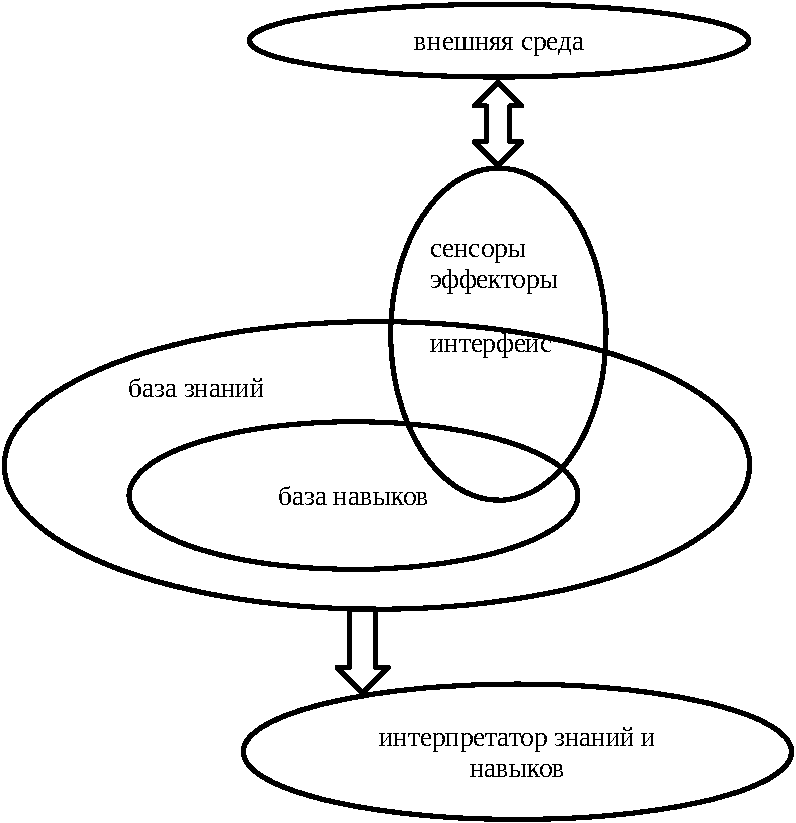
\includegraphics[width=0.5\linewidth]{figures/arch.pdf}\\}

\bigskip
\scnendstruct \scnendcurrentsectioncomment

\end{SCn}

\scsubsection{Предметная область и онтология семантических сетей, семантических языков и семантических моделей баз знаний}
\begin{SCn}

\scnsectionheader{Предметная область и онтология семантических сетей, семантических языков и семантических моделей баз знаний}

\scnstartsubstruct

\scnheader{Предметная область семантических сетей, семантических языков и семантических моделей баз знаний}
\scnsdmainclasssingle{***}
\scnsdclass{смысловое представление информации}
\scnsdrelation{***}

\scnheader{смысловое представление информации}
\scnexplanation{Объективным ориентиром для \textbf{унификации представления информации} в памяти компьютерных систем и ключом к решению многих проблем эволюции компьютерных систем и технологий является \textbf{формализация смысла представляемой информации}.

Согласно В. В. Мартынову~\cite{Martynov}, <<фактически всякая мыслительная деятельность человека (не только научная), как полагают многие ученые, использует внутренний семантический код, на который переводят с естественного языка и с которого переводят на естественный язык. Поразительная способность человека к идентификации огромного множества структурно различных фраз с одинаковым смыслом и способность \textbf{запомнить смысл вне этих фраз} убеждает нас в этом.>>

Приведем также слова И.А. Мельчука~\cite{MelchukST}:

<<Идея была следующая -- язык надо описывать следующим образом: надо уметь записывать смыслы фраз. Не фразы, а их смыслы, что отдельно. Плюс построить систему, которая по смыслу строит фразу. Это та область или тот поворот исследований, при котором интуиция способного лингвиста работает лучше всего: как выразить на данном языке данный смысл. Это -- то, для чего лингвистов учат..

Лингвистический смысл научного текста -- это совсем не то, что ты, читая его, из него извлекаешь. Это, очень грубо говоря, инвариант синонимических парафраз. Ты можешь один и тот же смысл выразить очень многими. Когда ты говоришь, то можешь сказать по-разному: ``Сейчас я налью тебе вина'', или: ``Дай, я тебе предложу вина'', или: ``Не выпить ли нам по бокалу?'', -- все это имеет один и тот же смысл. И вот можно придумать, как записывать этот смысл. Именно его. Не фразу, а смысл. И работать надо от этого смысла к реальным фразам. Синтаксис там по дороге тоже нужен, но он нужен именно по дороге, он не может быть ни конечной целью, ни начальной точкой. Это -- промежуточное дело.>>~\cite{Melchuk}.

Уточнение принципов \textbf{смыслового представления информации} основано, во-первых, на четком противопоставление \textbf{внутреннего языка компьютерной системы}, используемого для хранения информации в памяти компьютера, и \textbf{внешних языков компьютерной системы}, используемых для общения (обмена сообщениями) компьютерной системы с пользователями и другими компьютерными системами (смысловое представление используется исключительно для \textbf{внутреннего представления} информации в памяти компьютерной системы), и, во-вторых, на максимально возможном упрощении синтаксиса внутреннего языка компьютерной системы при обеспечении универсальности  путем исключения из такого внутреннего универсального языка средств, обеспечивающих коммуникационную функцию языка (т. е. обмен сообщениями).

Так, например, для внутреннего языка компьютерной системы излишними являются такие коммуникационные средства языка, как союзы, предлоги, разделители, ограничители, склонения, спряжения и другие.

Внешние языки компьютерной системы могут быть как близки ее внутреннему языку, так и весьма далеки от него (как, например, естественные языки).

\textbf{Смысл} – это \textbf{абстрактная} знаковая конструкция, принадлежащая внутреннему языку компьютерной системы, являющаяся \textbf{инвариантом} максимального класса семантически эквивалентных знаковых конструкций (текстов), принадлежащих самым разным языкам, и удовлетворяющая следующим требованиям:
\begin{scnitemize}
    \item \textbf{универсальность} - возможность представления любой информации;
    \item \textbf{отсутствие синонимии знаков} (многократного вхождения знаков с одинаковыми денотатами);
    \item \textbf{отсутствие дублирования информации} в виде семантически эквивалентных текстов (не путать с логической эквивалентностью);
    \item \textbf{отсутствие омонимичных знаков} (в том числе местоимений);
    \item \textbf{отсутствие у знаков внутренней структуры} (атомарный характер знаков);
    \item \textbf{отсутствие склонений, спряжений} (как следствие отсутствия у знаков внутренней структуры);
    \item \textbf{отсутствие фрагментов} знаковой конструкции, \textbf{не являющихся знаками} (разделителей, ограничителей, и т.д.);
    \item \textbf{выделение знаков связей}, компонентами которых могут быть любые знаки, с которыми знаки связей связываются синтаксически задаваемыми отношениями инцидентности.
\end{scnitemize}

Следствием указанных принципов смыслового представления информации в памяти компьютерной системы является то, что знаки сущностей, входящие в смысловое представление информации, \textbf{не являются именами} (терминами) и, следовательно, не привязаны ни к какому естественному языку и не зависят от субъективных терминотворческих пристрастий различных авторов. Это значит, что при коллективной разработке смыслового представления каких-либо информационных ресурсов терминологические споры исключены.

Следствием указанных принципов смыслового представления информации  является также то, что эти принципы приводят к нелинейным знаковым конструкциям (к графовым структурам), что усложняет реализацию памяти компьютерных систем, но существенно упрощает ее логическую организацию (в частности, ассоциативный доступ).

Нелинейность смыслового представления информации обусловлена тем, что: 
\begin{scnitemize}
    \item каждая описываемая сущность, т.е. сущность, имеющая соответствующий ей знак, может иметь неограниченное число связей с другими описываемыми сущностями;
    \item каждая описываемая сущность в смысловом представлении имеет единственный знак, т.к. синонимия знаков здесь запрещена;
    \item все связи между описываемыми сущностями описываются (отражаются, моделируются) связями между знаками этих описываемых сущностей.
\end{scnitemize}

Суть \textbf{универсального смыслового представления информации} можно сформулировать в виде следующих положений:
\begin{scnitemize}
    \item Смысловая знаковая конструкция трактуется как множество знаков, взаимно-однозначно обозначающих различные сущности (денотаты этих знаков) и множество связей между этими знаками;
    \item Каждая связь между знаками трактуется, с одной стороны, как множество знаков, связываемых этой связью, а, с другой стороны, как описание (отражение, модель) соответствующей связи, которая связывает денотаты указанных знаков или денотаты одних знаков непосредственно с другими знаками, или сами эти знаки. Примером первого вида связи между знаками является связь между знаками материальных сущностей, одна из которых является частью другой. Примером второго вида связи между знаками является связь между знаком множества знаков и одним из знаком, принадлежащих этому множеству, а также связь между знаком и знаком файла, являющегося электронным отражением структуры представления указанного знака во внешних знаковых конструкциях. Примерами третьего вида связи между знаками является связь между синонимичными знаками;
    \item Денотатами знаков могут быть (1) не только конкретные (константные, фиксированные), но и произвольные (переменные, нефиксированные) сущности, "пробегающие"\ различные множества знаков (возможных значений), 
    (2) не только реальные (материальные), но и абстрактные сущности (например, числа, точки различных абстрактных пространств), 
    (3) не только "внешние"\,, но и "внутренние"\ сущности, являющиеся множествами знаков, входящих в состав той же самой знаковой конструкции.
\end{scnitemize}

Ключевым свойством языка смыслового представления информации является однозначность представления информации в памяти каждой компьютерной системы, т. е. отсутствие семантически эквивалентных знаковых конструкций, принадлежащих смысловому языку и хранимых в одной смысловой памяти. При этом логическая эквивалентность таких знаковых конструкций допускается и используются, например, для компактного представления некоторых знаний, хранимых в смысловой памяти.

Тем не менее, логической эквивалентностью хранимых в памяти знаковых конструкций увлекаться не следует, т.к. \textbf{логически эквивалентные} знаковые конструкции -- это представление одного и того же знания, но с помощью \textbf{разных наборов понятий}. В отличие от этого \textbf{семантически эквивалентные} знаковые конструкции -- это представление одного и того же знания с помощью одних и тех же понятий. Очевидно, что многообразие возможных вариантов представления одних и тех же знаний в памяти компьютерной системы существенно усложняет решение задач. Поэтому, полностью исключив \textbf{семантическую эквивалентность} в смысловой памяти, необходимо стремиться к минимизации \textbf{логической эквивалентности}. Для этого необходимо грамотное построение системы используемых понятий в виде иерархической системы формальных онтологий ~\cite{Davydenko2018}.

Важным этапом создания универсального формального способа смыслового кодирования знаний был разработанный В.В. Мартыновым Универсальный Семантический Код (УСК)~\cite{Martynov}.

В качестве \textbf{стандарта} универсального смыслового представления информации \textbf{в памяти компьютерных систем} нами предложен \textbf{\textit{SC-код}} (Semantic Computer Code). В отличие от УСК В.В. Мартынова он, во-первых, носит нелинейный характер и, во-вторых, специально ориентирован на кодирование информации в памяти компьютеров нового поколения, ориентированных на разработку семантически совместимых интеллектуальных систем и названных нами \textbf{семантическими ассоциативными компьютерами}. Более подробно это понятие (\textbf{\textit{SC-код}}) рассмотрено в разделе \textit{Предметная область и онтология внутреннего языка ostis-систем -- SC-кода}. Таким образом, основным лейтмотивом предлагаемого нами смыслового представления информации является ориентация на формальную модель памяти нефоннеймановского компьютера, предназначенного для реализации интеллектуальных систем, использующих смысловое представление информации. Особенностями такого представления являются следующие:
\begin{scnitemize}
    \item ассоциативность;
    \item вся информация заключена в конфигурации связей, т.е. переработка информации сводится к реконфигурации связей (к графодинамическим процессам);
    \item прозрачная семантическая интерпретируемость и, как следствие, семантическая совместимость.
\end{scnitemize}

Неявная привязка к фоннеймановским компьютерам присутствует во всех известных моделях представления знаний. Одним из примеров такой зависимости, является, например, обязательность именования описываемых объектов.}

\scnheader{смысловое представление информации}
\scnadvantages{Почему целесообразен переход к \textit{смысловому представлению информации} в памяти \textit{компьютерной системы}: 
\begin{scnitemize}
    \item \textit{смысловое представление информации} есть \uline{объективный}, не зависящий от субъективизма и многообразия синтаксических решений, способ представления информации;
    \item в рамках смыслового представления существенно упрощается процедура интеграции знаний и погружения новых знаний в \textit{базу знаний};
    \item cущественно упрощается процедура приведения различного вида знаний к общему виду (к согласованной системе используемых понятий);
    \item cущественно упрощается процедура интеграции различных \textit{~решателей задач~} и целых \textit{компьютерных систем}; 
    \item существенно упрощается автоматизация перманентного процесса поддержки семантической совместимости (согласованности понятий и онтологий) для \textit{компьютерных систем} в условиях их постоянного совершенствования;
    \item в рамках смыслового представления информации достаточно легко осуществляется переход от информационных конструкций к информационным метаконструкциям путем введения узлов семантической сети, обозначающих информационные конструкции, а также дуг, связывающих эти узлы со всеми элементами обозначаемой им информационной конструкции;
    \item на основе \textit{стандарта смыслового представления информации} существенно упрощается интеграция различных дисциплин в области искусственного интеллекта, т.е. построение общей формальной теории интеллектуальных компьютерных систем, так как для построения общей формальной модели интеллектуальных компьютерных систем необходим базовый язык, в рамках которого можно было бы легко переходить от информации (от знаний) к \textbf{метаинформации} (к метазнаниям, к спецификациям исходных знаний).  Это подтверждается тем, что:
    \begin{scnitemizeii}
        \item подавляющее число понятий искусственного интеллекта носит метаязыковой характер;
        \item формальное смысловое уточнение почти каждого понятия искусственного интеллекта требует предшествующего формального уточнения соответствующего языка-объекта. Так, например, как можно строго говорить о языке онтологий (т.е. языке спецификации предметных областей), не уточнив язык представления самих этих предметных областей. Как можно строго говорить о языке описания способов обработки информации, не уточнив язык представления самой этой обрабатываемой информации.
    \end{scnitemizeii}
\end{scnitemize}}

\scnendstruct

\end{SCn}

\scsubsection{Предметная область и онтология агентно-ориентированных семантических моделей решателей задач}
\begin{SCn}

\scnsectionheader{\currentname}

\scnstartsubstruct

\scnheader{Предметная область многоагентных моделей решения задач, основанных на смысловом представлении информации}
\scniselement{предметная область}
\scnsdmainclasssingle{многоагентный подход к обработке информации}
\scnsdclass{интеграция решателей задач}
\scnsdrelation{совместимость моделей решения задач*}

\scnheader{многоагентный подход к обработке информации}
\scnnote{В качестве основы унификации принципов обработки информации в компьютерных системах предлагается использовать \textbf{многоагентный подход}, обладающий рядом важных достоинств.}
\scnrelfromset{достоинства}{\scnfileitem{Автономность (независимость) агентов, что позволяет локализовать изменения, вносимые в систему при ее эволюции, и снизить соответствующие трудозатраты.};
\scnfileitem{Децентрализация обработки, т.е. отсутствие единого контролирующего центра, что также позволяет локализовать вносимые в систему изменения.};
\scnfileitem{Возможность параллельной работы разных информационных процессов, соответствующих как одному агенту, так и разным агентам, как следствие, -- возможность распределенного решения задач. Однако возможность параллельного выполнения информационных процессов подразумевает наличие средств синхронизации такого выполнения, разработка которых является отдельной задачей.};
\scnfileitem{Активность агентов и многоагентной системы в целом, дающая возможность при общении с такой системой не указывать явно способ решения поставленной задачи, а формулировать задачу в \uline{декларативном ключе}.}}
\scnaddlevel{1}
	\scnrelfrom{источник}{\scncite{Wooldridge2009}}
\scnaddlevel{-1}
\scnrelfromset{недостатки современного состояния}{\scnfileitem{Знания агента представляются при помощи узкоспециализированных языков, зачастую не предназначенных для представления знаний в широком смысле и онтологий в частности.};
\scnfileitem{Большинство современных многоагентных систем предполагает, что взаимодействие агентов осуществляется путем обмена сообщениями непосредственно от агента к агенту.};
\scnfileitem{Логический уровень взаимодействия агентов жестко привязан к физическому уровню реализации многоагентной системы.};
\scnfileitem{Среда, с которой взаимодействуют агенты, уточняется отдельно разработчиком для каждой многоагентной системы, что приводит к существенным накладным расходам и несовместимости таких многоагентных систем.}}
\scnaddlevel{1}
\scnrelfromset{принципы устранения}{
\scnfileitem{Коммуникацию агентов предлагается осуществлять путем спецификации (в общей памяти компьютерной системы) действий (процессов), выполняемых агентами и направленных на решение задач.}
\scnaddlevel{1}
	\scntext{детализация}{Коммуникацию агентов предлагается осуществлять по принципу ``доски объявлений'', однако в отличие от классического подхода в роли сообщений выступают спецификации в общей семантической памяти выполняемых агентами действий (процессов), направленных на решение каких-либо задач, а в роли среды коммуникации выступает сама эта семантическая память. Такой подход позволяет: 
	\begin{scnitemize}
		\item исключить необходимость разработки специализированного языка для обмена сообщениями;
		\item обеспечить "обезличенность"{} общения, т. е. каждый из агентов в общем случае не знает, какие еще агенты есть в системе, кем сформулирован и кому адресован тот или иной запрос. Таким образом, добавление или удаление агентов в систему не приводит к изменениям в других агентах, что обеспечивает модифицируемость всей системы;
		\item агентам, в том числе конечному пользователю, формулировать задачи в \uline{декларативном ключе}, т. е. не указывать для каждой задачи способ ее решения. Таким образом, агенту заранее не нужно знать, каким образом система решит ту или иную задачу, достаточно лишь специфицировать конечный результат;
		\item сделать средства коммуникации агентов и синхронизации их деятельности более понятными разработчику и пользователю системы, не требующими изучения специальных низкоуровневых типов данных и форматов сообщений. Таким образом повышается доступность предлагаемых решений широкому кругу разработчиков.
	\end{scnitemize}
	Следует отметить, что такой подход позволяет при необходимости организовать обмен сообщениями между агентами напрямую и, таким образом, может являться основой для моделирования многоагентных систем, предполагающих другие способы взаимодействия между агентами.}
\scnaddlevel{-1}
;
\scnfileitem{В роли внешней среды для агентов выступает та же общая память, в которой формулируются задачи и посредством которой осуществляется взаимодействие агентов. Такой подход обеспечивает унификацию среды для различных систем агентов, что, в свою очередь, обеспечивает их совместимость.};
\scnfileitem{Спецификация каждого агента описывается средствами языка представления знаний в той же памяти, что позволяет:
	\begin{scnitemize}
		\item минимизировать число специализированных средств, необходимых для спецификации агентов, как языковых, так и инструментальных;
		\item с одной стороны -- минимизировать необходимую в общем случае спецификацию агента, которая включает условие его инициирования и программу, описывающую алгоритм работы агента, с другой стороны -- обеспечить возможность произвольного расширения спецификации для каждого конкретного случая, в том числе возможность реализации различных современных моделей спецификации агента.
	\end{scnitemize}};
\scnfileitem{Синхронизацию деятельности агентов предполагается осуществлять на уровне выполняемых ими процессов, направленных на решение тех или иных задач в общей семантической памяти. Таким образом, каждый агент трактуется как некий абстрактный процессор, способный решать задачи определенного класса. При таком подходе необходимо решить задачу обеспечения взаимодействия параллельных асинхронных процессов в общей семантической памяти, для решения которой можно заимствовать и адаптировать решения, применяемые в традиционной линейной памяти. При этом вводится дополнительный класс агентов -- метаагенты, задачей которых является решение возникающих проблемных ситуаций, таких как взаимоблокировки};
\scnfileitem{Каждый информационный процесс в любой момент времени имеет ассоциативный доступ к необходимым фрагментам базы знаний, хранящейся в семантической памяти, за исключением фрагментов, заблокированных другими процессами в соответствии с соответствующим механизмом синхронизации. Таким образом, с одной стороны, исключается необходимость хранения каждым агентом информации о внешней среде, с другой стороны, каждый агент, как и в классических многоагентных системах, обладает только частью всей информации, необходимой для решения задачи.\\
Важно отметить, что в общем случае невозможно априори предсказать, какие именно знания, модели и способы решения задач понадобятся системе для решения конкретной задачи. В связи с этим необходимо обеспечить, с одной стороны, возможность доступа ко всем необходимым фрагментам базы знаний (в пределе -- ко всей базе знаний), с другой стороны -- иметь возможность локализовать область поиска пути решения задачи, например, рамками одной \textit{предметной области}.\\
Каждый из агентов обладает набором ключевых элементов (как правило, понятий), которые он использует в качестве отправных точек при ассоциативном поиске в рамках базы знаний. Набор таких элементов для каждого агента уточняется на этапах проектирования многоагентной системы в соответствии с рассматриваемой ниже методикой. Уменьшение числа ключевых элементов агента делает его более универсальным, однако снижает эффективность его работы за счет необходимости выполнения дополнительных  операций.}}
\scnaddlevel{1}
\scnnote{Предлагаемый подход позволяет рассматривать решатель задач как иерархическую систему. Некий целостный коллектив агентов, реализующий какую-либо подсистему решателя (например, машину дедуктивного вывода, подсистему верификации базы знаний и т. д.), может рассматриваться как единый неатомарный агент, поскольку коллективы агентов и отдельные агенты работают в соответствии с одними и теми же принципами.}
\scnaddlevel{-2}

\scnheader{совместимость моделей решения задач*}
\scnnote{\textbf{\textit{совместимость моделей решения задач*}} -- это возможность одновременного использования разными моделями решения задач одних и тех же информационных ресурсов.}
\scnrelfromset{принципы реализации}{
\scnfileitem{Вся информация, хранимая в памяти каждой ostis-системы и используемая \textit{\textbf{решателем задач}} (как собственно обрабатываемая информация, так и хранимые в памяти интерпретируемые методы, например, различного вида программы), записывается в форме смыслового представления этой информации}; 
\scnfileitem{Собственно решение каждой задачи осуществляется коллективом агентов, работающих над общей для них смысловой (семантической) памятью и выполняющих интерпретацию хранимых в этой же памяти \textit{методов}.}}

\scnheader{интеграция решателей задач}
\scnsubset{процесс}
\scnrelfromvector{алгоритм реализации}{
\scnfileitem{Объединение множества методов первого решателя и множества методов второго решателя};	
\scnfileitem{Интеграция множества методов первого решателя и множества методов второго решателя путем взаимного погружения соответствующих информационных конструкций друг в друга, т.е. путем склеивания синонимов, а также путем выравнивания используемых ими понятий.};
\scnfileitem{Объединение множества агентов, входящих в состав первого решателя, со множеством агентов, входящих во второй решатель задач.}}
\scnexplanation{Таким образом, унификация моделей решения задач путем приведения этих моделей к виду семантических моделей (т. е. моделей обработки информации, представленной в смысловой форме) повышает уровень совместимости этих моделей благодаря наличию прозрачной процедуры интеграции информации, представленной в смысловой форме, и тривиальной процедуры объединения множеств \textit{агентов}. Простота процедуры объединения множеств \textit{агентов}, соответствующих разным решателя задач, обусловлена тем, что непосредственного взаимодействия между этими агентами нет, а инициирование каждого из них определяется им самим, а также \uline{текущим состоянием} хранимой в памяти информации.}

\bigskip

\scnendstruct \scnendcurrentsectioncomment

\end{SCn}

\scsubsection{Предметная область и онтология семантических моделей интерфейсов компьютерных систем}

\scsectionfinish{sem_mod_comp_sys}

\begin{SCn}

\scnsectionheader{Предметная область и онтология семантических моделей компьютерных систем}

\scnstartsubstruct

\scnheader{семантическая совместимость компьютерных систем}
\scnexplanation{Уровень совместимости \textit{компьютерных систем} определяется трудоемкостью реализации процедур интеграции (объединения, соединения знаний этих систем), а также трудоемкостью и глубиной интеграции входящих в эти системы \textit{решателей задач} (навыков и интерпретаторов этих навыков). Подчеркнем при этом, что интеграция интеграции рознь -- от эклектики до гибридности и синергетичности дистанция огромного размера.

Совместимые \textit{компьютерные системы} -- это компьютерные системы, для которых существует автоматически выполняемая процедура их интеграции, превращающая эти системы в единую \textbf{\textit{гибридную систему}}, в рамках которой каждая исходная компьютерная система в процессе своего функционирования может свободно использовать любые необходимые информационные ресурсы (знания и навыки), входящие в состав другой исходной компьютерной системы.

Целостную \textit{компьютерную систему} можно рассматривать как решатель задач, интегрировавший несколько моделей решения задач и обладающий средствами взаимодействия с внешней для себя средой (с другими компьютерными системами, с пользователями).

Таким образом, для того, чтобы повысить уровень совместимости \textit{компьютерных систем}, необходимо преобразовать их к виду \textit{многоагентных систем}, работающих над общей семантической памятью, в которой информация представлена семантическими сетями. Такие \textit{компьютерные системы} не всегда целесообразно непосредственно объединять (интегрировать) в более крупные \textit{компьютерные системы}. Иногда целесообразнее их объединять в \textit{коллективы взаимодействующих компьютерных систем}. Но при создании таких коллективов компьютерных систем унификация и совместимость таких систем также очень важны, т.к. существенно упрощают обеспечение высокого уровня их взаимопонимания. Так, например, противоречия между компьютерными системами, входящими в коллектив, можно обнаруживать путем анализа на непротиворечивость \textbf{\textit{виртуальной объединенной базы знаний}} этого коллектива. Более того, непротиворечивость указанной виртуальной базы знаний можно считать одним из критериев семантической совместимости систем, входящих в соответствующий коллектив.}

\scnheader{семантическая компьютерная система}
\scnexplanation{Предлагаемое нами устранение проблем современных информационных технологий путем перехода к \textit{смысловому представлению информации} в памяти компьютерных систем фактически преобразует современные компьютерные системы (в том числе и современные интеллектуальные системы) в \textit{\textbf{семантические компьютерные системы}}, которые, следовательно, являются не альтернативной ветвью развития \textit{компьютерных систем}, а естественным этапом их эволюции, направленным на обеспечение высокого уровня их обучаемости и, в первую очередь, \textbf{совместимости}.

Архитектура \textit{семантических компьютерных систем} (см. \textit{Рис. Архитектура семантических компьютерных систем}) практически совпадает с архитектурой интеллектуальных компьютерных систем, основанных на знаниях. Отличие здесь заключаются в том, что в \textit{семантических компьютерных системах}:
\begin{scnitemize}
    \item база знаний имеет смысловое представление;
    \item интерпретатор знаний и навыков представляет собой коллектив \textit{агентов}, осуществляющих обработку \textit{базы знаний}.
\end{scnitemize}

Как следствие этого, \textit{семантические компьютерные системы} обладают высоким уровнем обучаемости, т.е. способностью быстро приобретать новые и совершенствовать уже приобретенные знания и навыки и при этом не иметь никаких ограничений на вид приобретаемых и совершенствуемых ею знаний и навыков, а также на их совместное использование.

Более того, при согласовании соответствующих стандартов, а также при перманентном совершенствовании этих стандартов и при грамотной их поддержке в условиях интенсивной эволюции как самих стандартов, так и \textit{семантических компьютерных систем} (речь идет о постоянной поддержке соответствия между текущим состоянием компьютерных систем и текущим состоянием эволюционируемых стандартов), \textit{семантические компьютерные системы} и их компоненты обладают весьма высокой степенью совместимости.

Это, в свою очередь, практически исключает дублирование инженерных решений и дает возможность существенно ускорить разработку \textit{семантических компьютерных систем} с помощью постоянно расширяемой библиотеки многократно используемых и совместимых между собой компонентов. 

Основным лейтмотивом перехода от современных компьютерных систем (в том числе интеллектуальных) к семантическим компьютерным системам, т.е. компьютерным системам, основанным на смысловом представлении всей информации, хранимой в ее памяти, является создание \textit{\textbf{общей семантической теории компьютерных систем}}, включающей в себя:
\begin{scnitemize}
    \item cемантическую теорию знаний и баз знаний;
    \item семантическую теорию задач и моделей их решения;
    \item cемантическую теорию взаимодействия информационных процессов;
    \item cемантическую теорию пользовательских и, в том числе, естественно языковых интерфейсов;
    \item cемантическую теорию невербальных сенсорно-эффекторных интерфейсов;
    \item теорию универсальных интерпретаторов семантических моделей компьютерных систем и, в частности, теорию семантических компьютеров.
\end{scnitemize}

Эпицентром следующего этапа развития информационных технологий является решение проблемы обеспечения \textbf{семантической совместимости} \textit{компьютерных систем} и их компонентов. Для решения этой проблемы необходим
\begin{scnitemize}
    \item переход от традиционных компьютерных систем и от современных интеллектуальных систем к \textit{семантическим компьютерным системам};
    \item разработка \textit{стандарта семантических компьютерных систем}.
\end{scnitemize}    
    
Очевидно, что \textit{семантические компьютерные системы} являются компьютерными системами нового поколения, устраняющие многие недостатки современных компьютерных систем. Но для массовой разработки таких систем необходима соответствующая технология, которая должна включать в себя  

\begin{scnitemize}        
    \item теорию \textit{семантических компьютерных систем} и комплекс всех стандартов, обеспечивающих совместимость разрабатываемых систем;
    \item методы и средства проектирования \textit{семантических компьютерных систем};
    \item методы и средства перманентного совершенствования самой технологии.
\end{scnitemize}
}

\scnheader{Рис. Архитектура семантических компьютерных систем}
\scneqfile{\\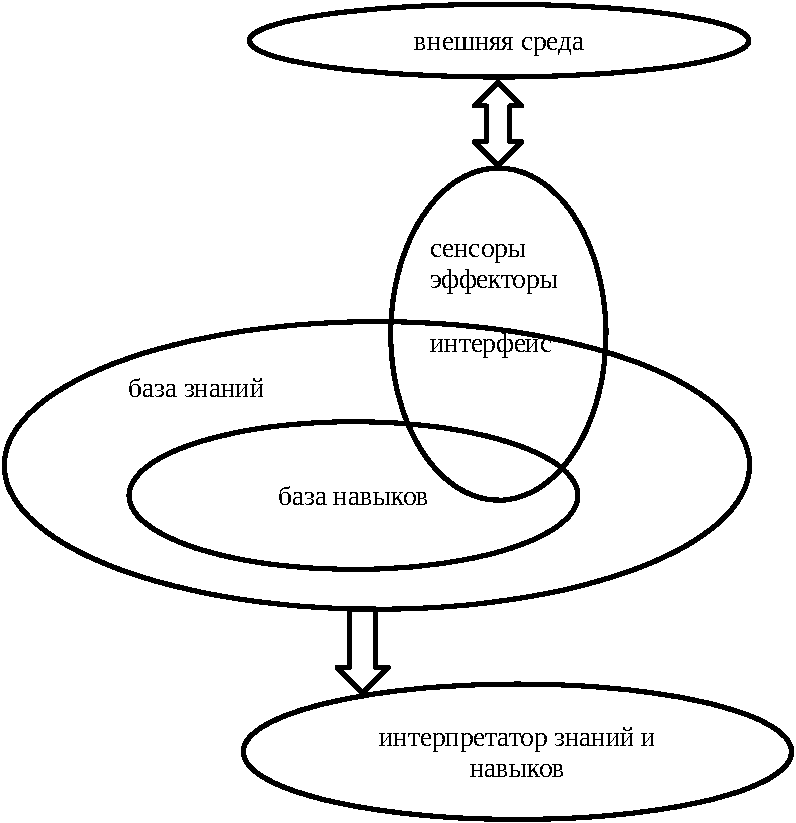
\includegraphics[width=0.5\linewidth]{figures/arch.pdf}\\}

\scnendstruct

\end{SCn}
